\chapter{Stellar Component}
	\label{cha:stellar}


The rest of this chapter is structured as follows: firstly we present the kinematic maps for the stellar component of the galaxy (section \ref{sec:stellarKin}) and a look at how they fit on the $\lambda_{R_e}$--ellipticity plane, then, in section \ref{sec:pop} we investigate the stellar populations using the absorption line strength. We conclude by looking at the odd-one-out of the sample NGC 612 in section \ref{sec:NGC612}

\section{Kinematics}
	\label{sec:stellarKin}

	\subsection{Maps}
		\label{subsec:maps}

		% \begin{figure*}
      \centering
      \includegraphics[width=0.245\textwidth]{Vmaps/ngc0612_stellar_sigma.png}
      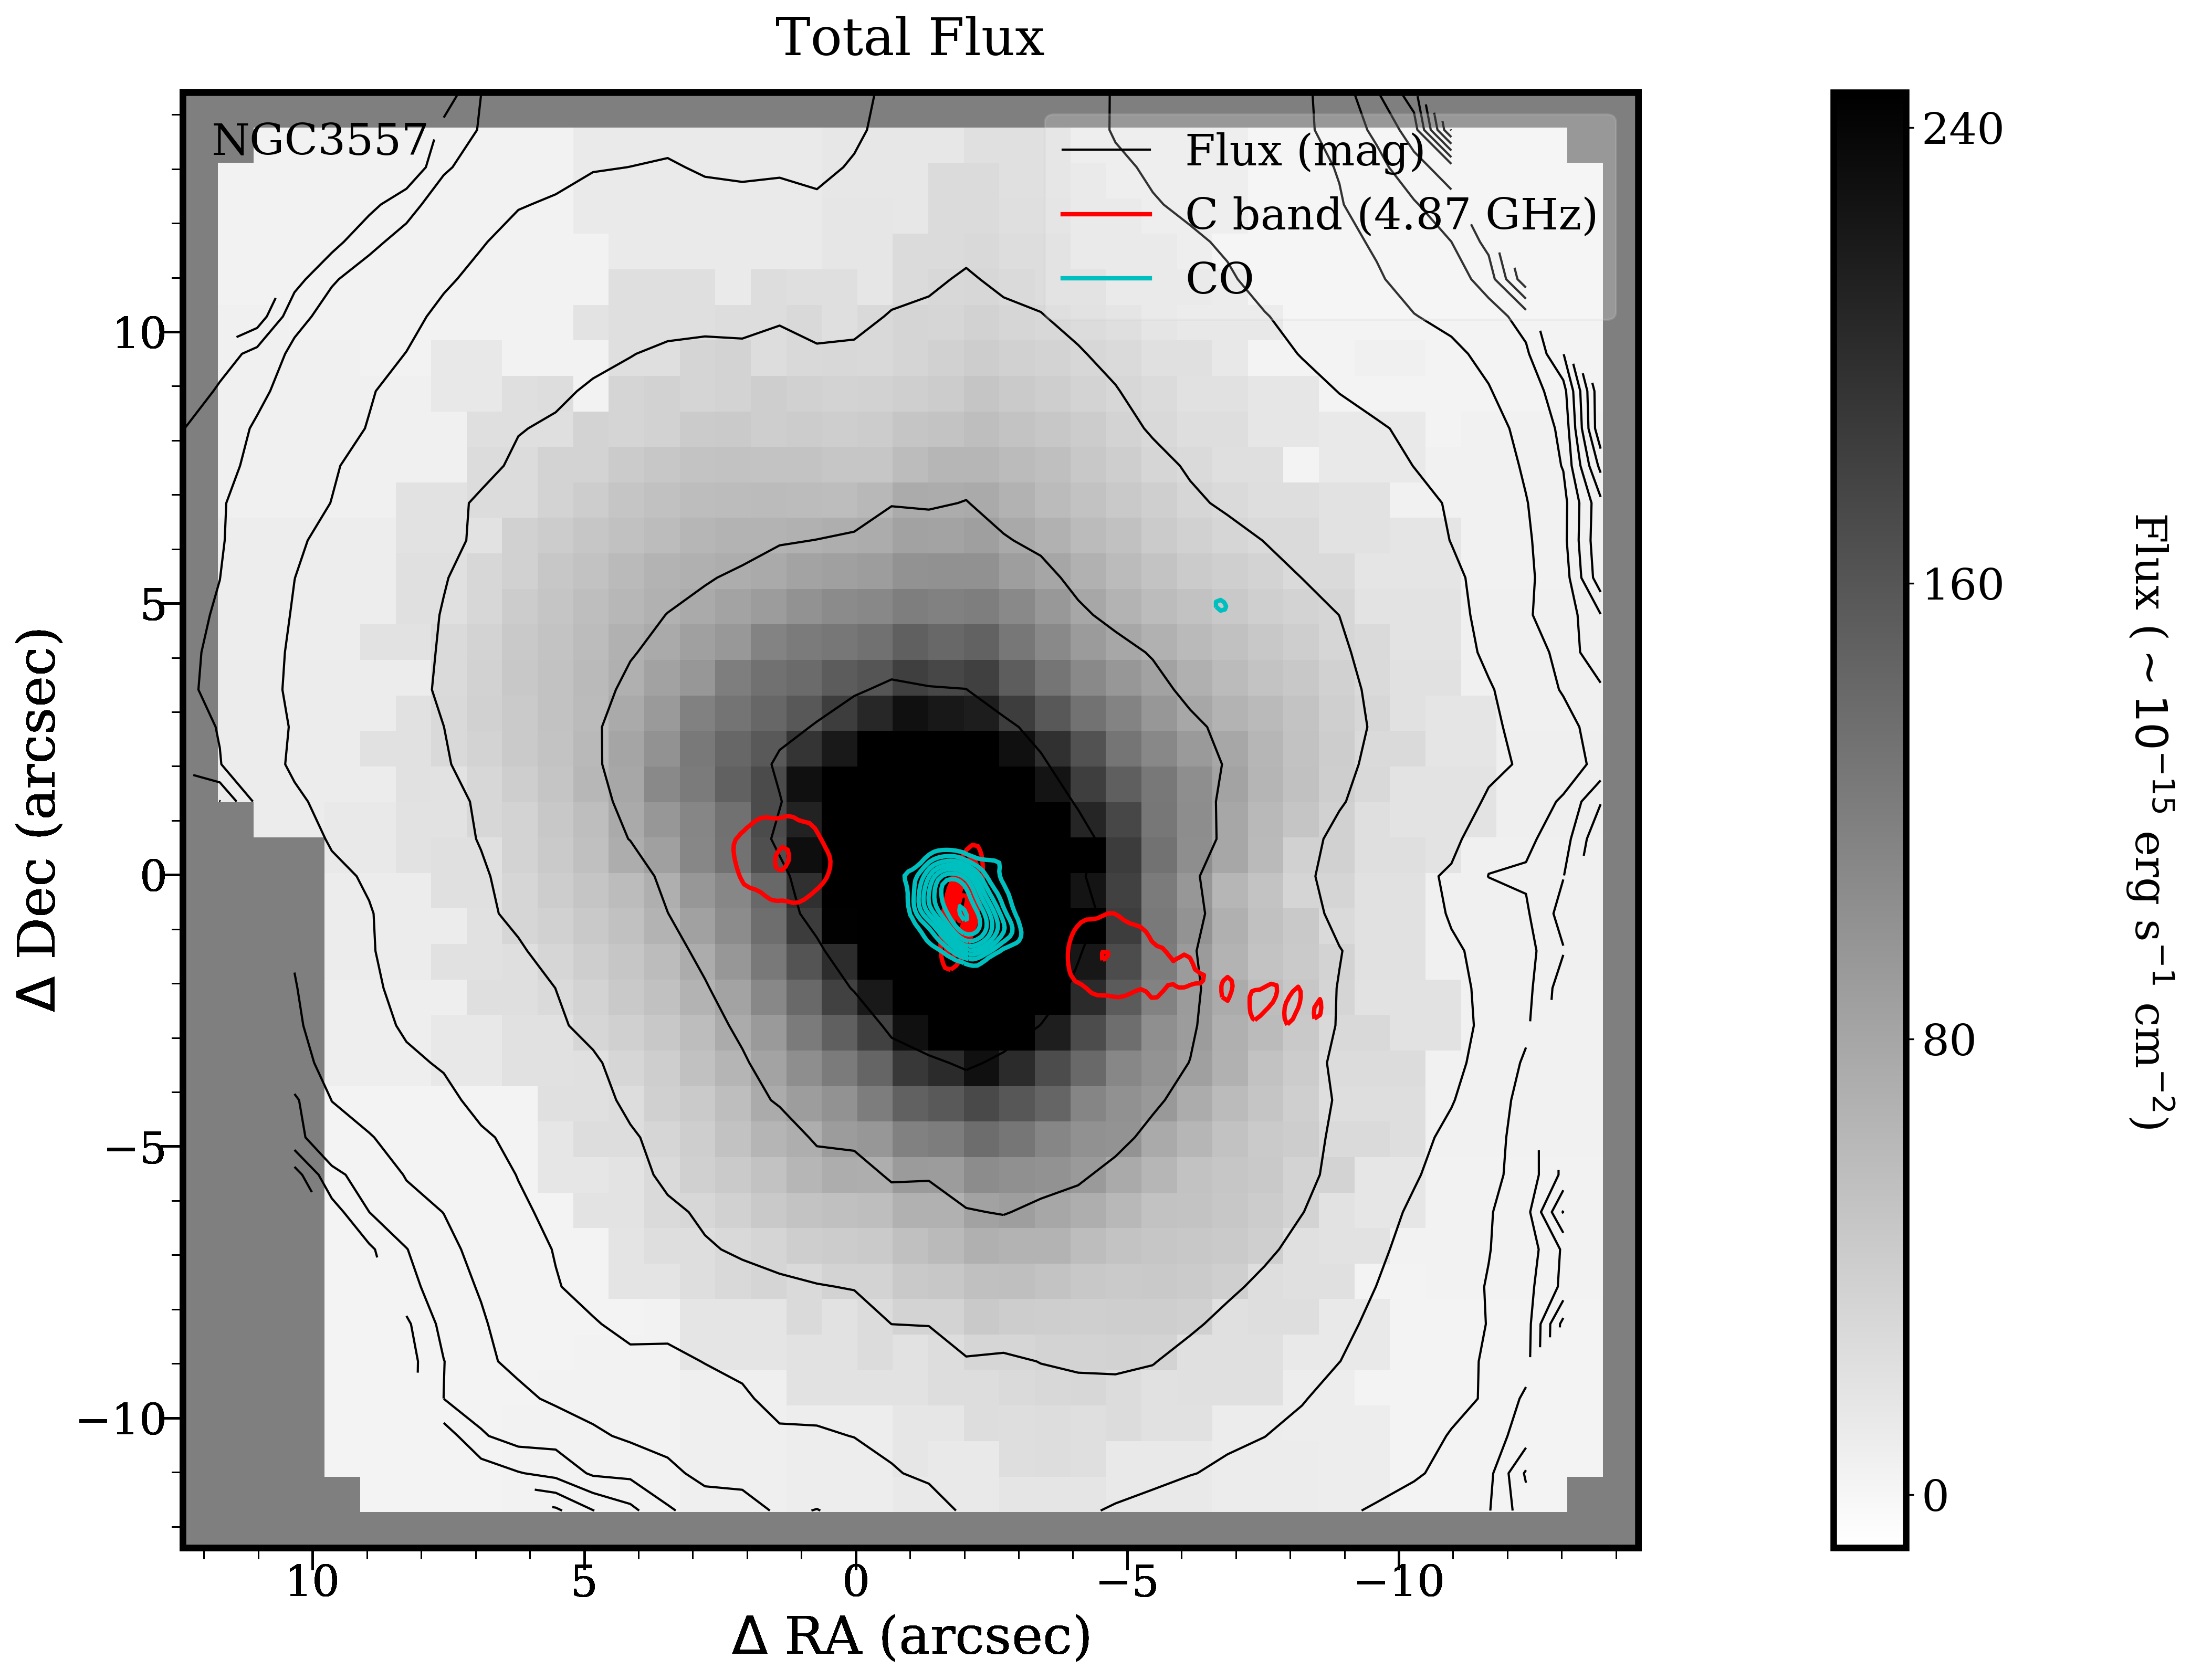
\includegraphics[width=0.245\textwidth]{Vmaps/ngc3557_stellar_img.png}
      \includegraphics[width=0.245\textwidth]{Vmaps/ngc3100_stellar_img.png}
      \includegraphics[width=0.245\textwidth]{Vmaps/ic1459_stellar_img.png}
      \includegraphics[width=0.245\textwidth]{Vmaps/pks0718-34_stellar_img.png}
      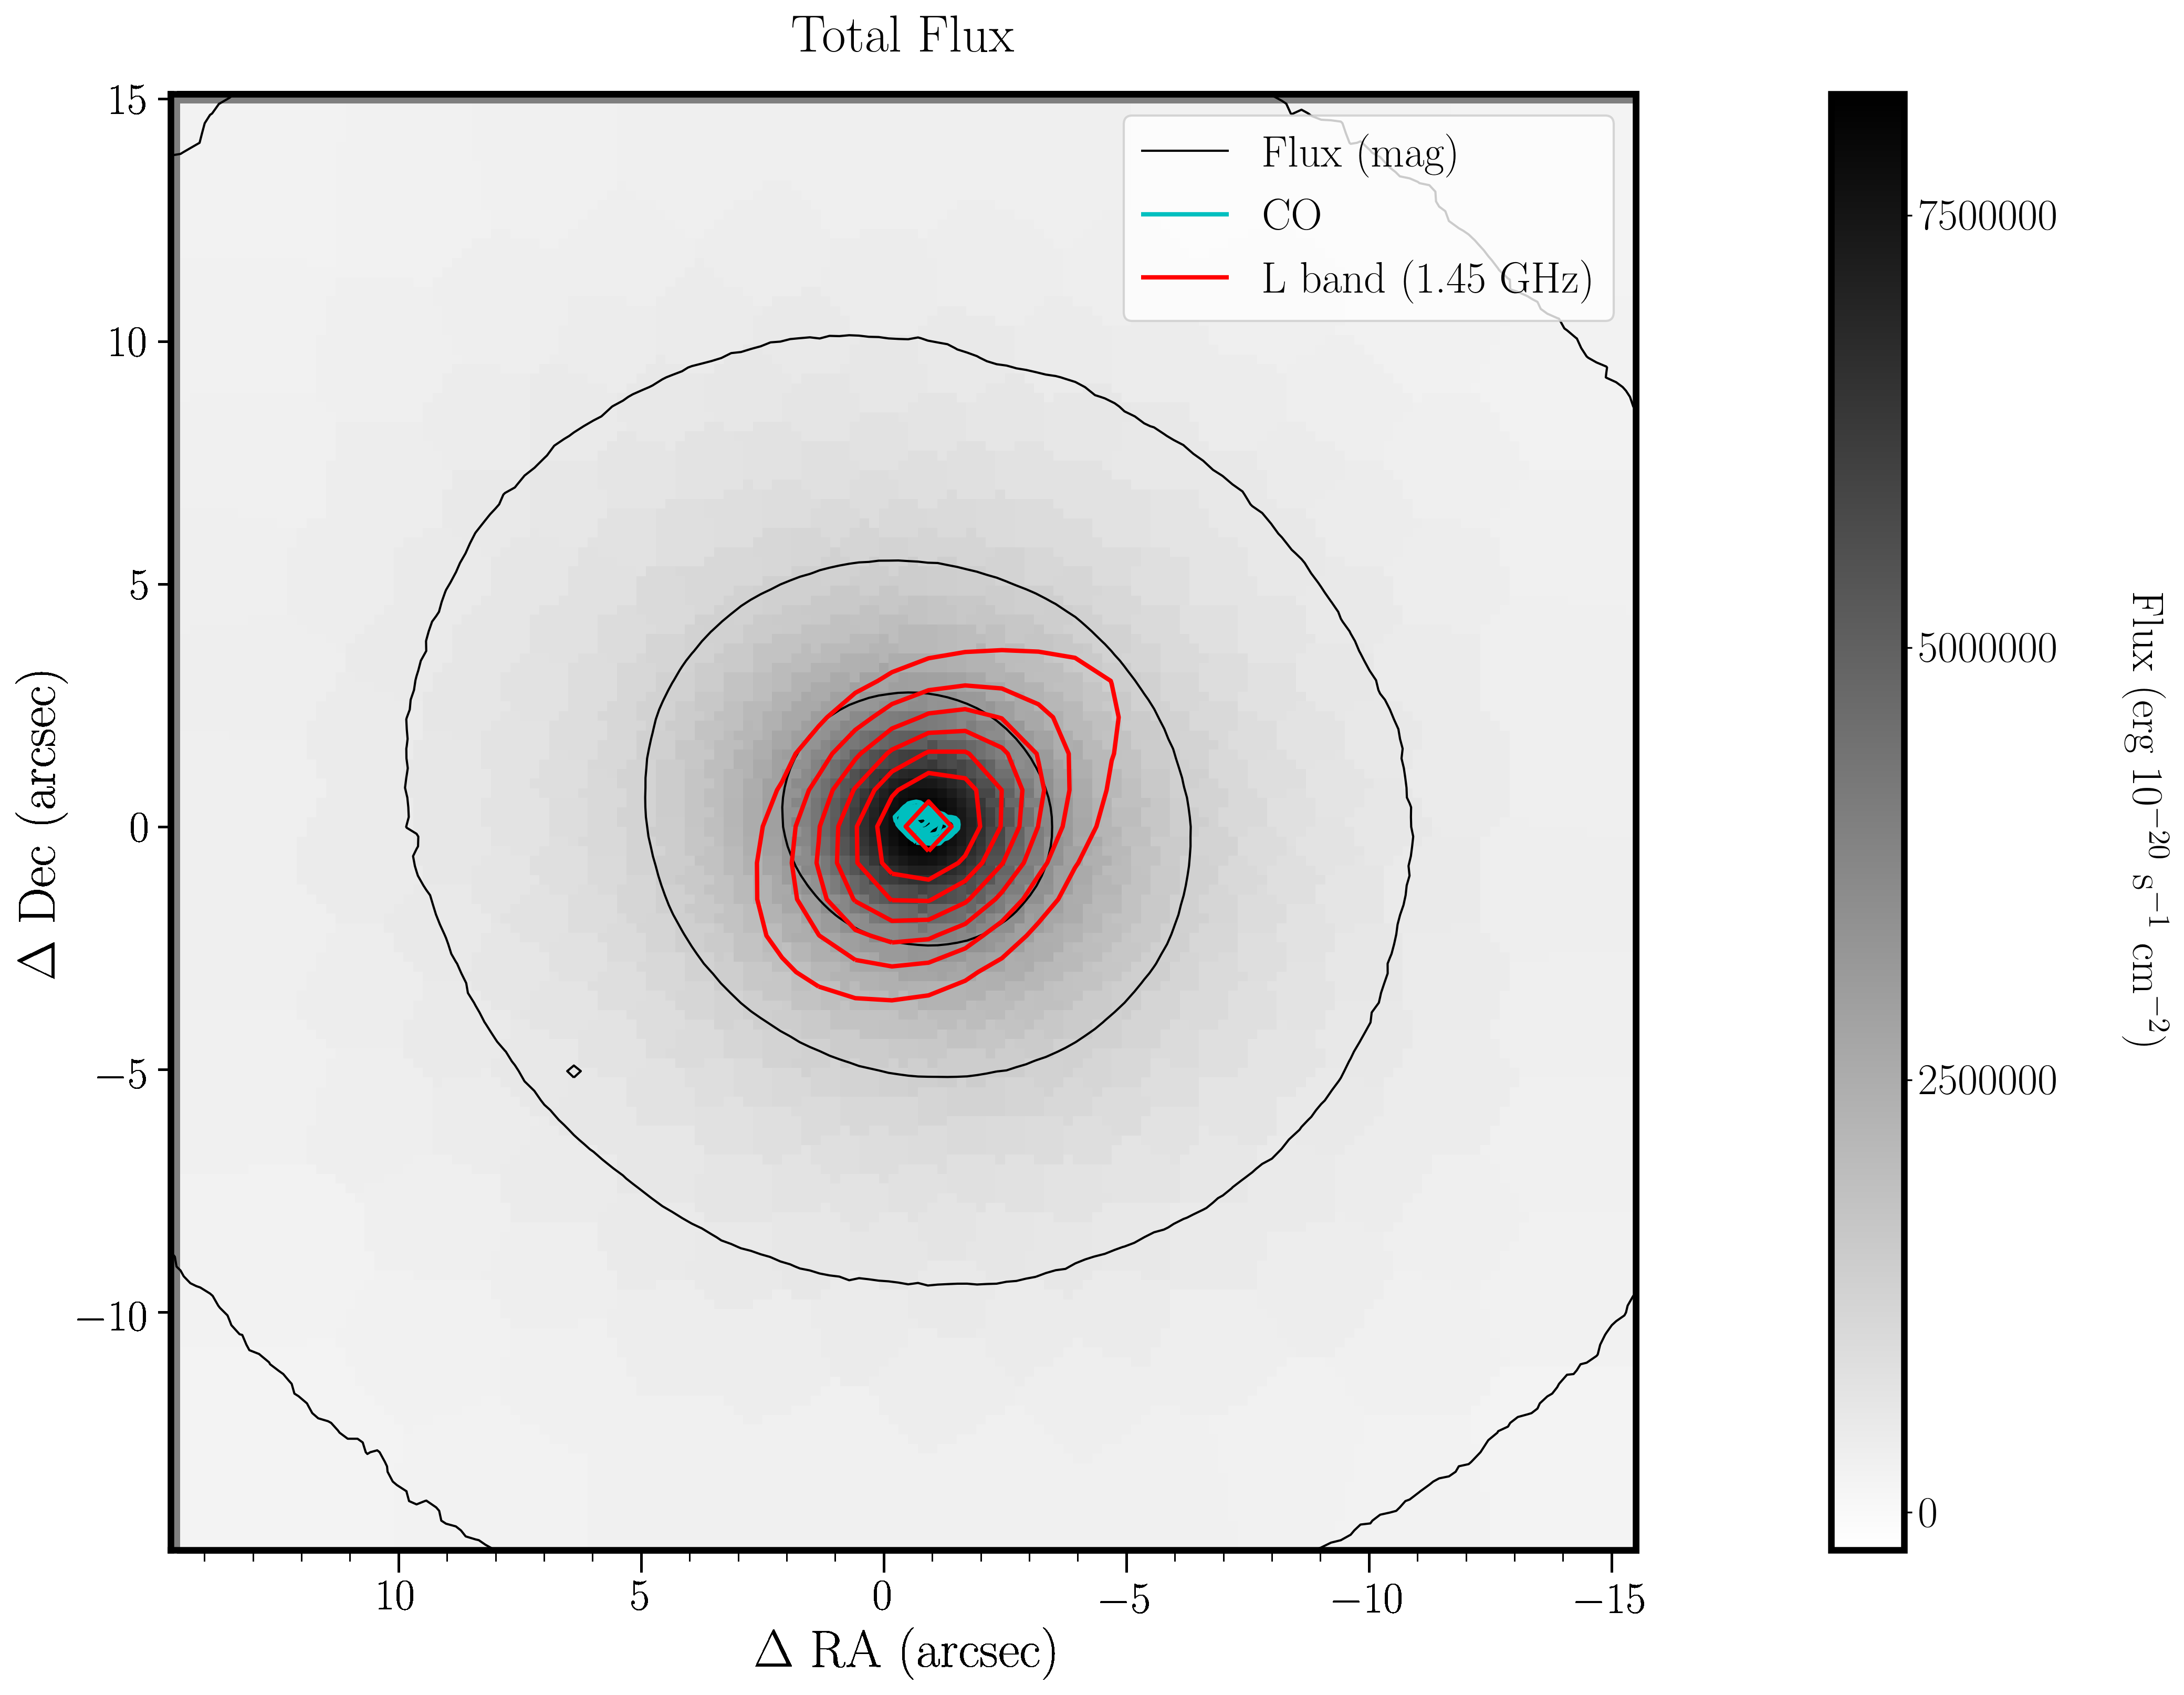
\includegraphics[width=0.245\textwidth]{Vmaps/ic4296_stellar_img.png}
      \includegraphics[width=0.245\textwidth]{Vmaps/ngc7075_stellar_img.png}
      \includegraphics[width=0.245\textwidth]{Vmaps/ic1531_stellar_img.png}
      \includegraphics[width=0.245\textwidth]{Vmaps/ngc1399_stellar_img.png}
      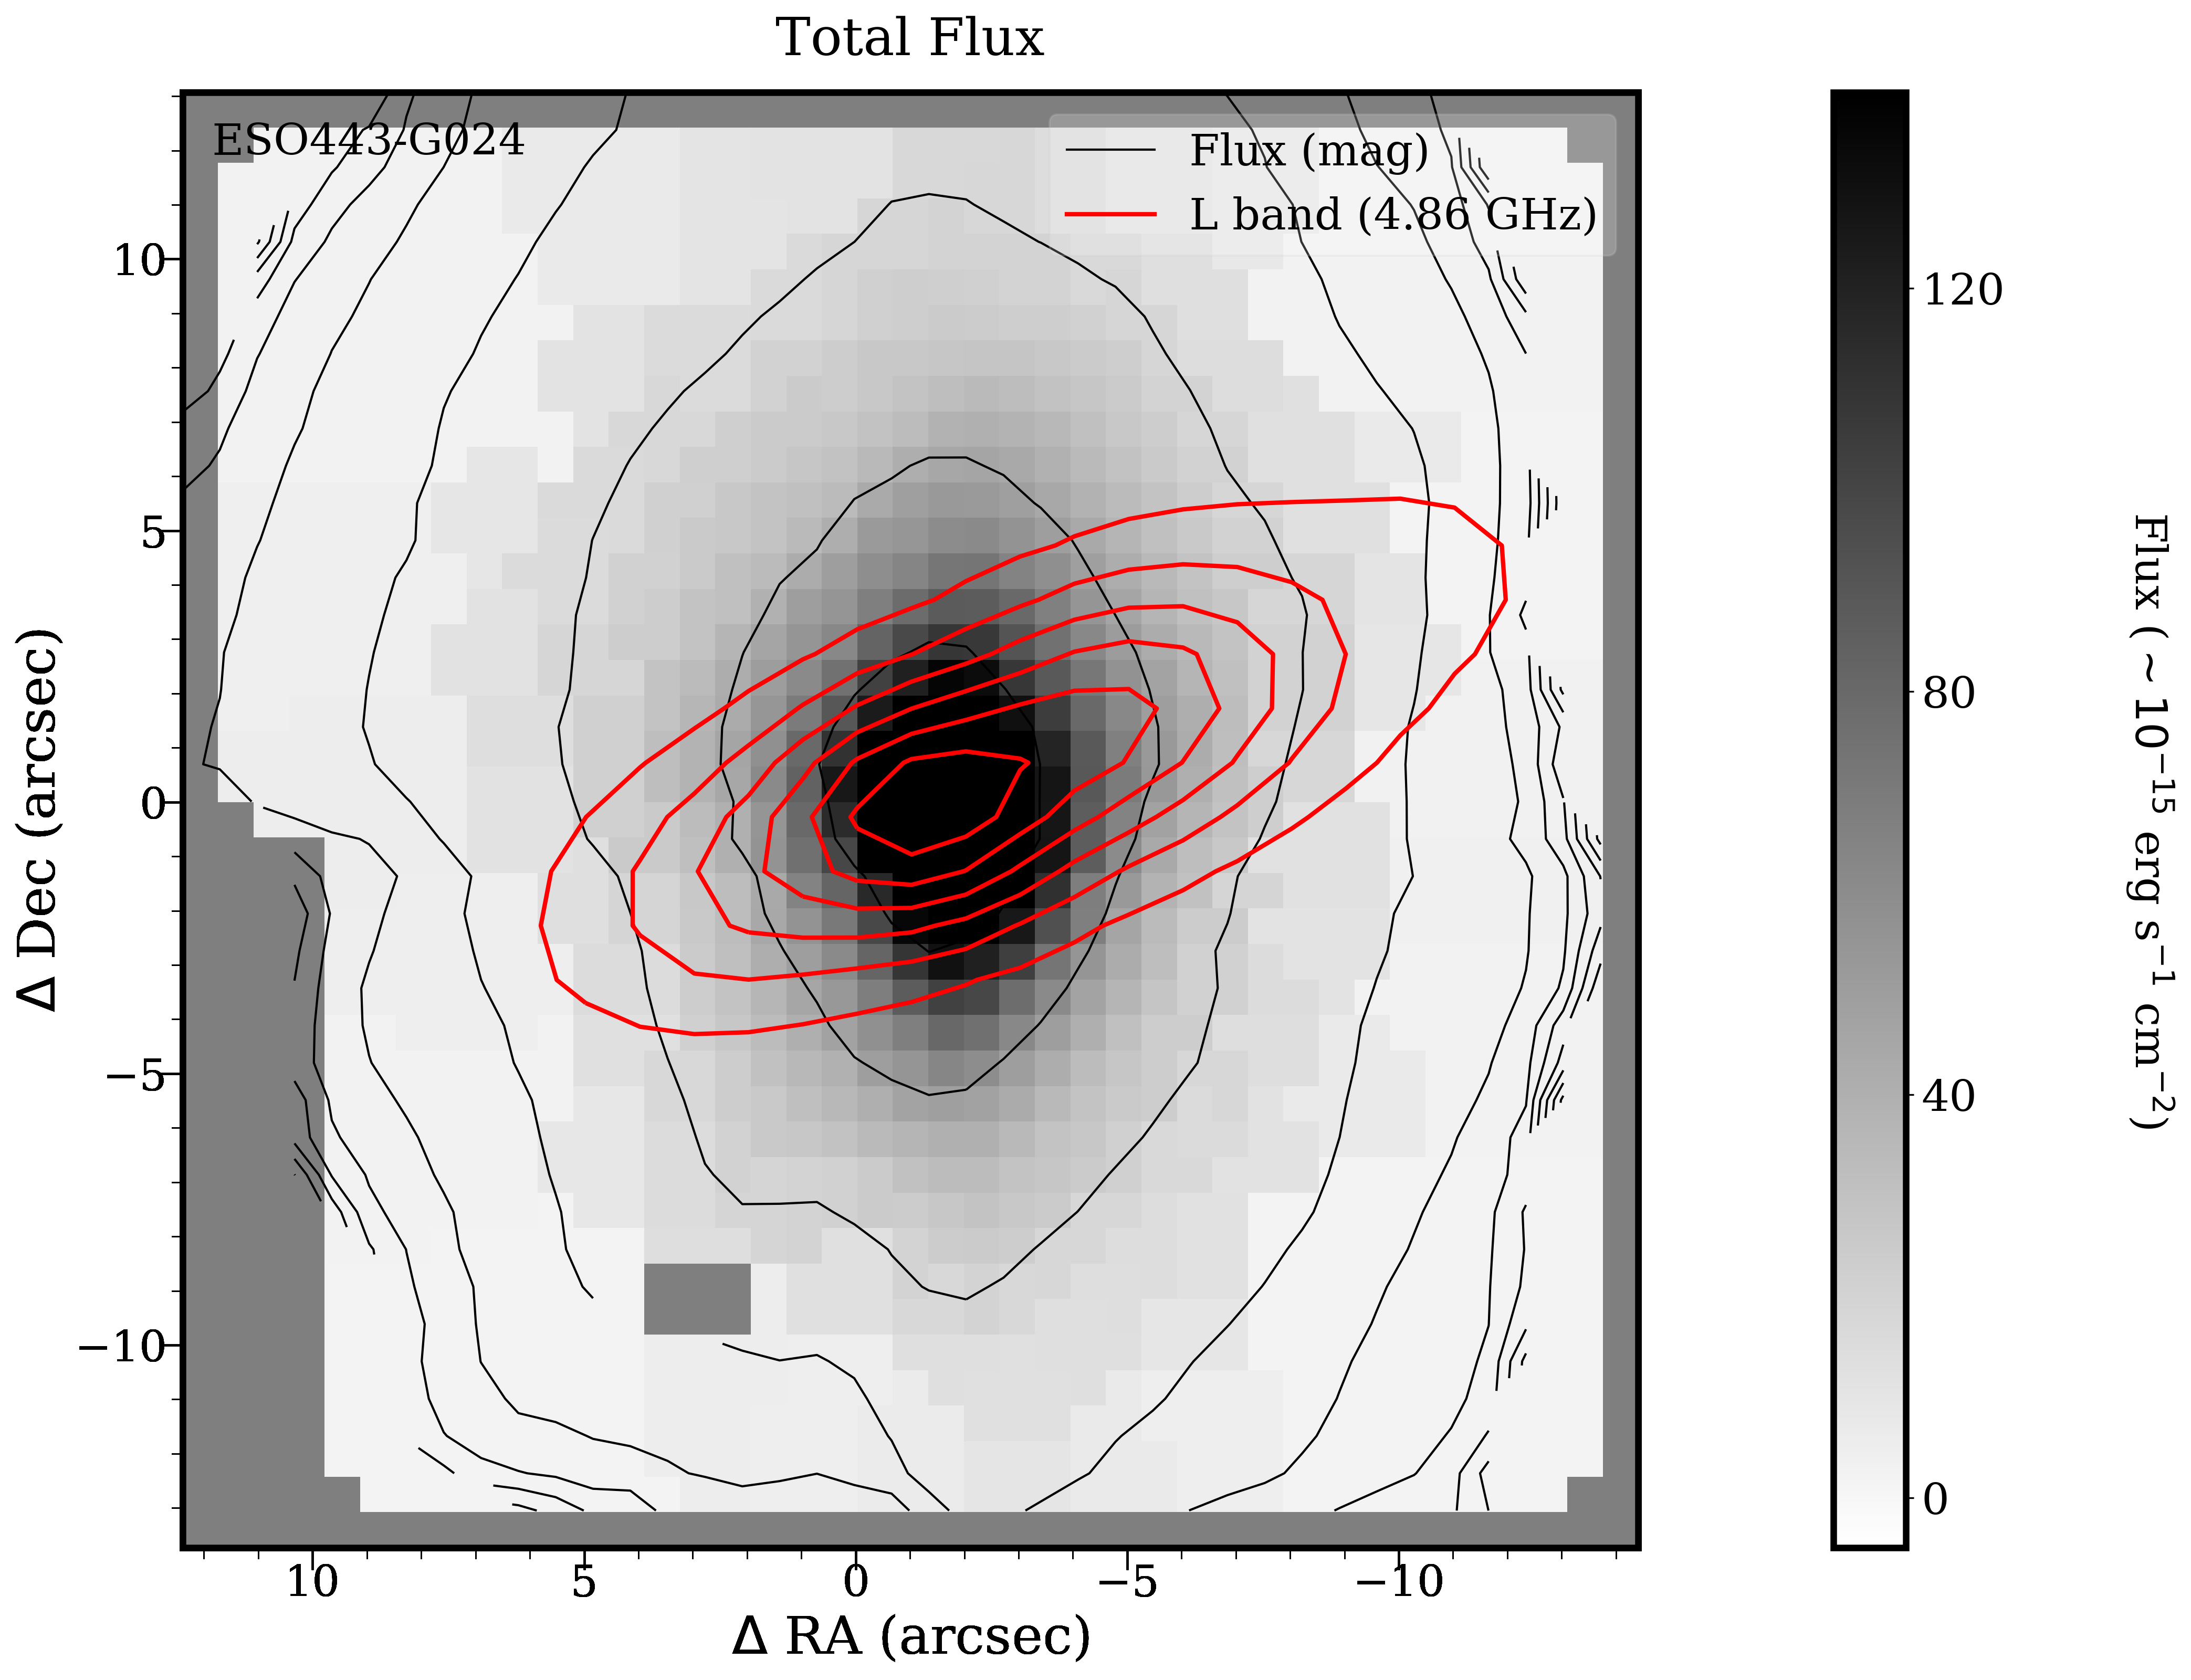
\includegraphics[width=0.245\textwidth]{Vmaps/eso443-g024_stellar_img.png}
      \caption[VIMOS images]{Image for each galaxy in the VIMOS sample. Plots are ordered roughly in peak stellar velocity, with flux contours in black, CO from ALMA in cyan and radio from VLA in red. The radio band displaied is shown in the legend of each plot and depends on what data is avaliable in the archive and which images had a similar resolution and and scale}
      \label{fig:Vstellar_img}
\end{figure*}

\begin{figure*}
      \centering
      \includegraphics[width=0.245\textwidth]{Vmaps/ngc0612_stellar_vel.png}
      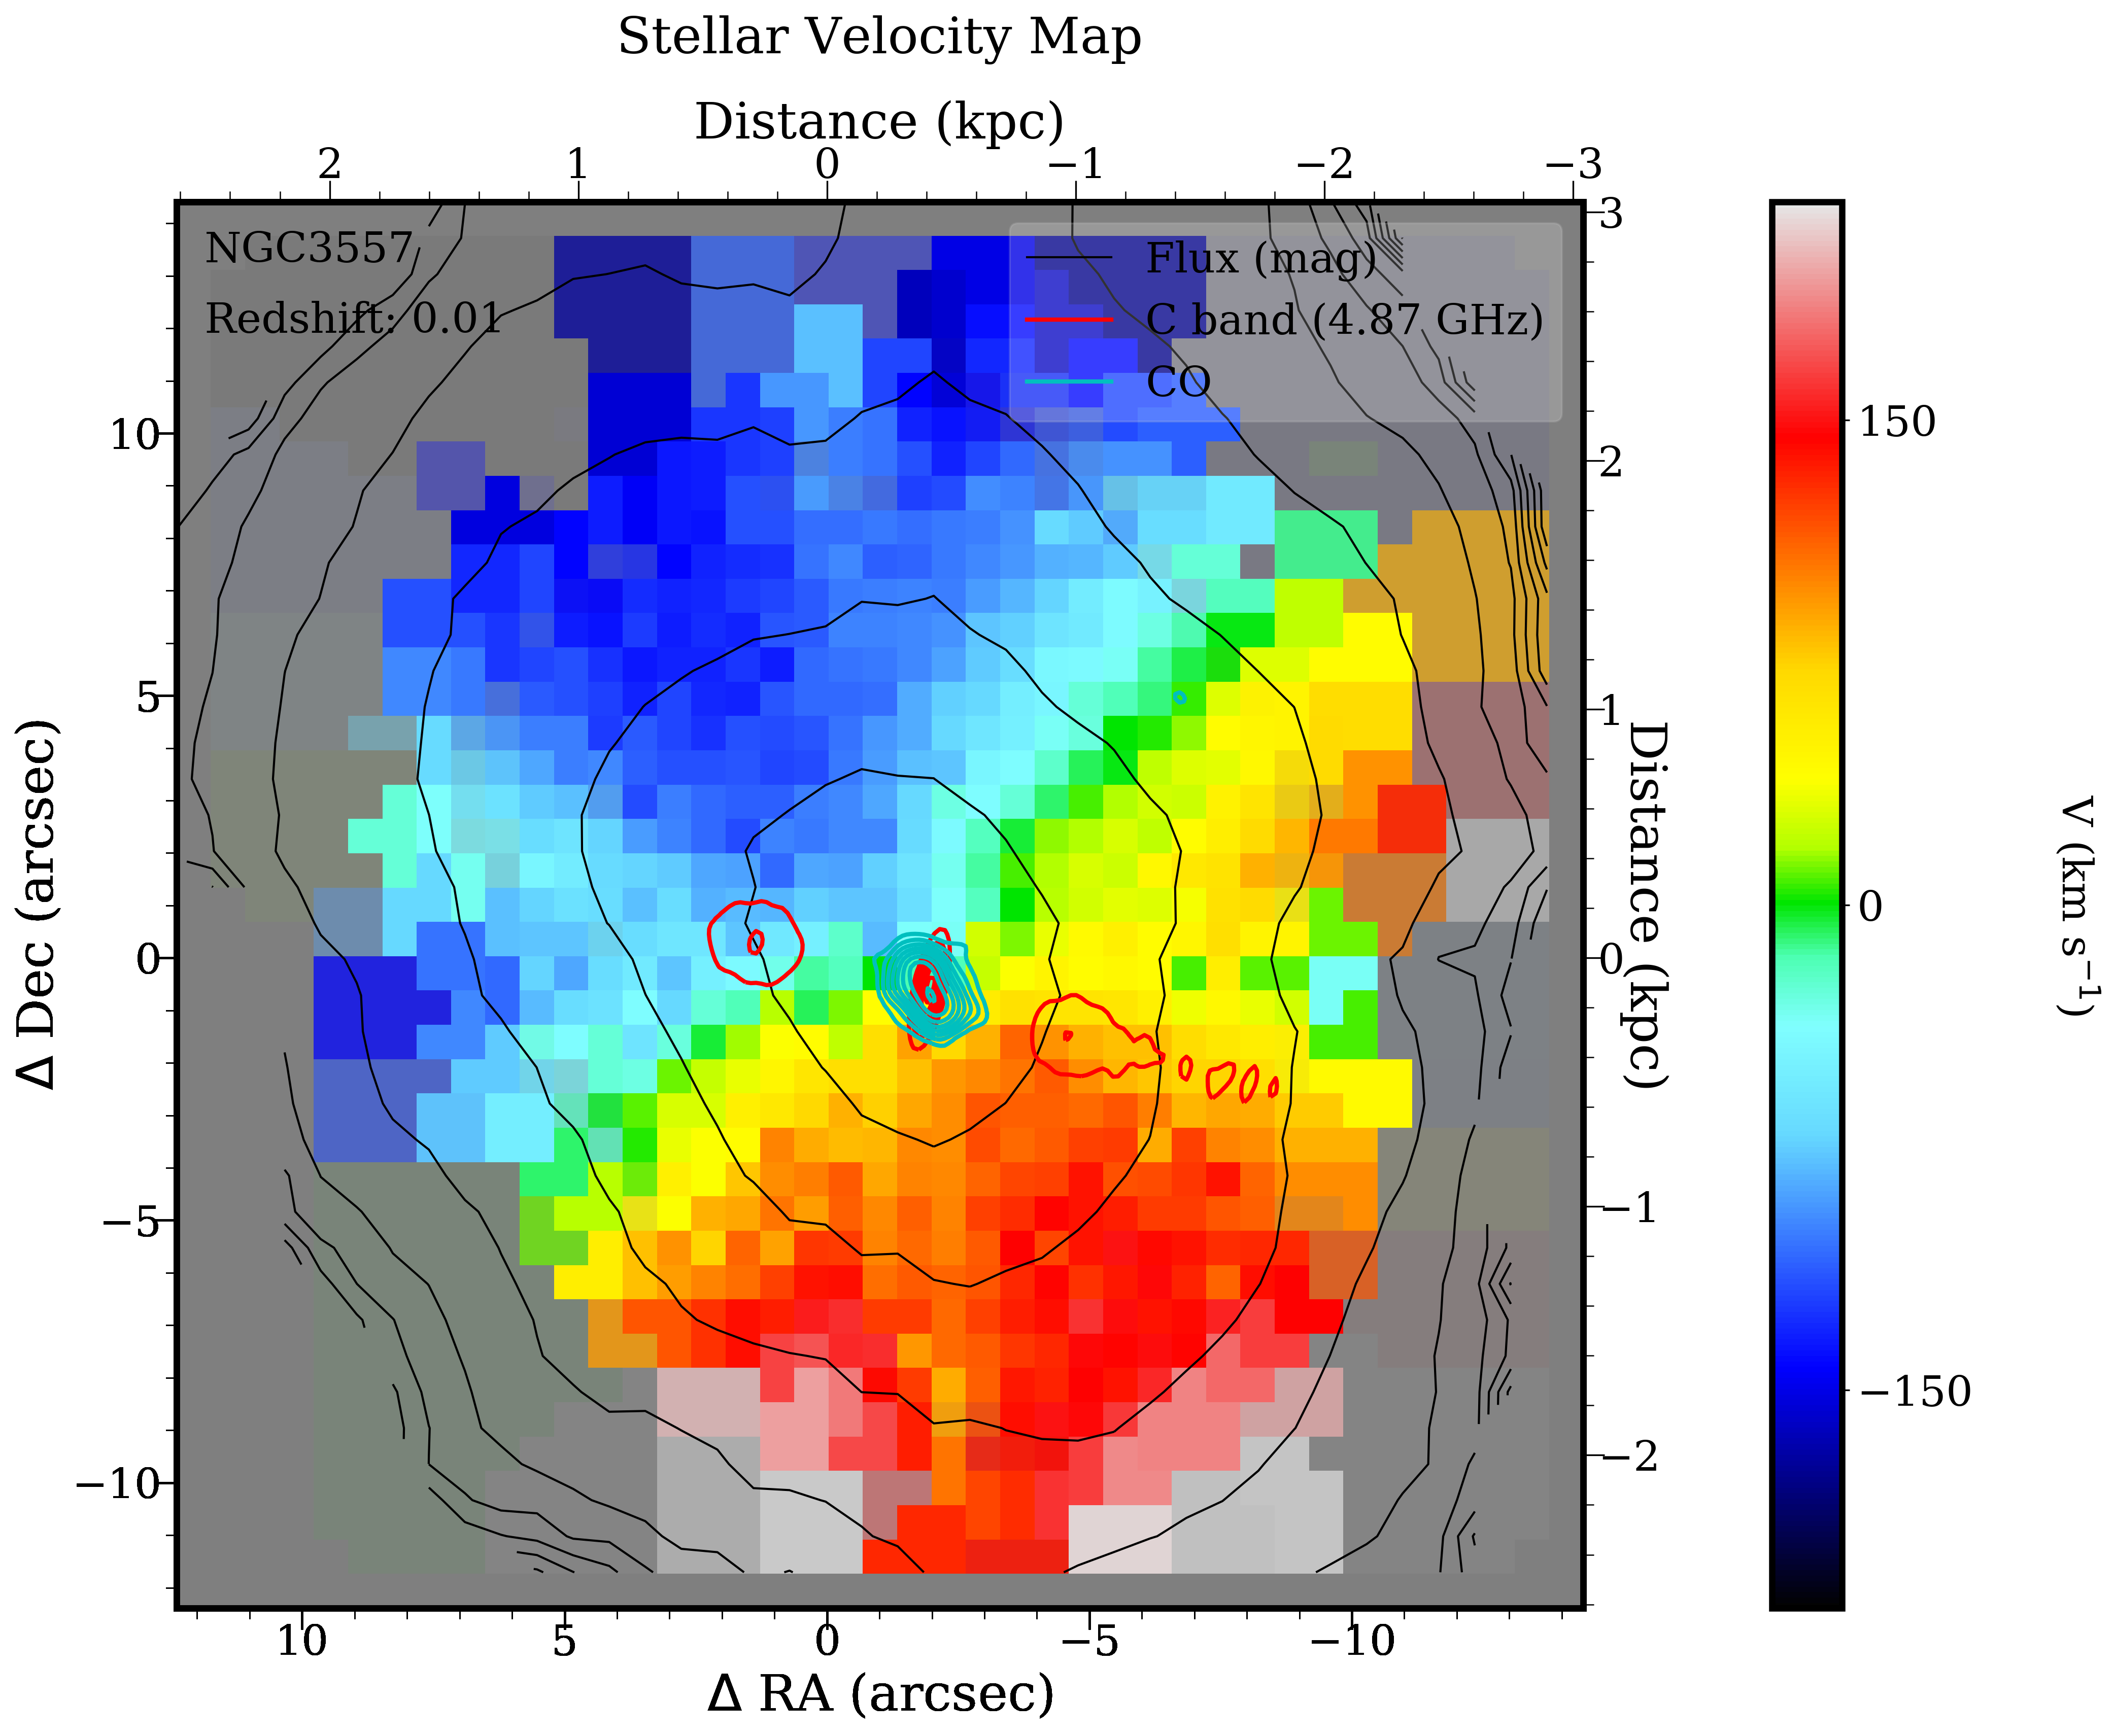
\includegraphics[width=0.245\textwidth]{Vmaps/ngc3557_stellar_vel.png}
      \includegraphics[width=0.245\textwidth]{Vmaps/ngc3100_stellar_vel.png}
      \includegraphics[width=0.245\textwidth]{Vmaps/ic1459_stellar_vel.png}
      \includegraphics[width=0.245\textwidth]{Vmaps/pks0718-34_stellar_vel.png}
      \includegraphics[width=0.245\textwidth]{Vmaps/ic4296_stellar_vel.png}
      \includegraphics[width=0.245\textwidth]{Vmaps/ngc7075_stellar_vel.png}
      \includegraphics[width=0.245\textwidth]{Vmaps/ic1531_stellar_vel.png}
      \includegraphics[width=0.245\textwidth]{Vmaps/ngc1399_stellar_vel.png}
      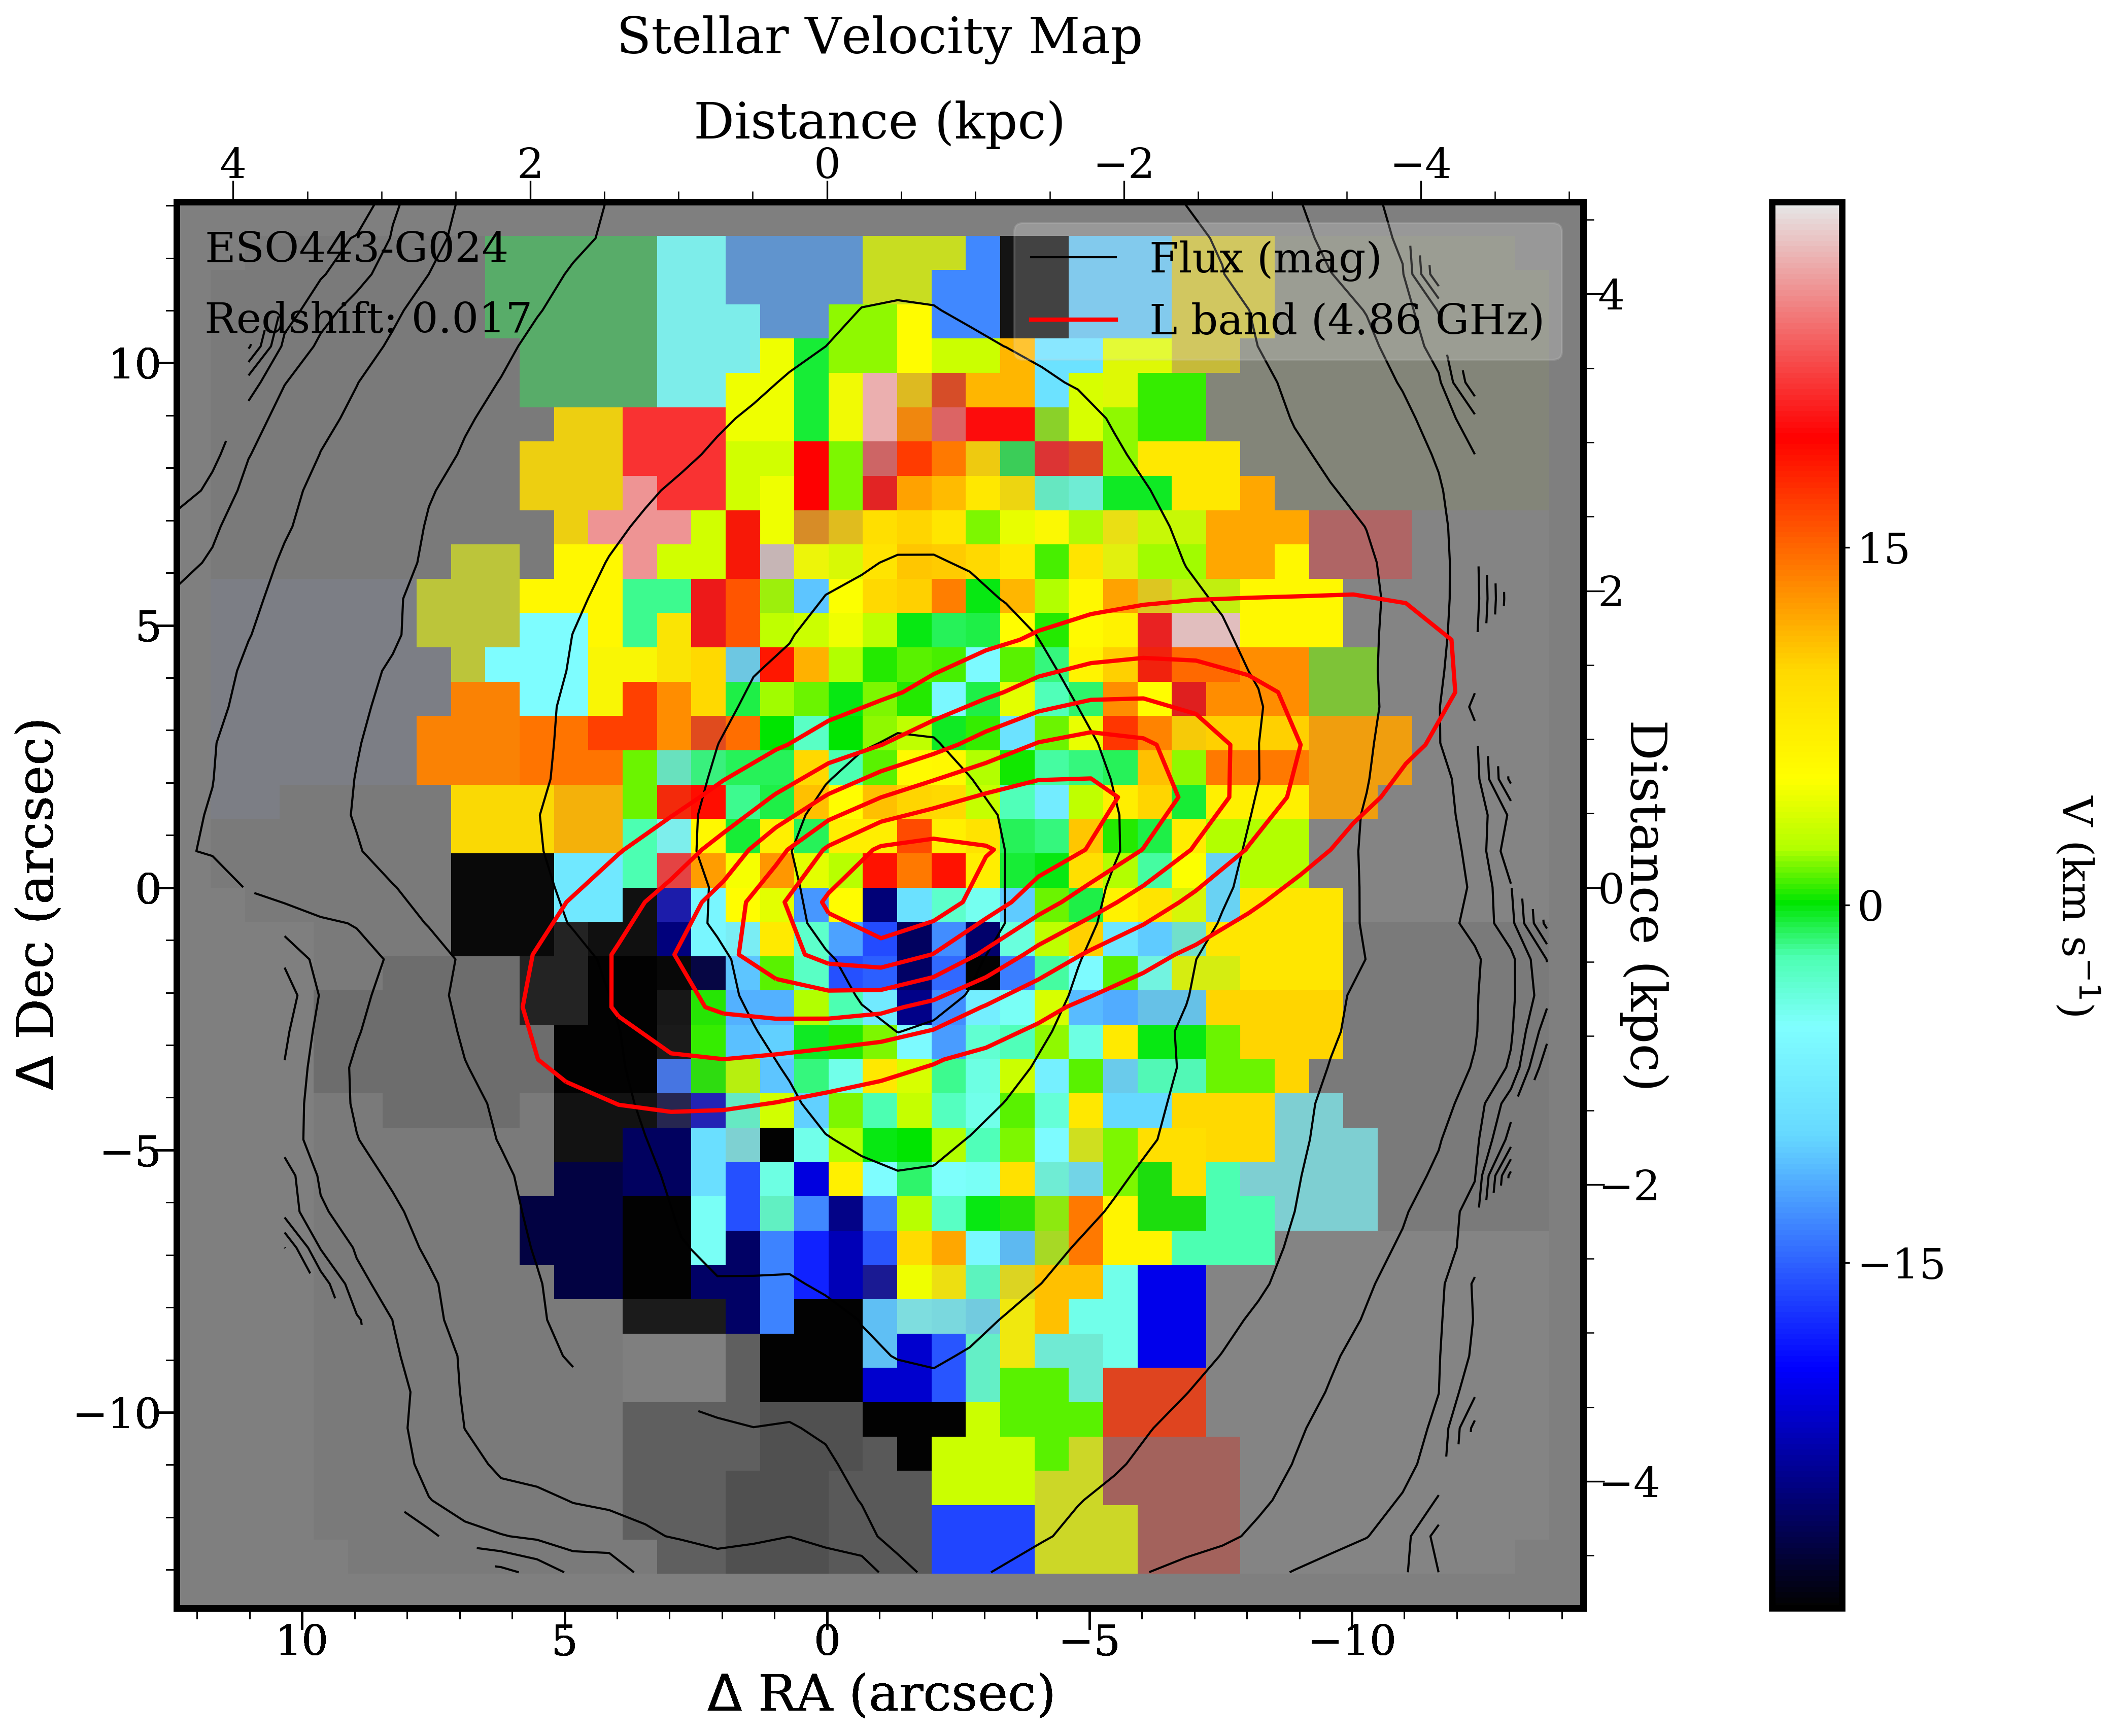
\includegraphics[width=0.245\textwidth]{Vmaps/eso443-g024_stellar_vel.png}
      \caption[VIMOS velocity maps]{Velocity for each galaxy in the VIMOS sample. Plots are ordered and contour colors are as in figure \ref{fig:Vstellar_img}}
      \label{fig:Vstellar_vel}
\end{figure*}

\begin{figure*}
      \centering
      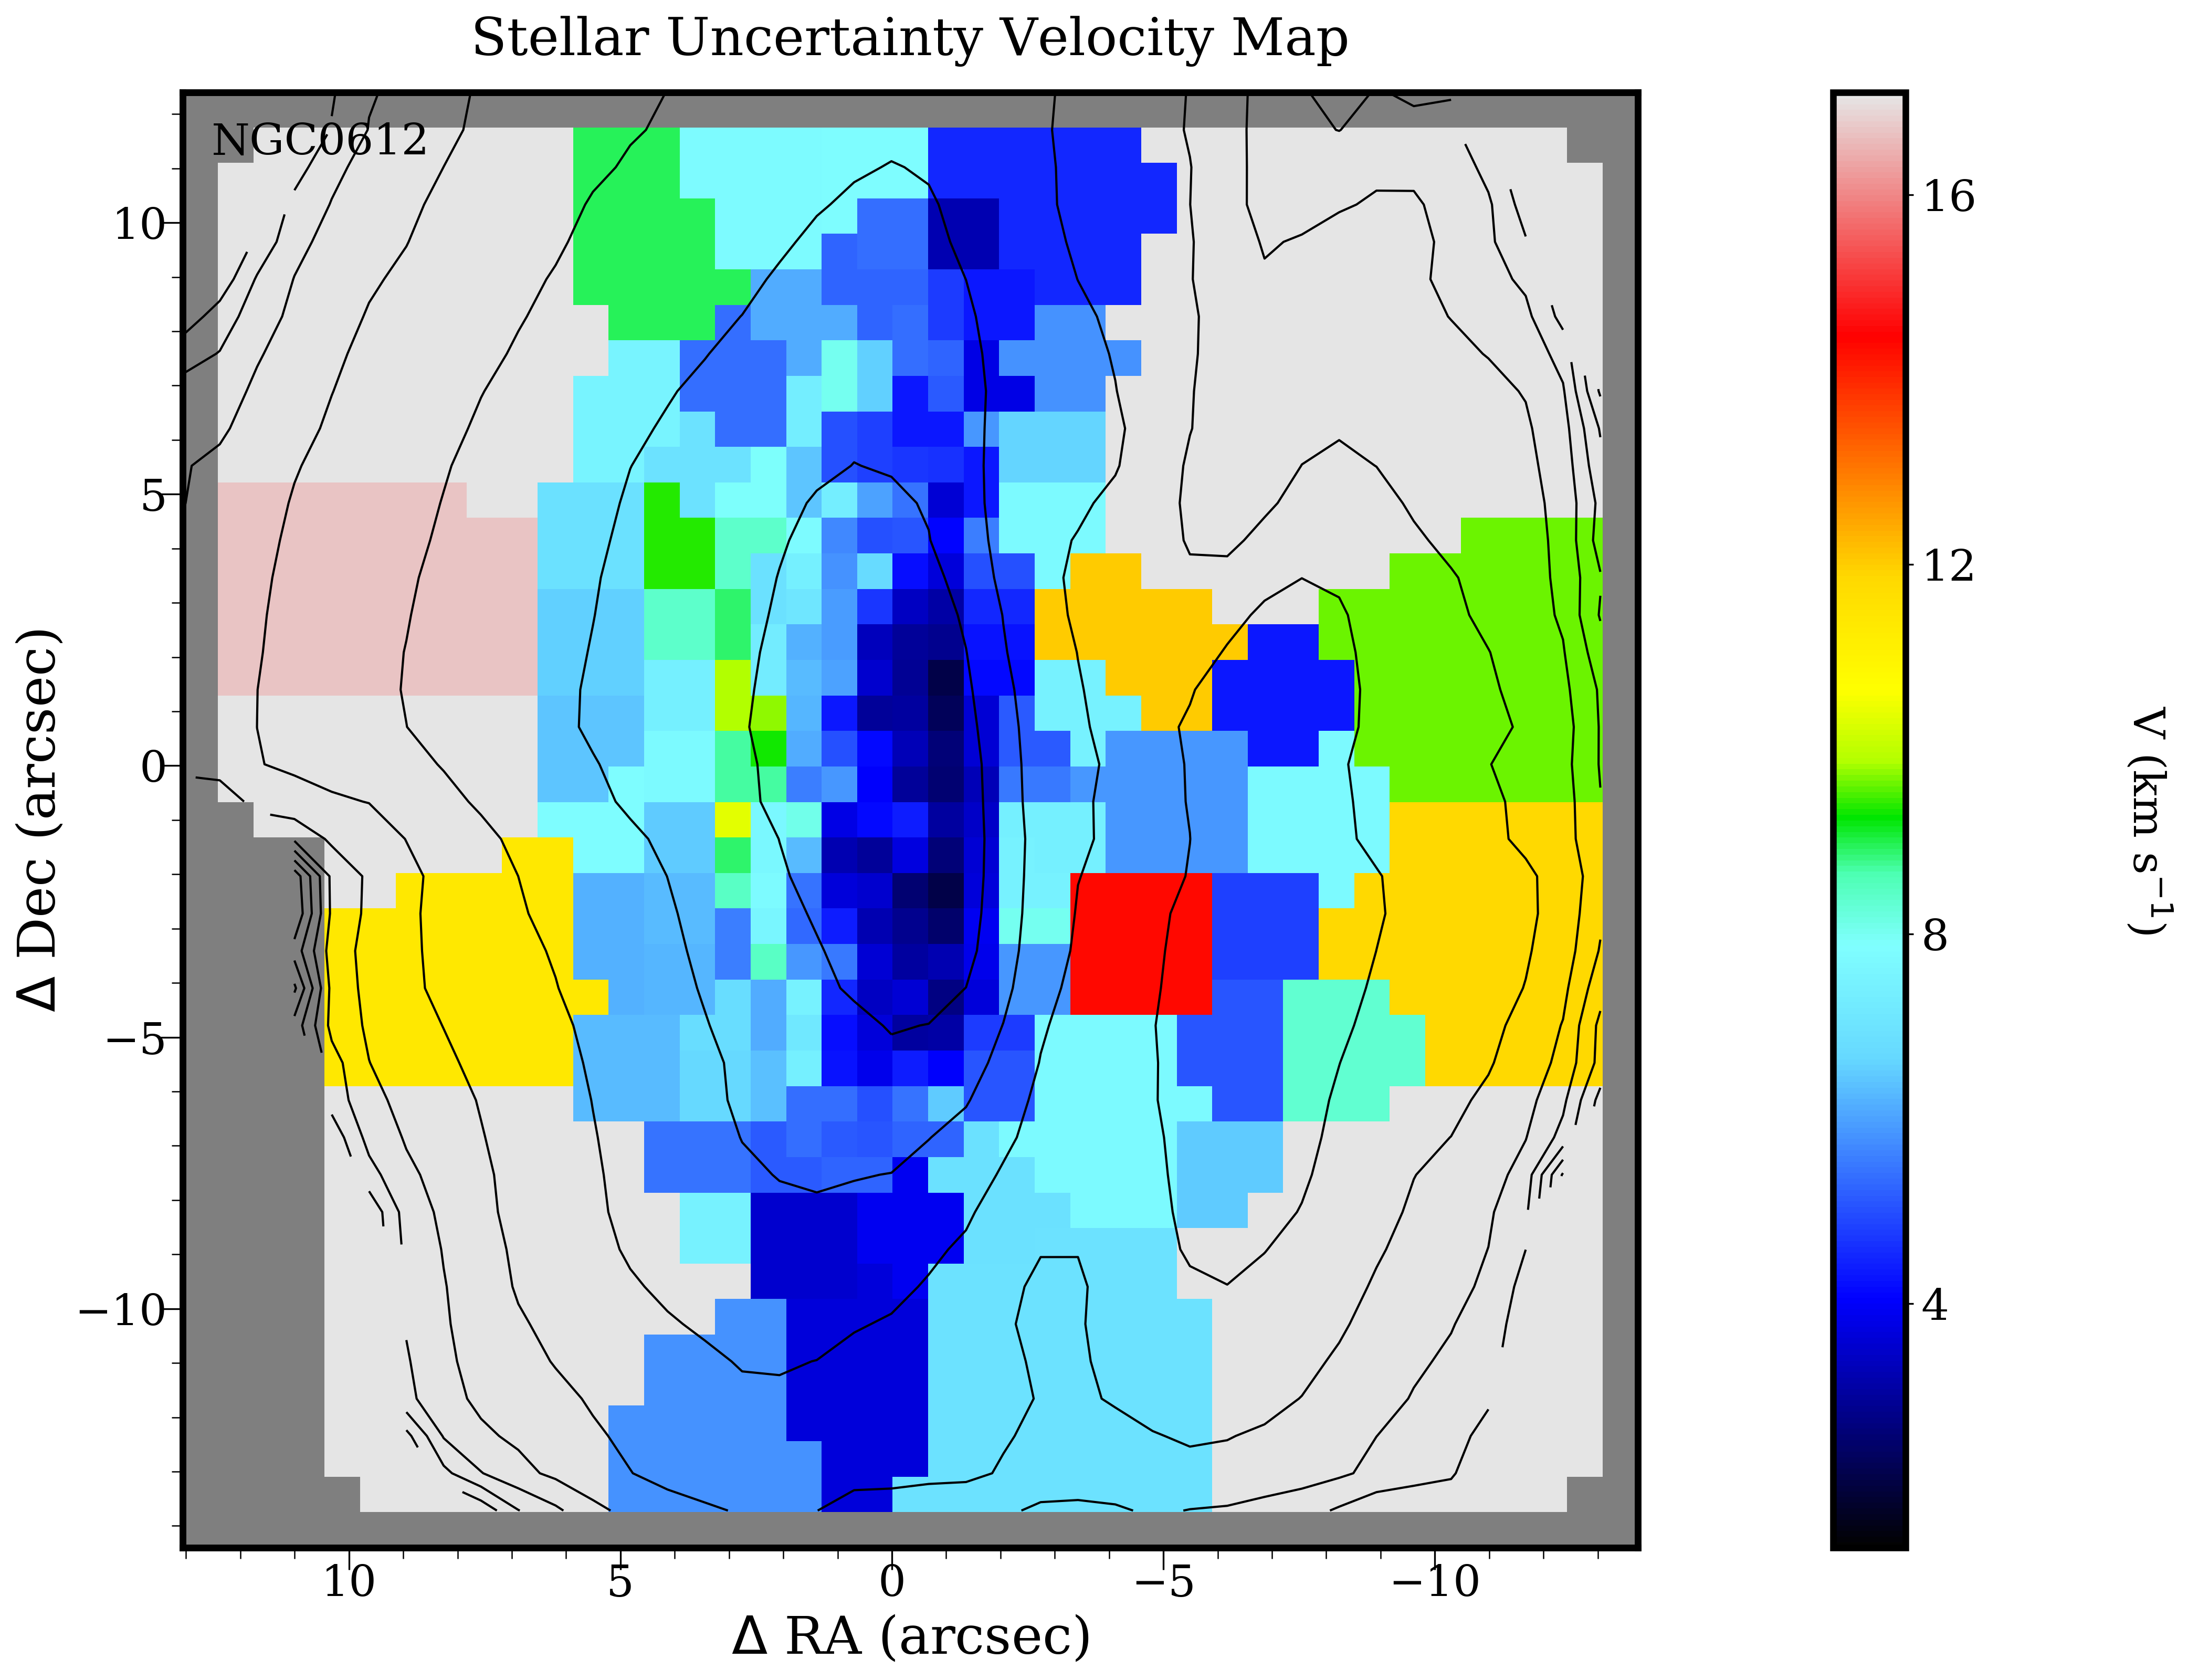
\includegraphics[width=0.245\textwidth]{Vmaps/ngc0612_stellar_vel_uncert.png}
      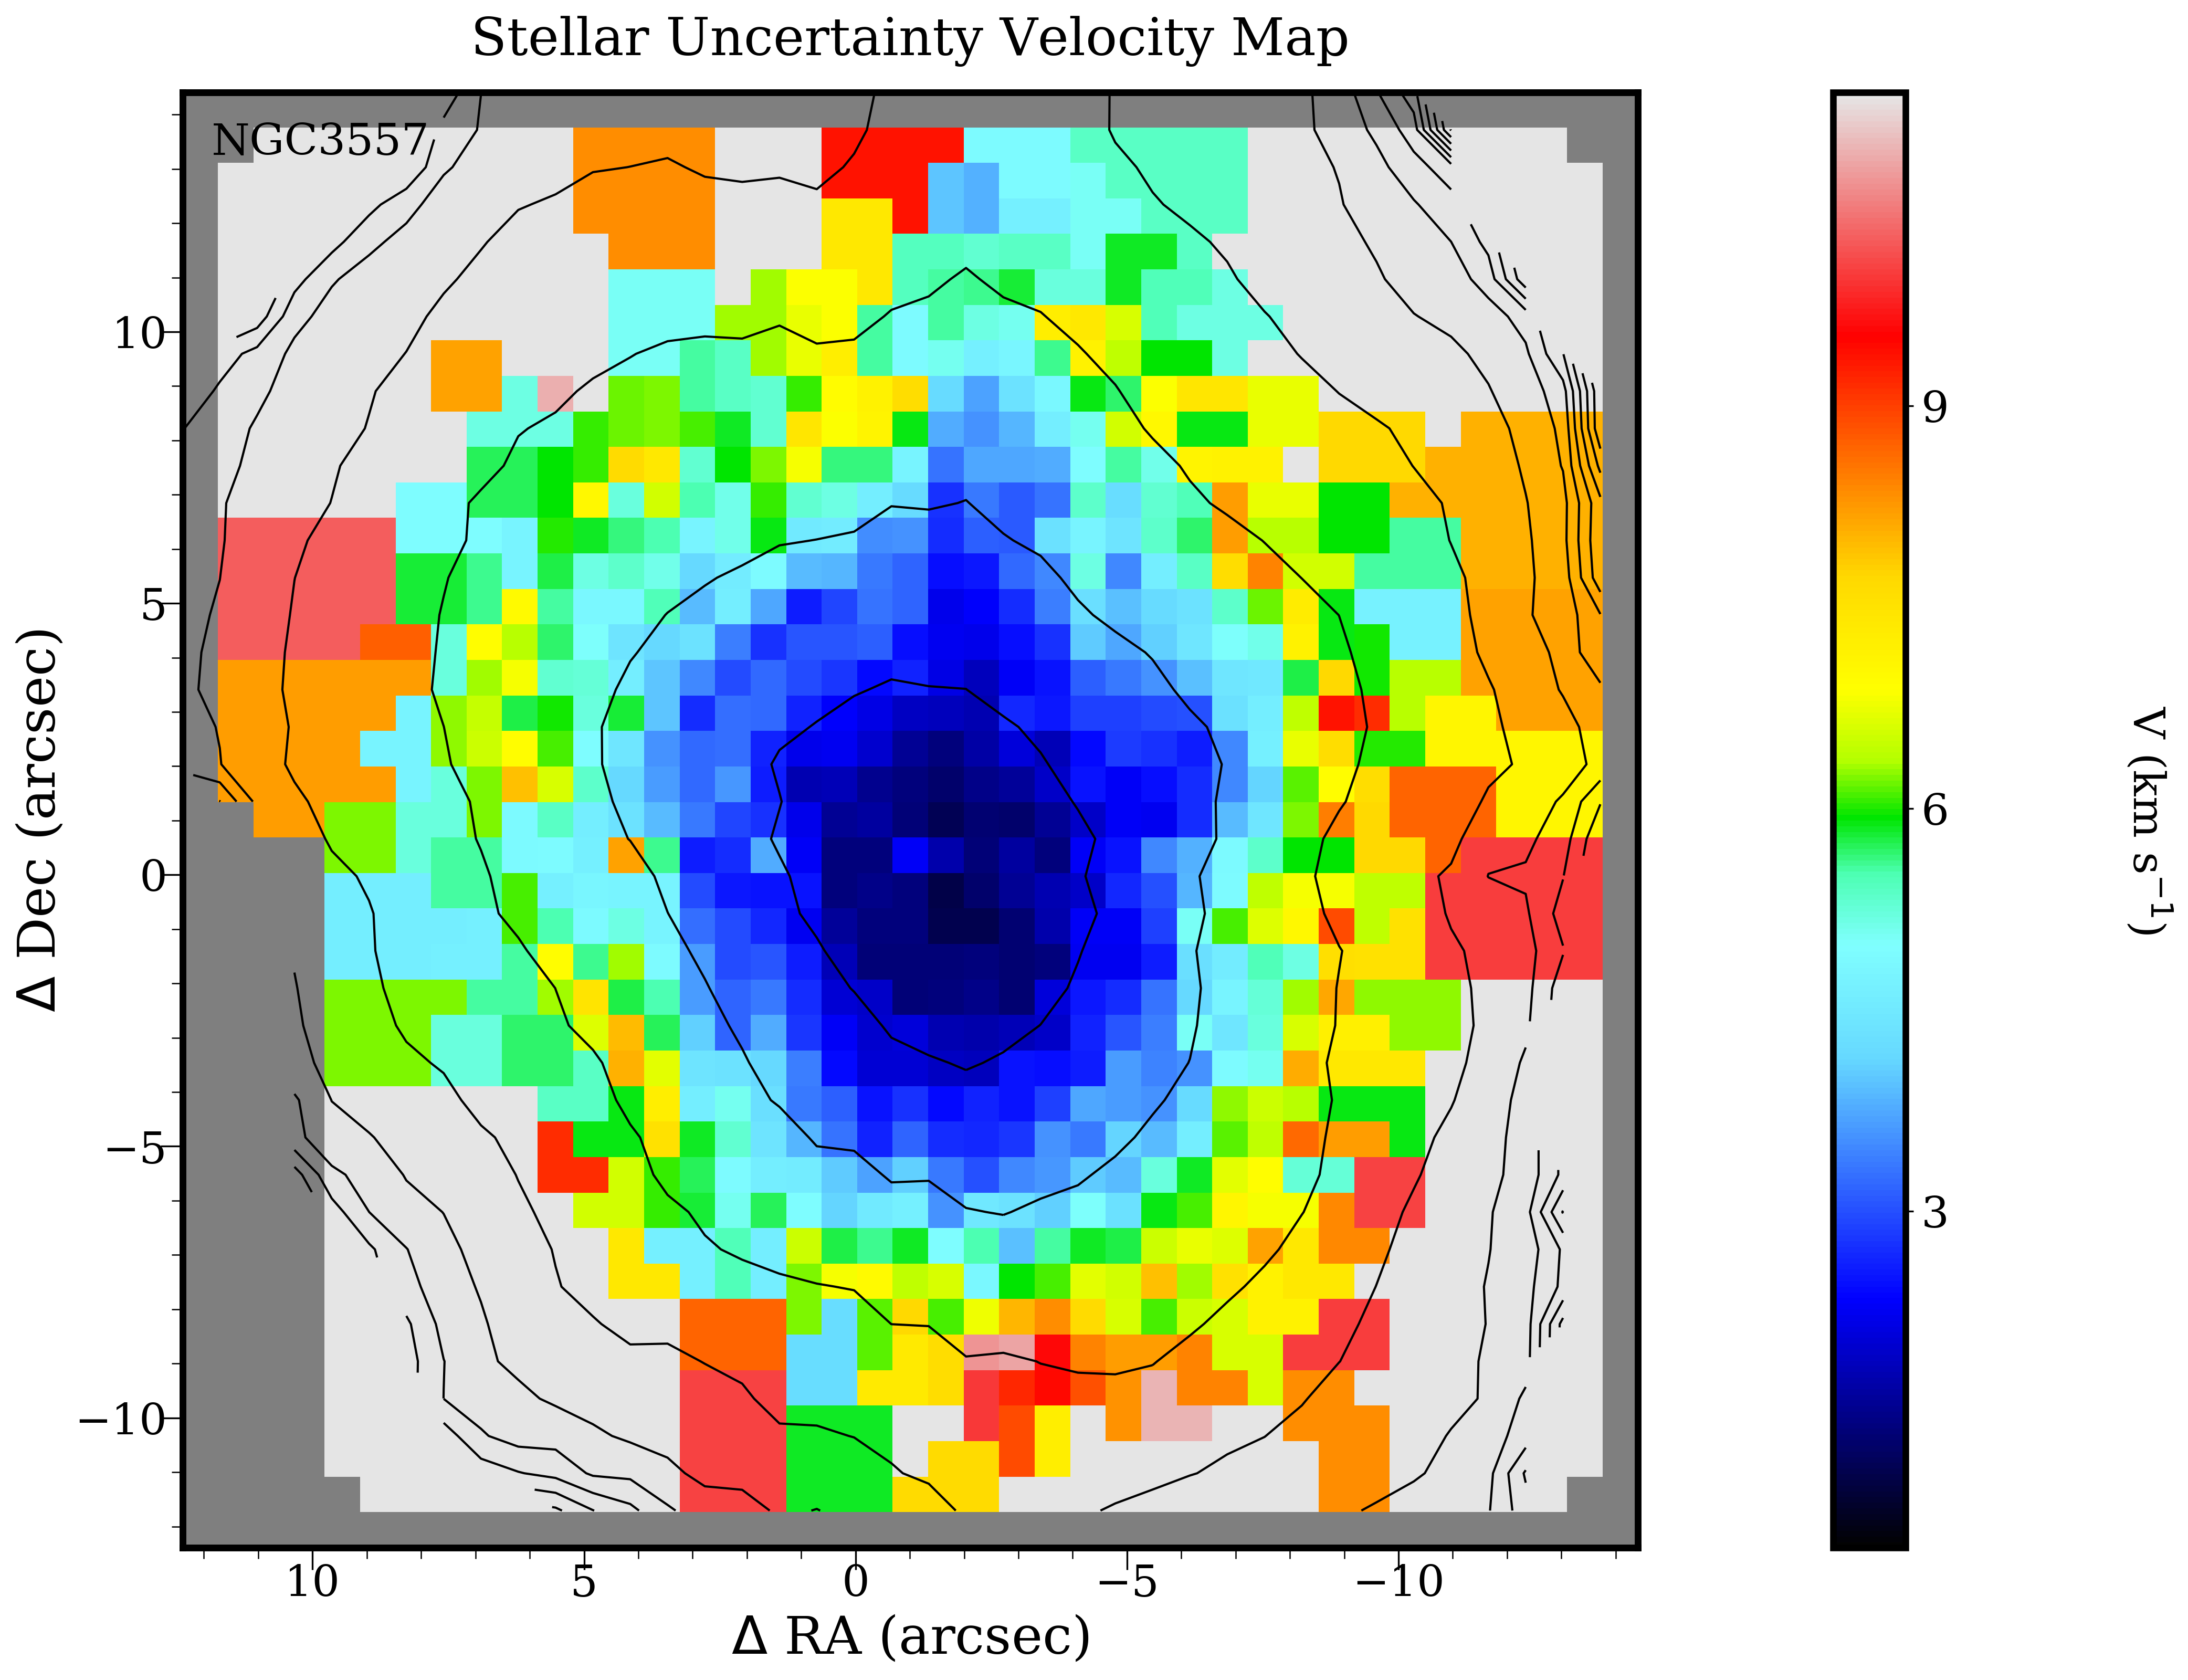
\includegraphics[width=0.245\textwidth]{Vmaps/ngc3557_stellar_vel_uncert.png}
      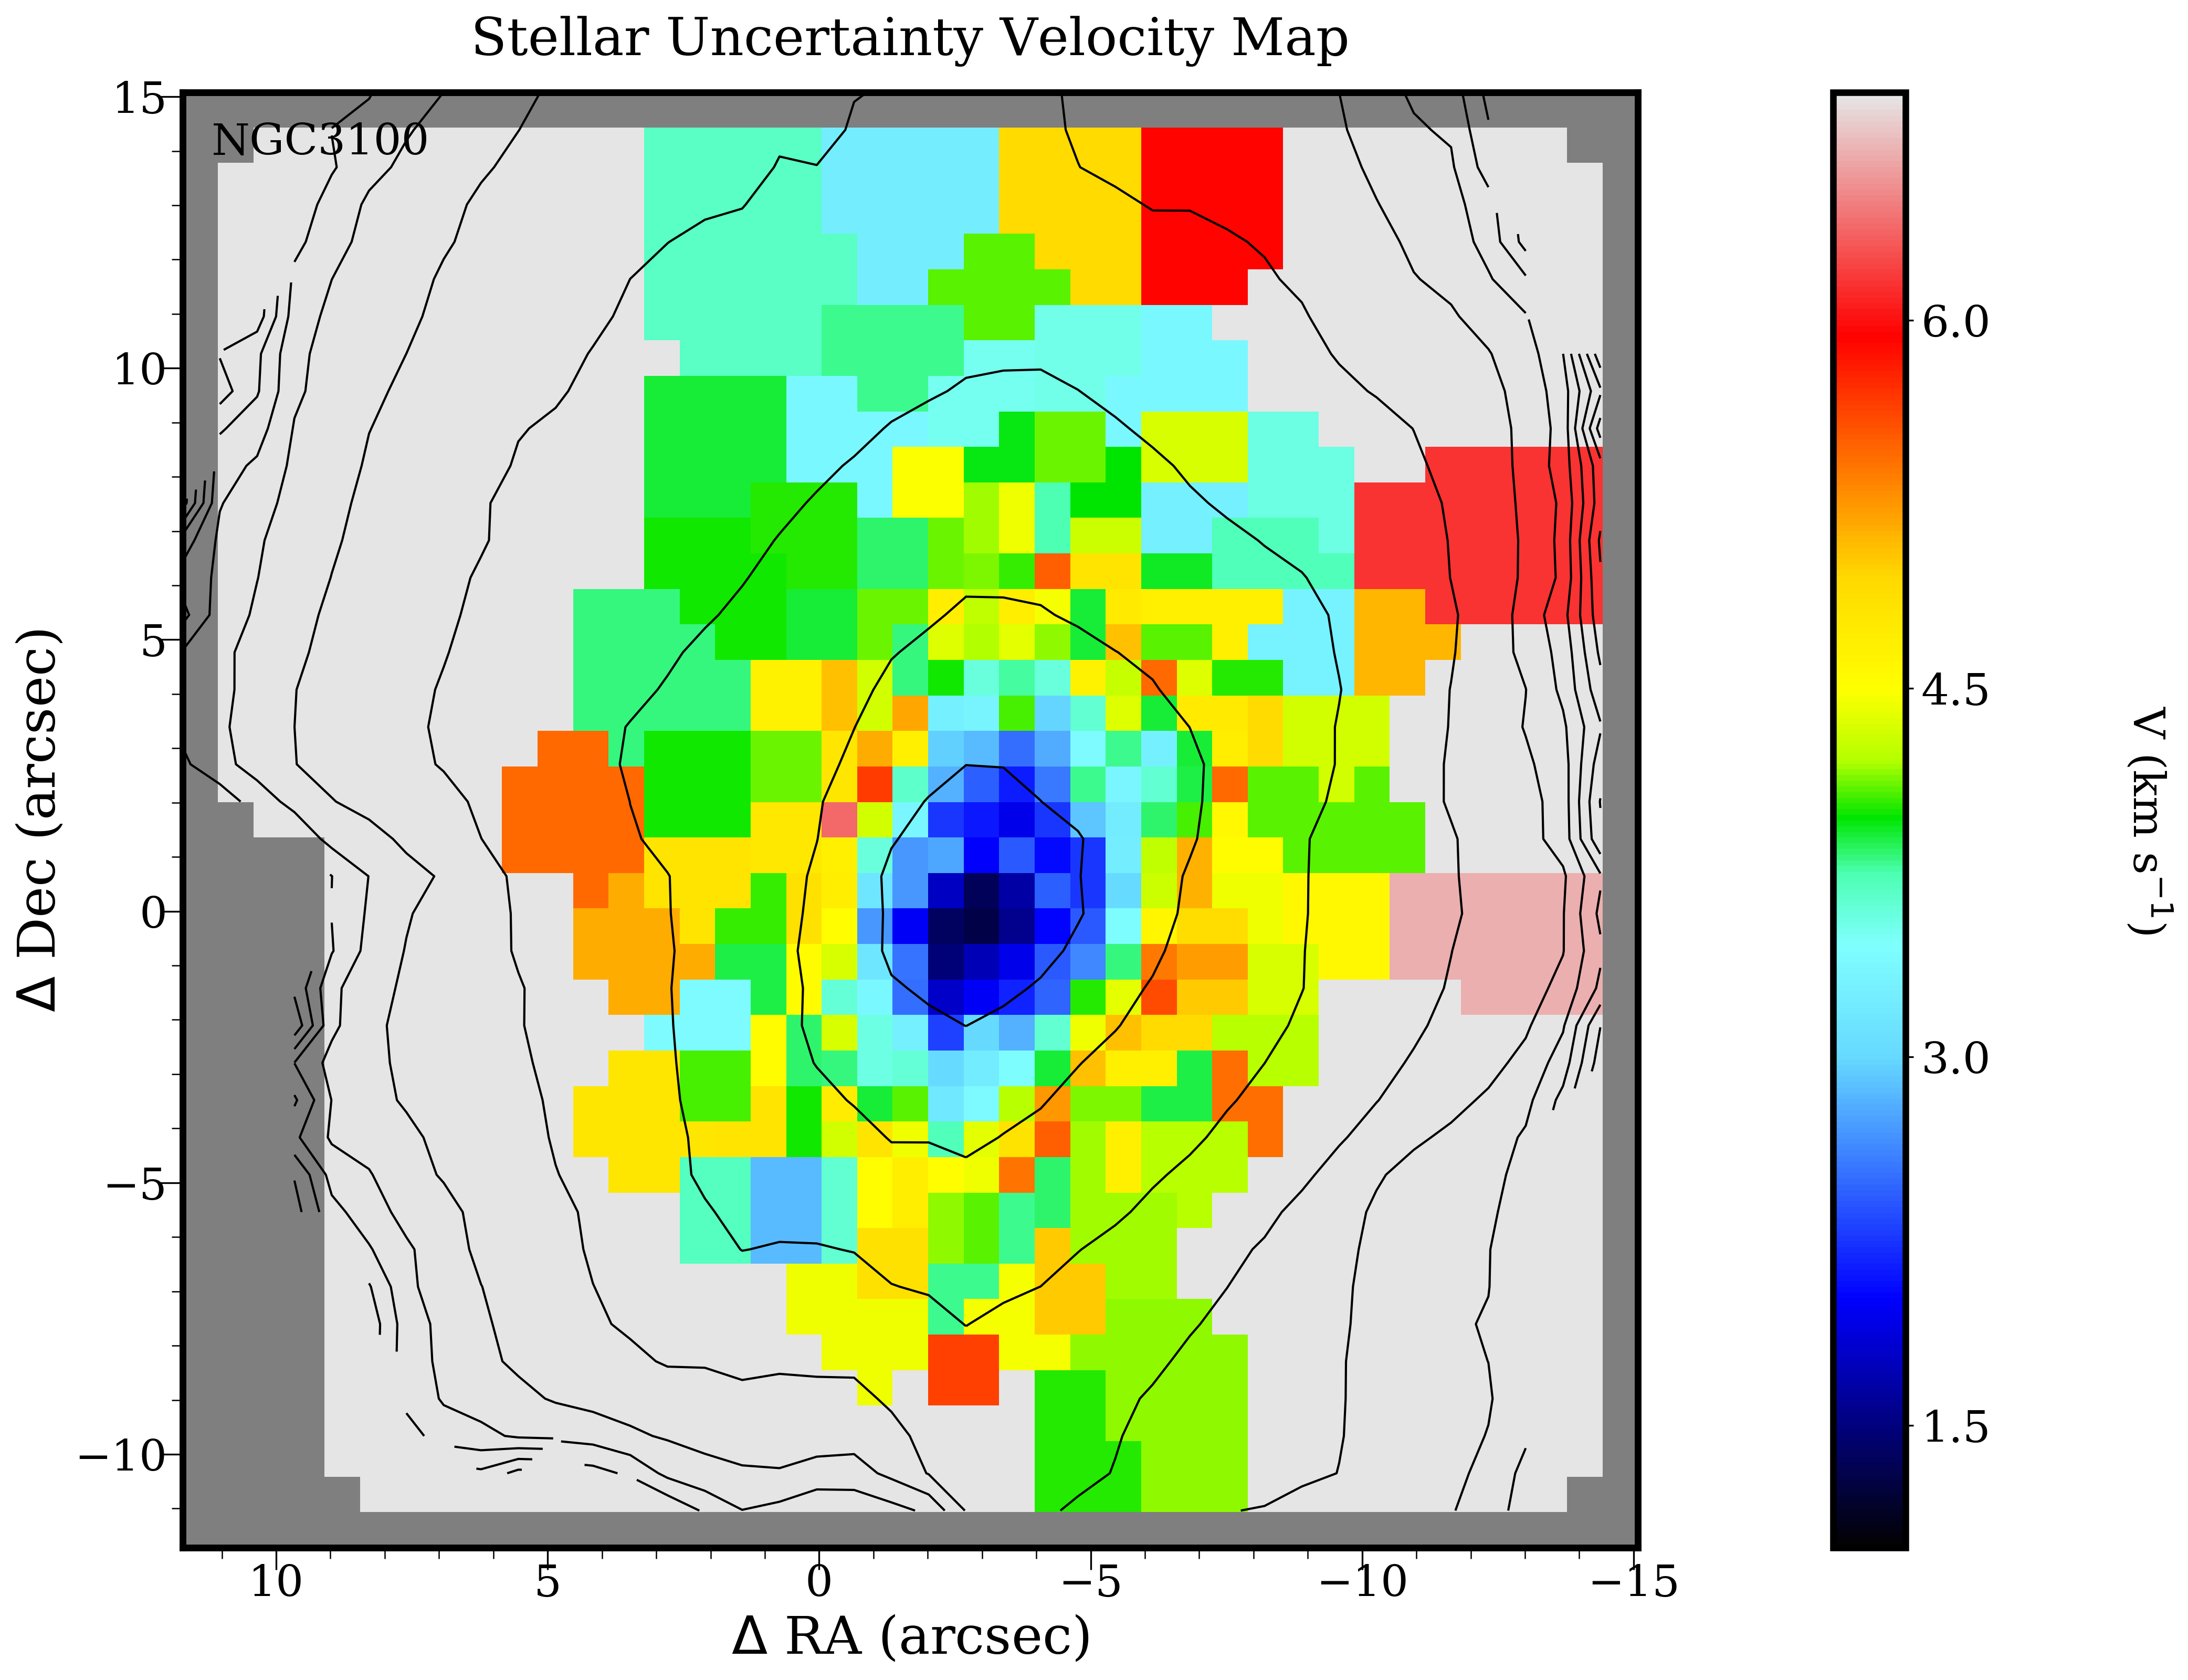
\includegraphics[width=0.245\textwidth]{Vmaps/ngc3100_stellar_vel_uncert.png}
      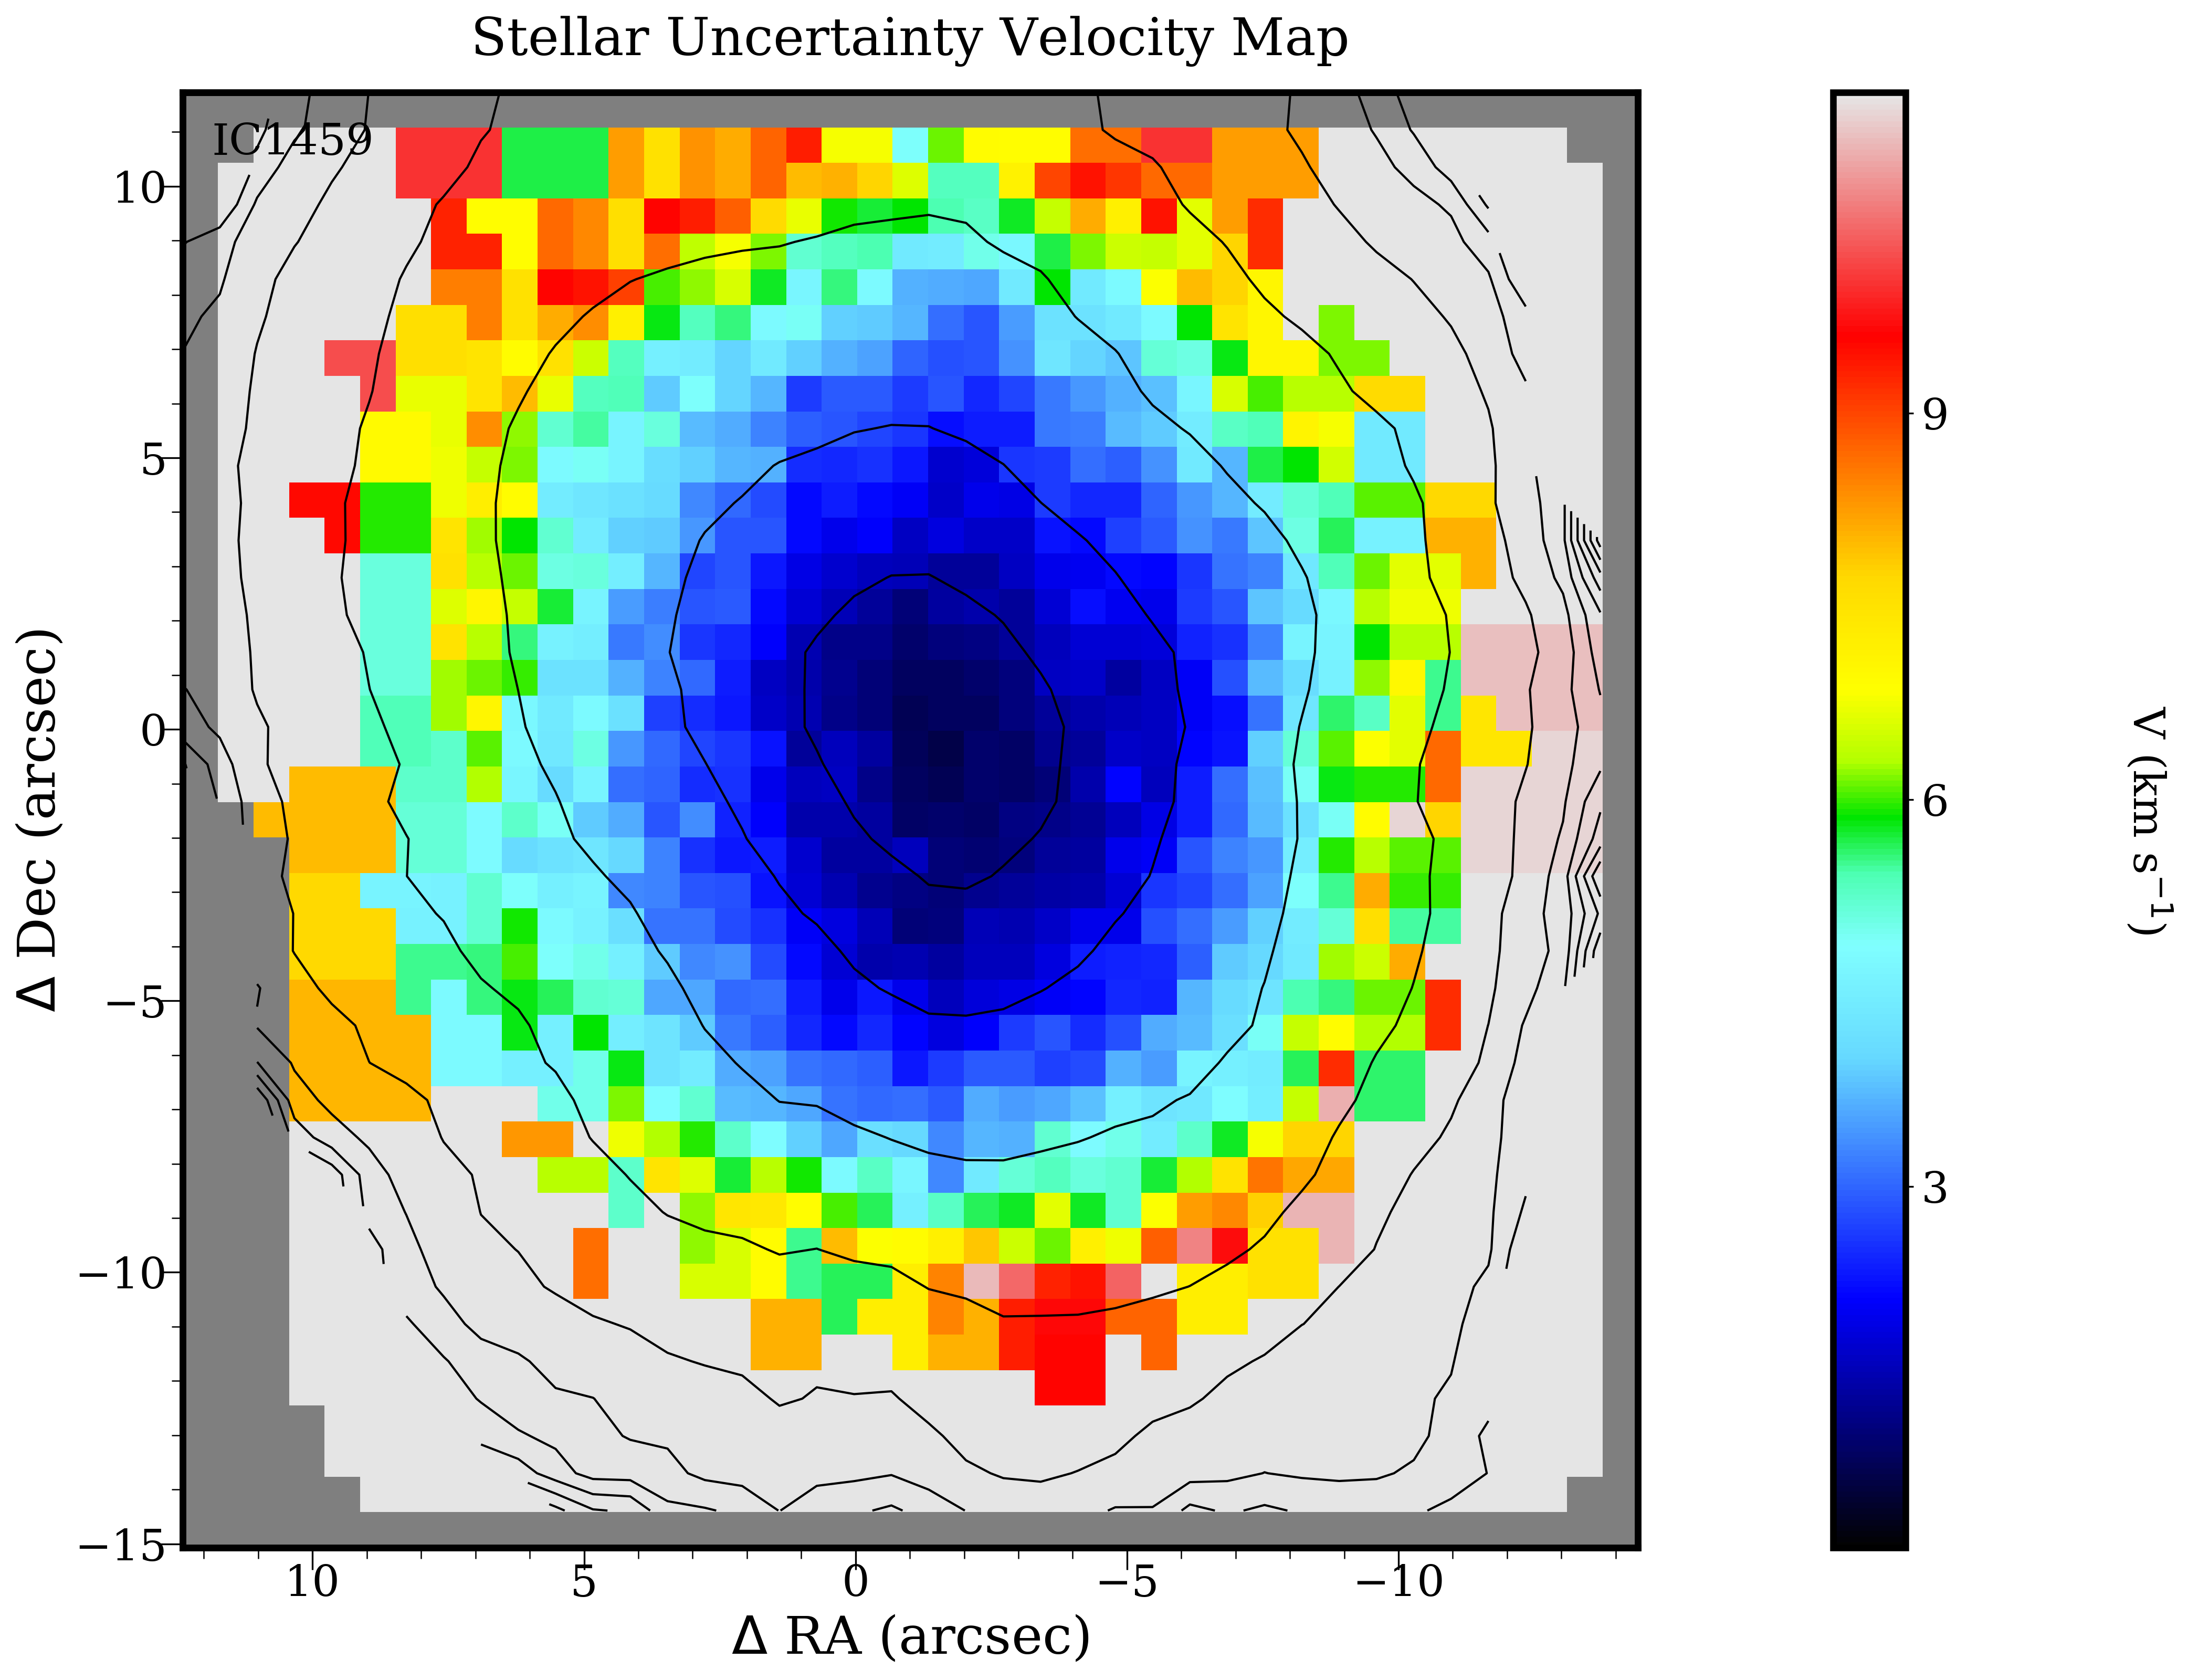
\includegraphics[width=0.245\textwidth]{Vmaps/ic1459_stellar_vel_uncert.png}
      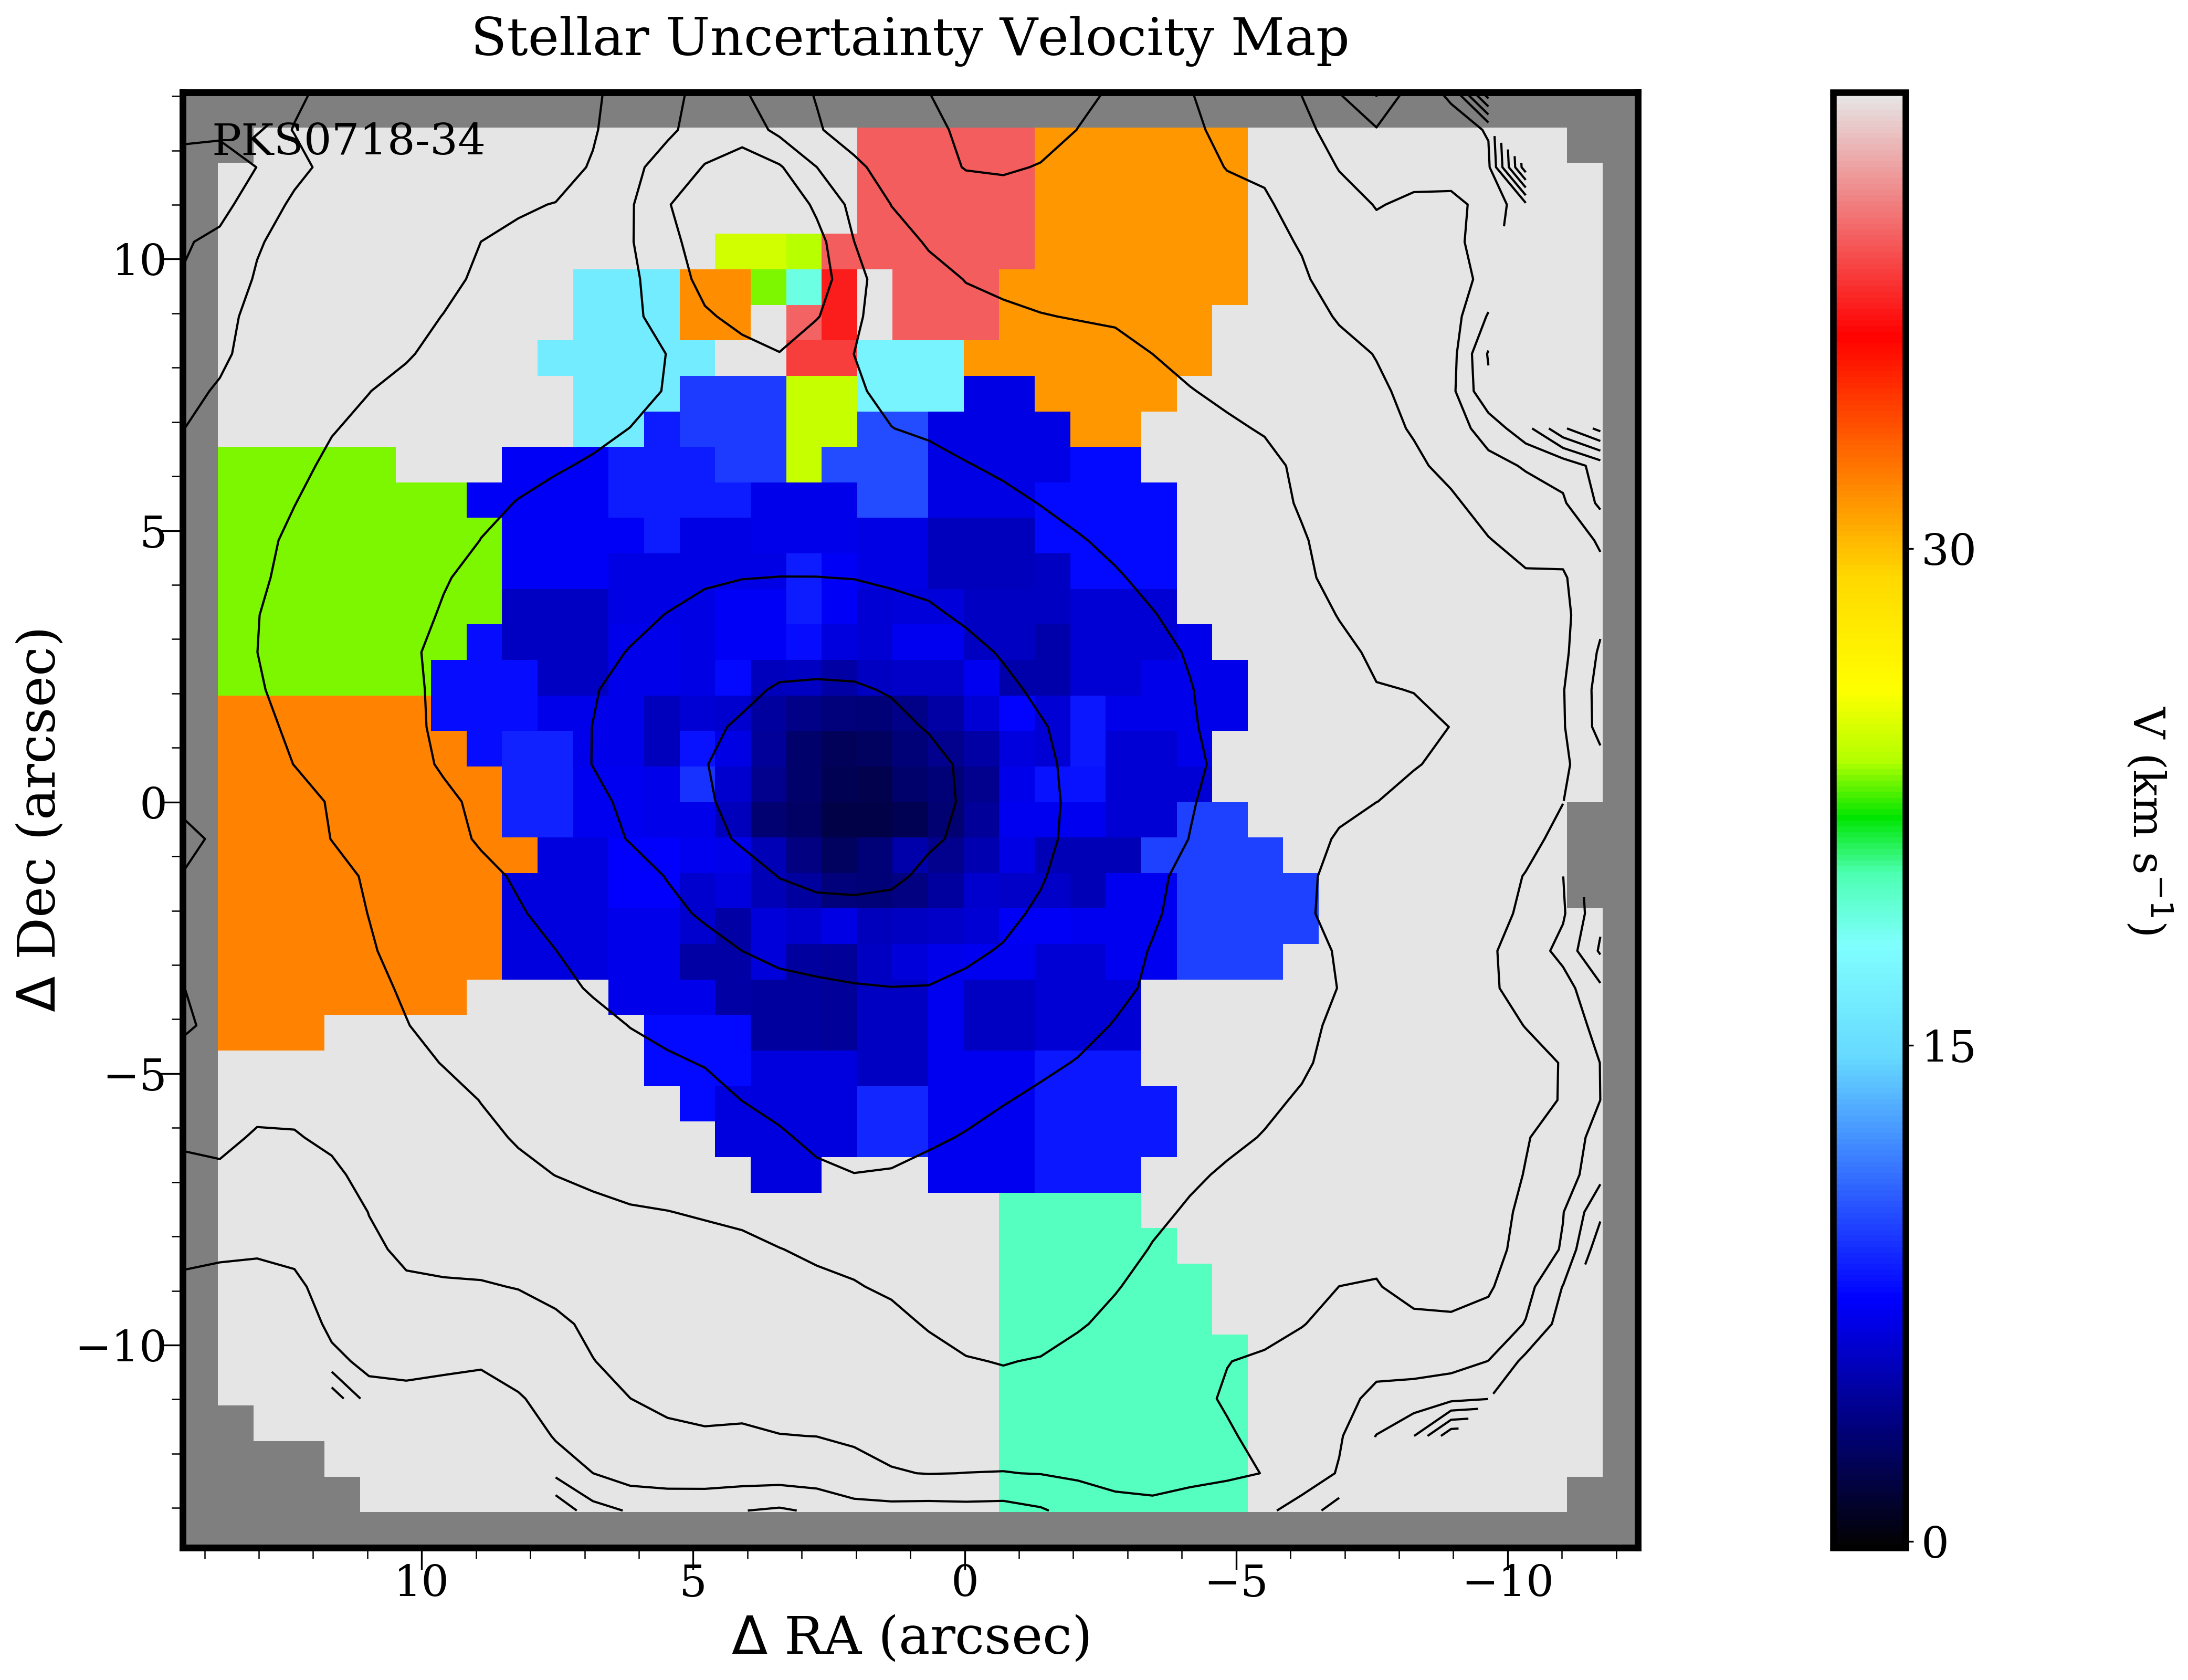
\includegraphics[width=0.245\textwidth]{Vmaps/pks0718-34_stellar_vel_uncert.png}
      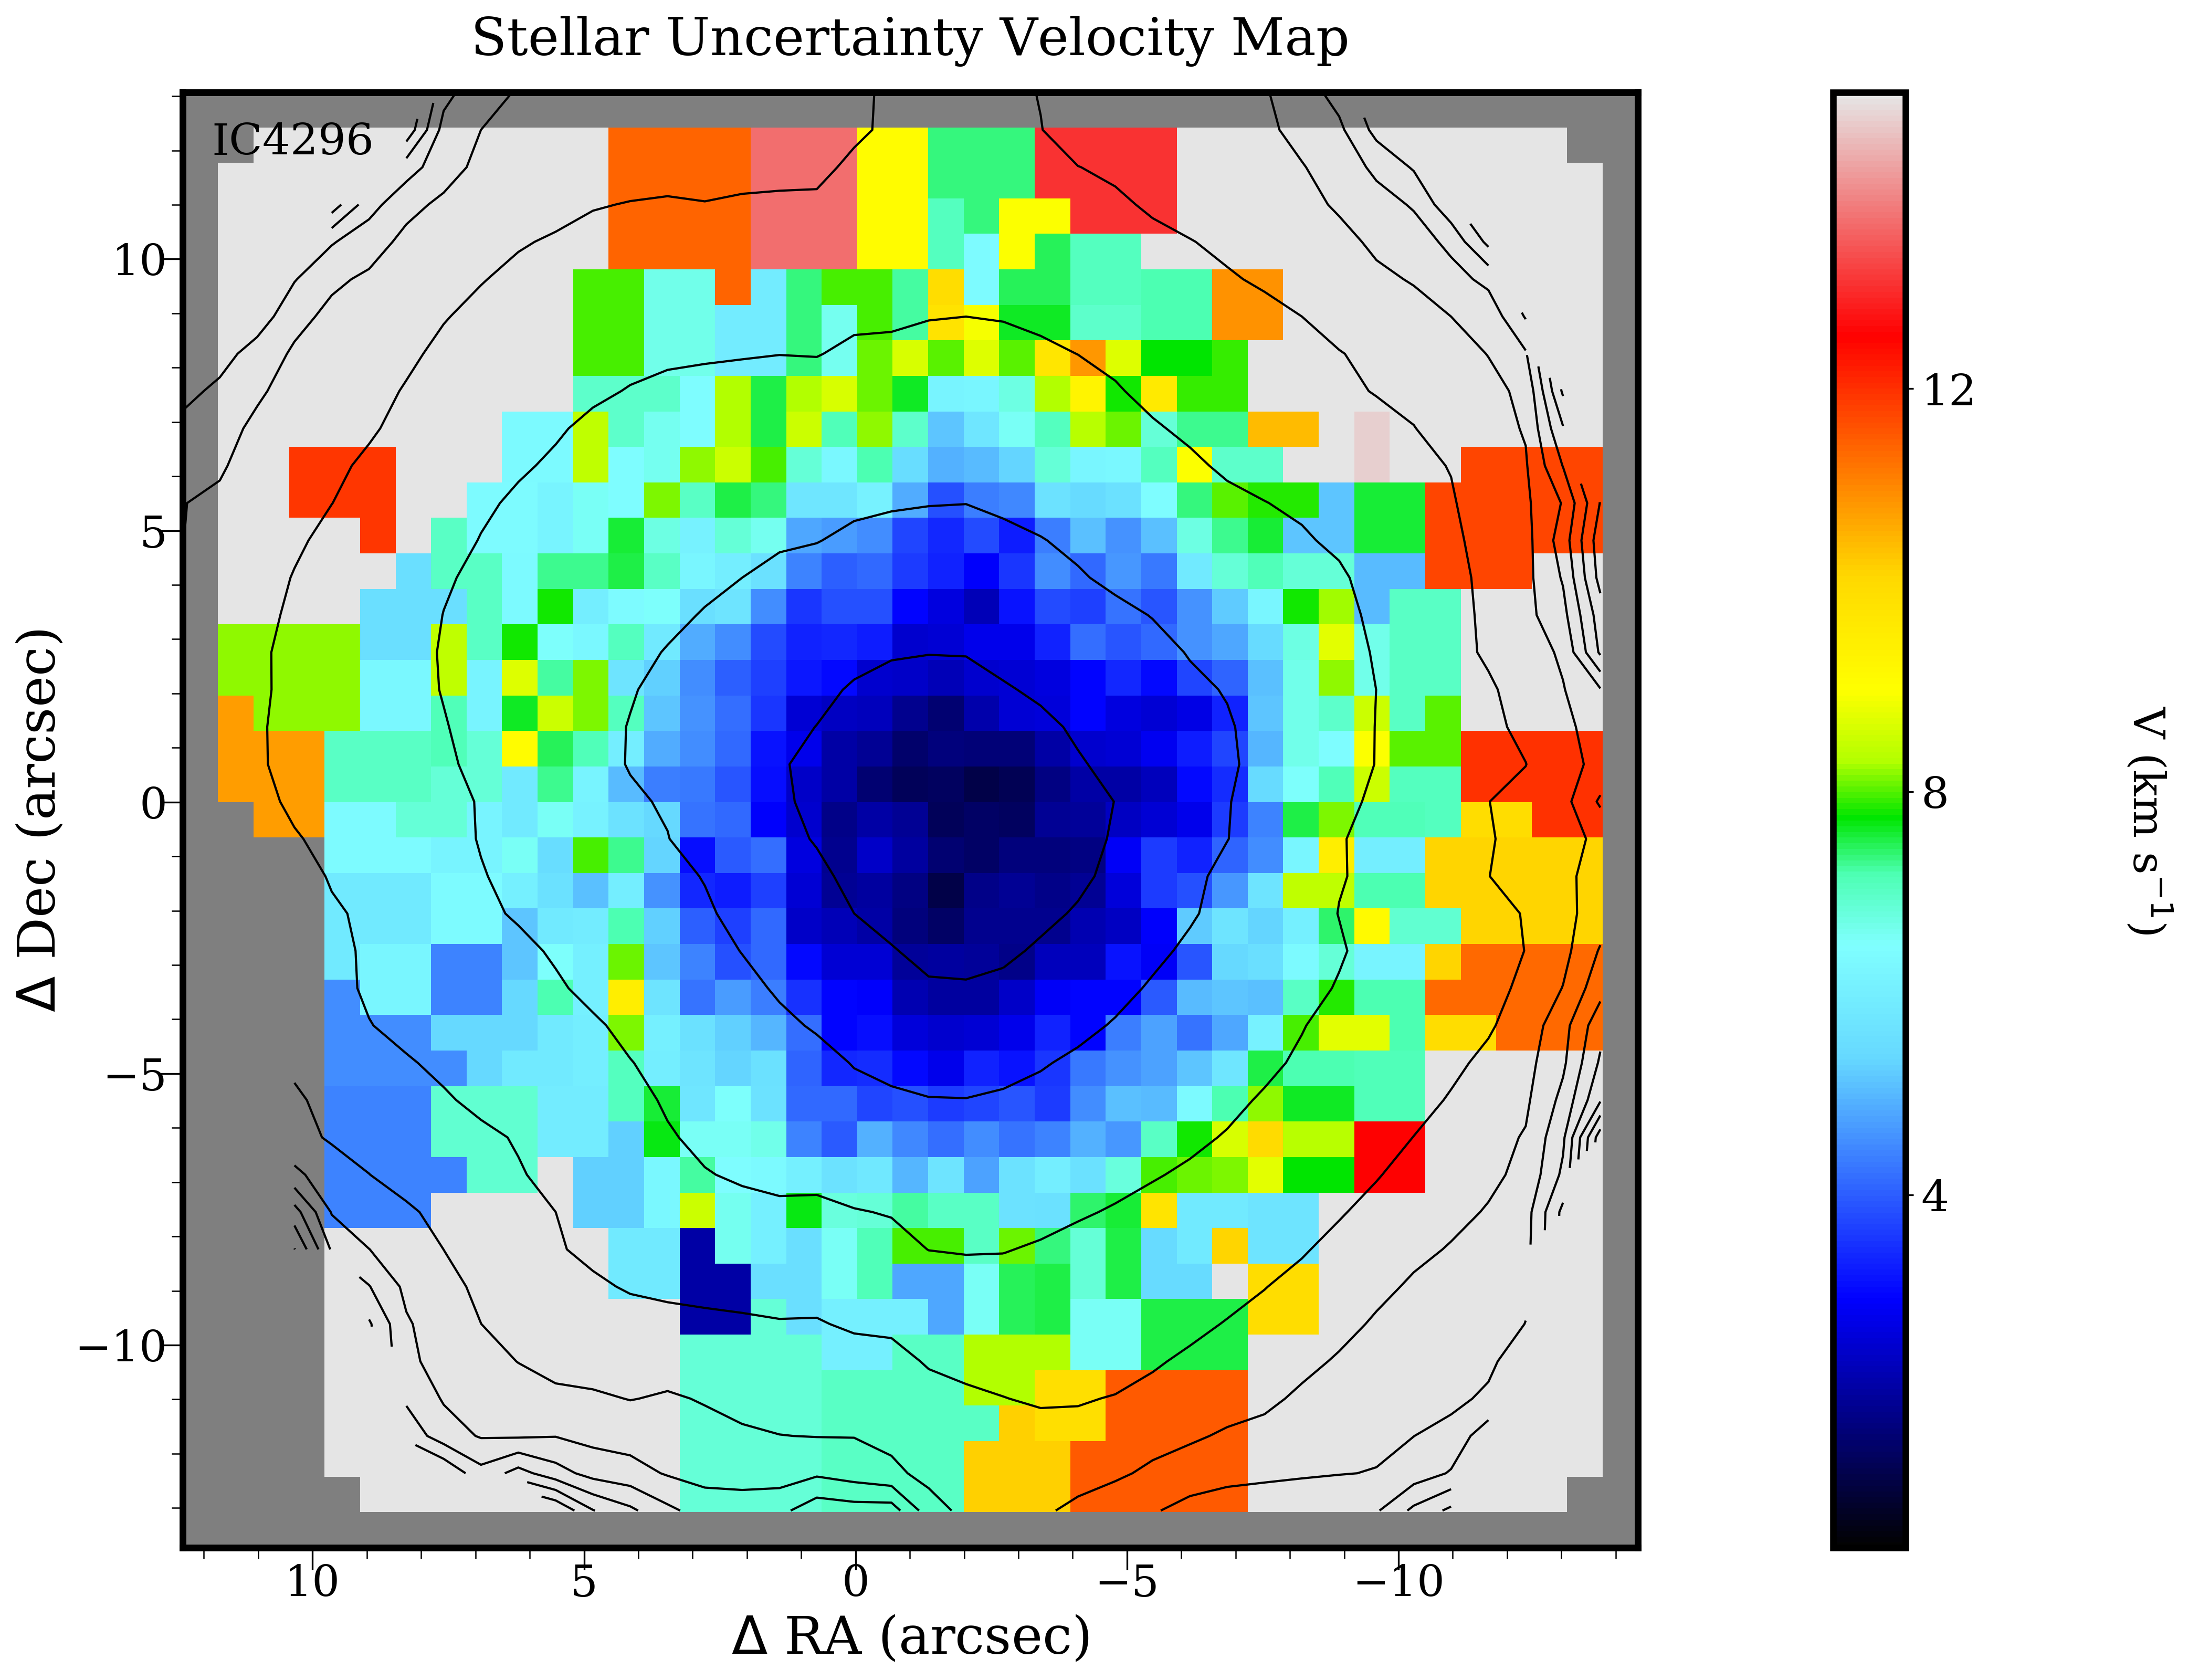
\includegraphics[width=0.245\textwidth]{Vmaps/ic4296_stellar_vel_uncert.png}
      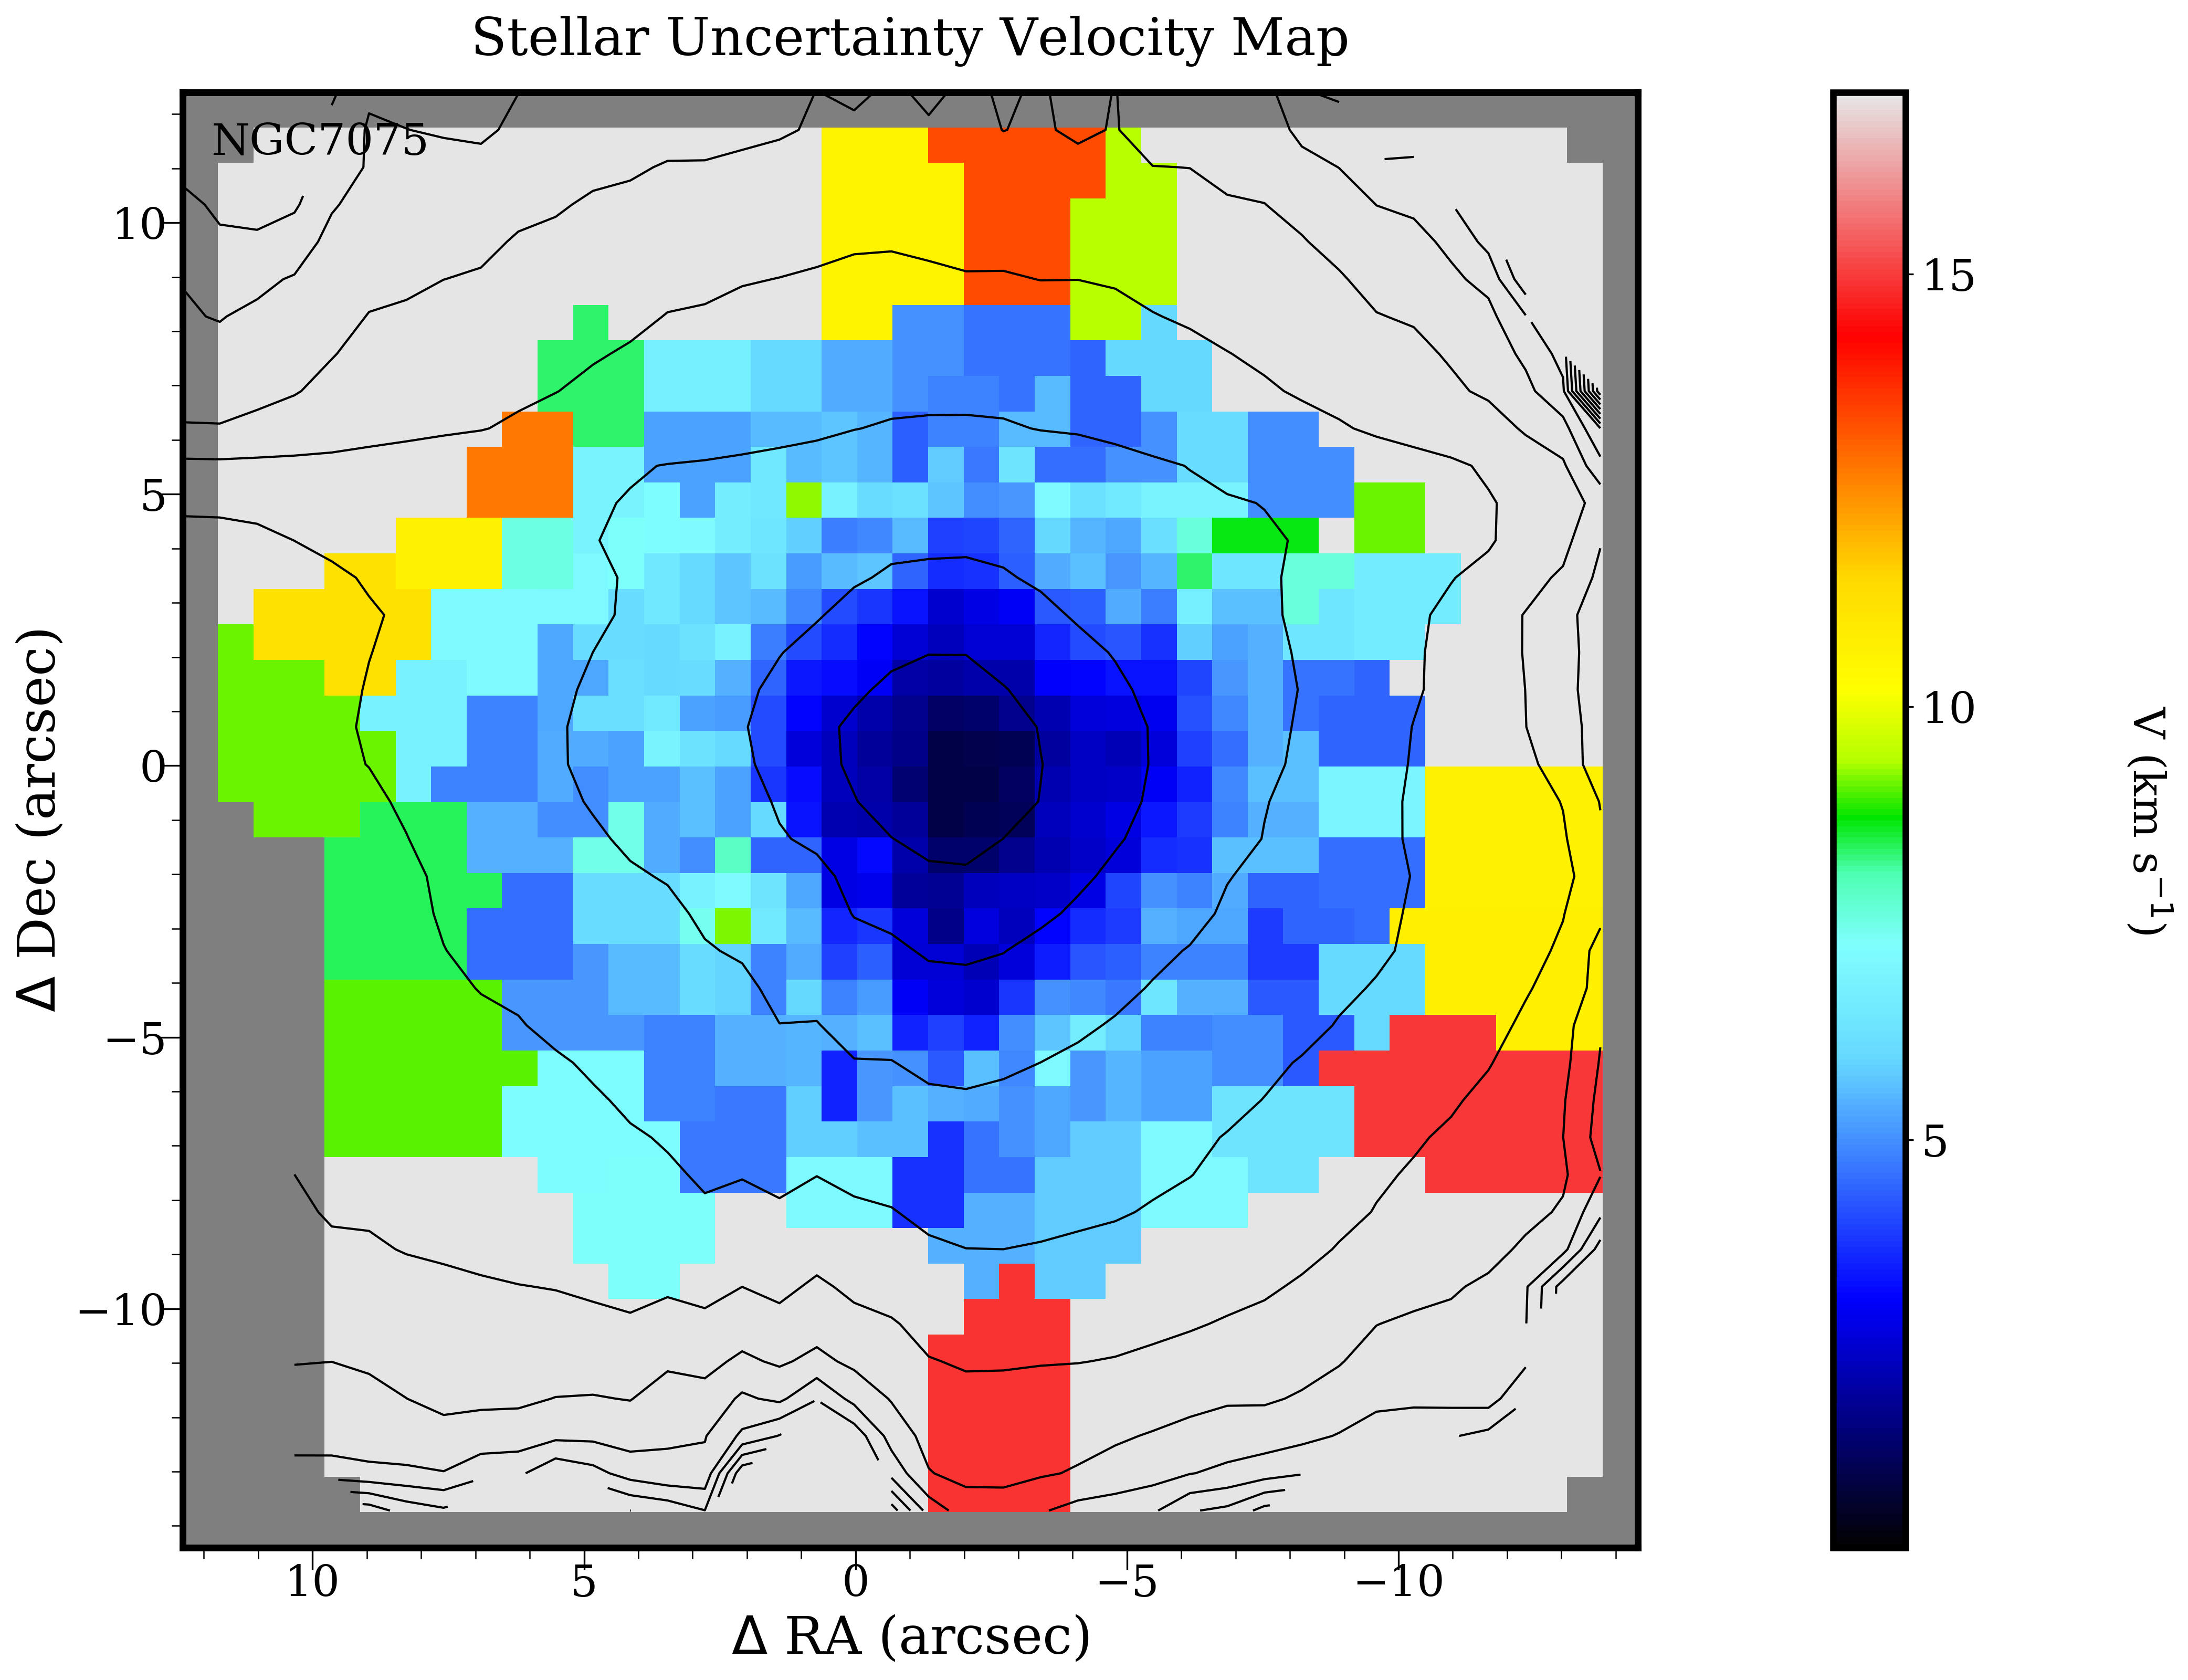
\includegraphics[width=0.245\textwidth]{Vmaps/ngc7075_stellar_vel_uncert.png}
      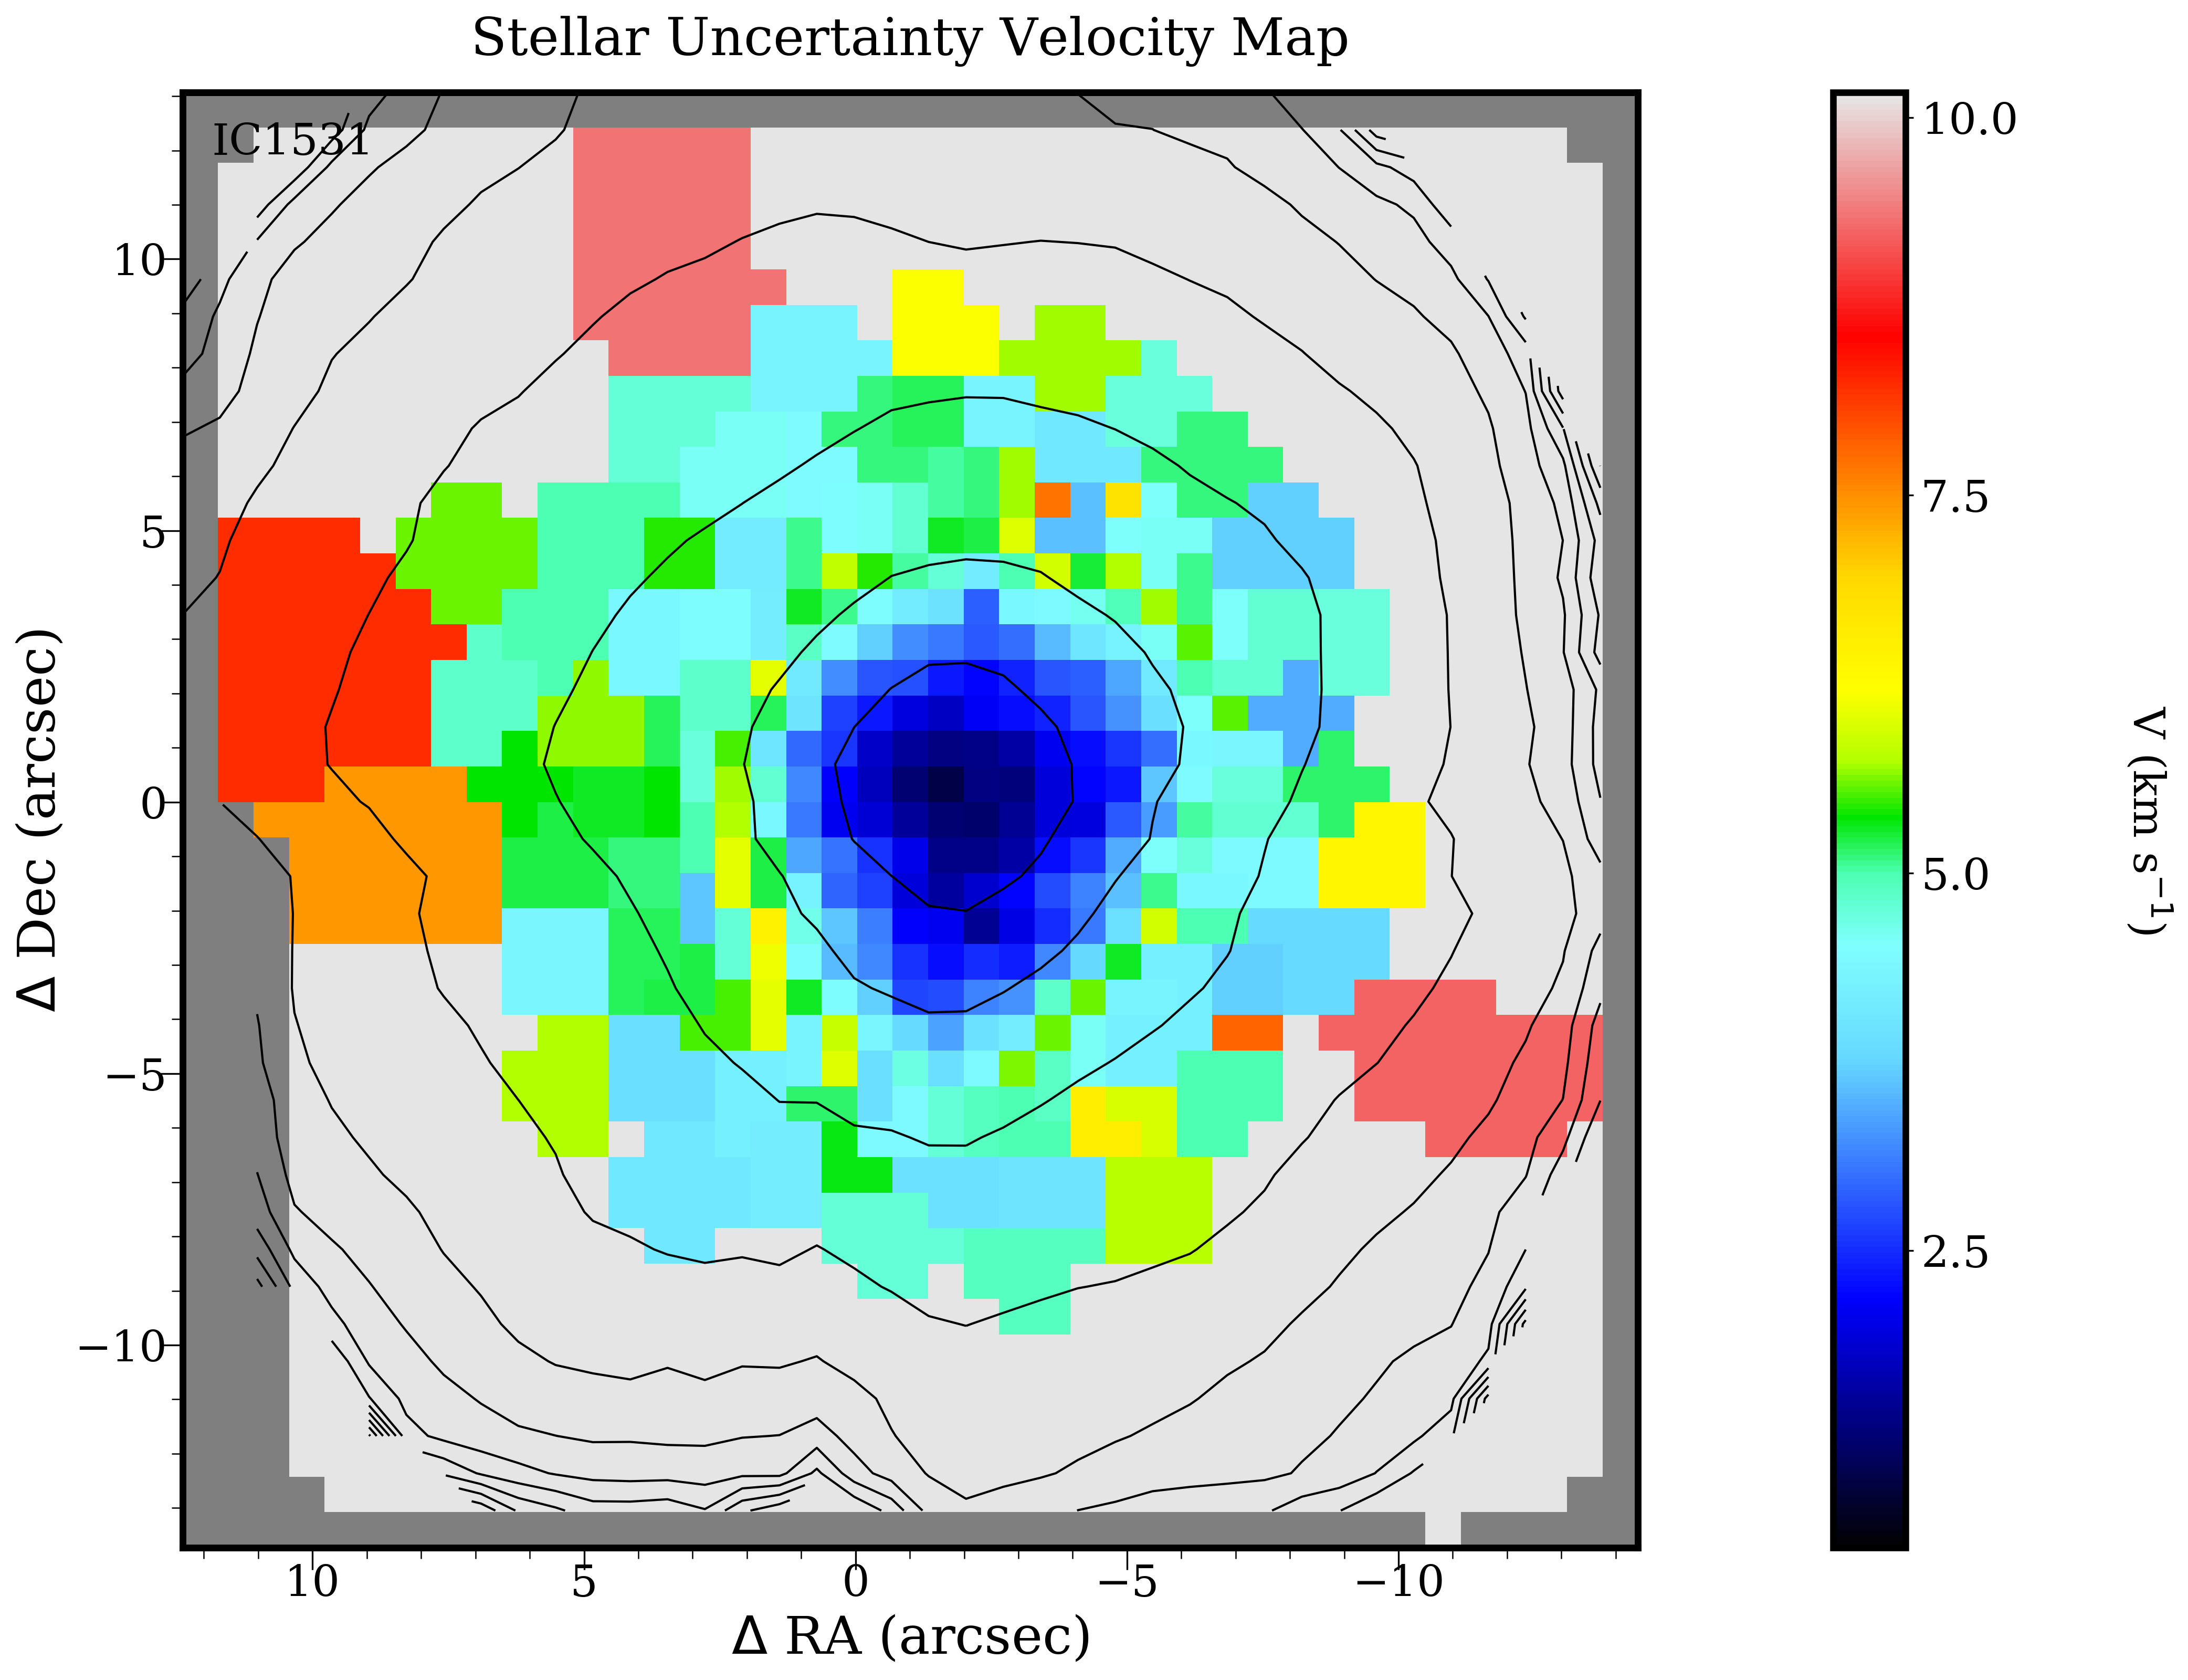
\includegraphics[width=0.245\textwidth]{Vmaps/ic1531_stellar_vel_uncert.png}
      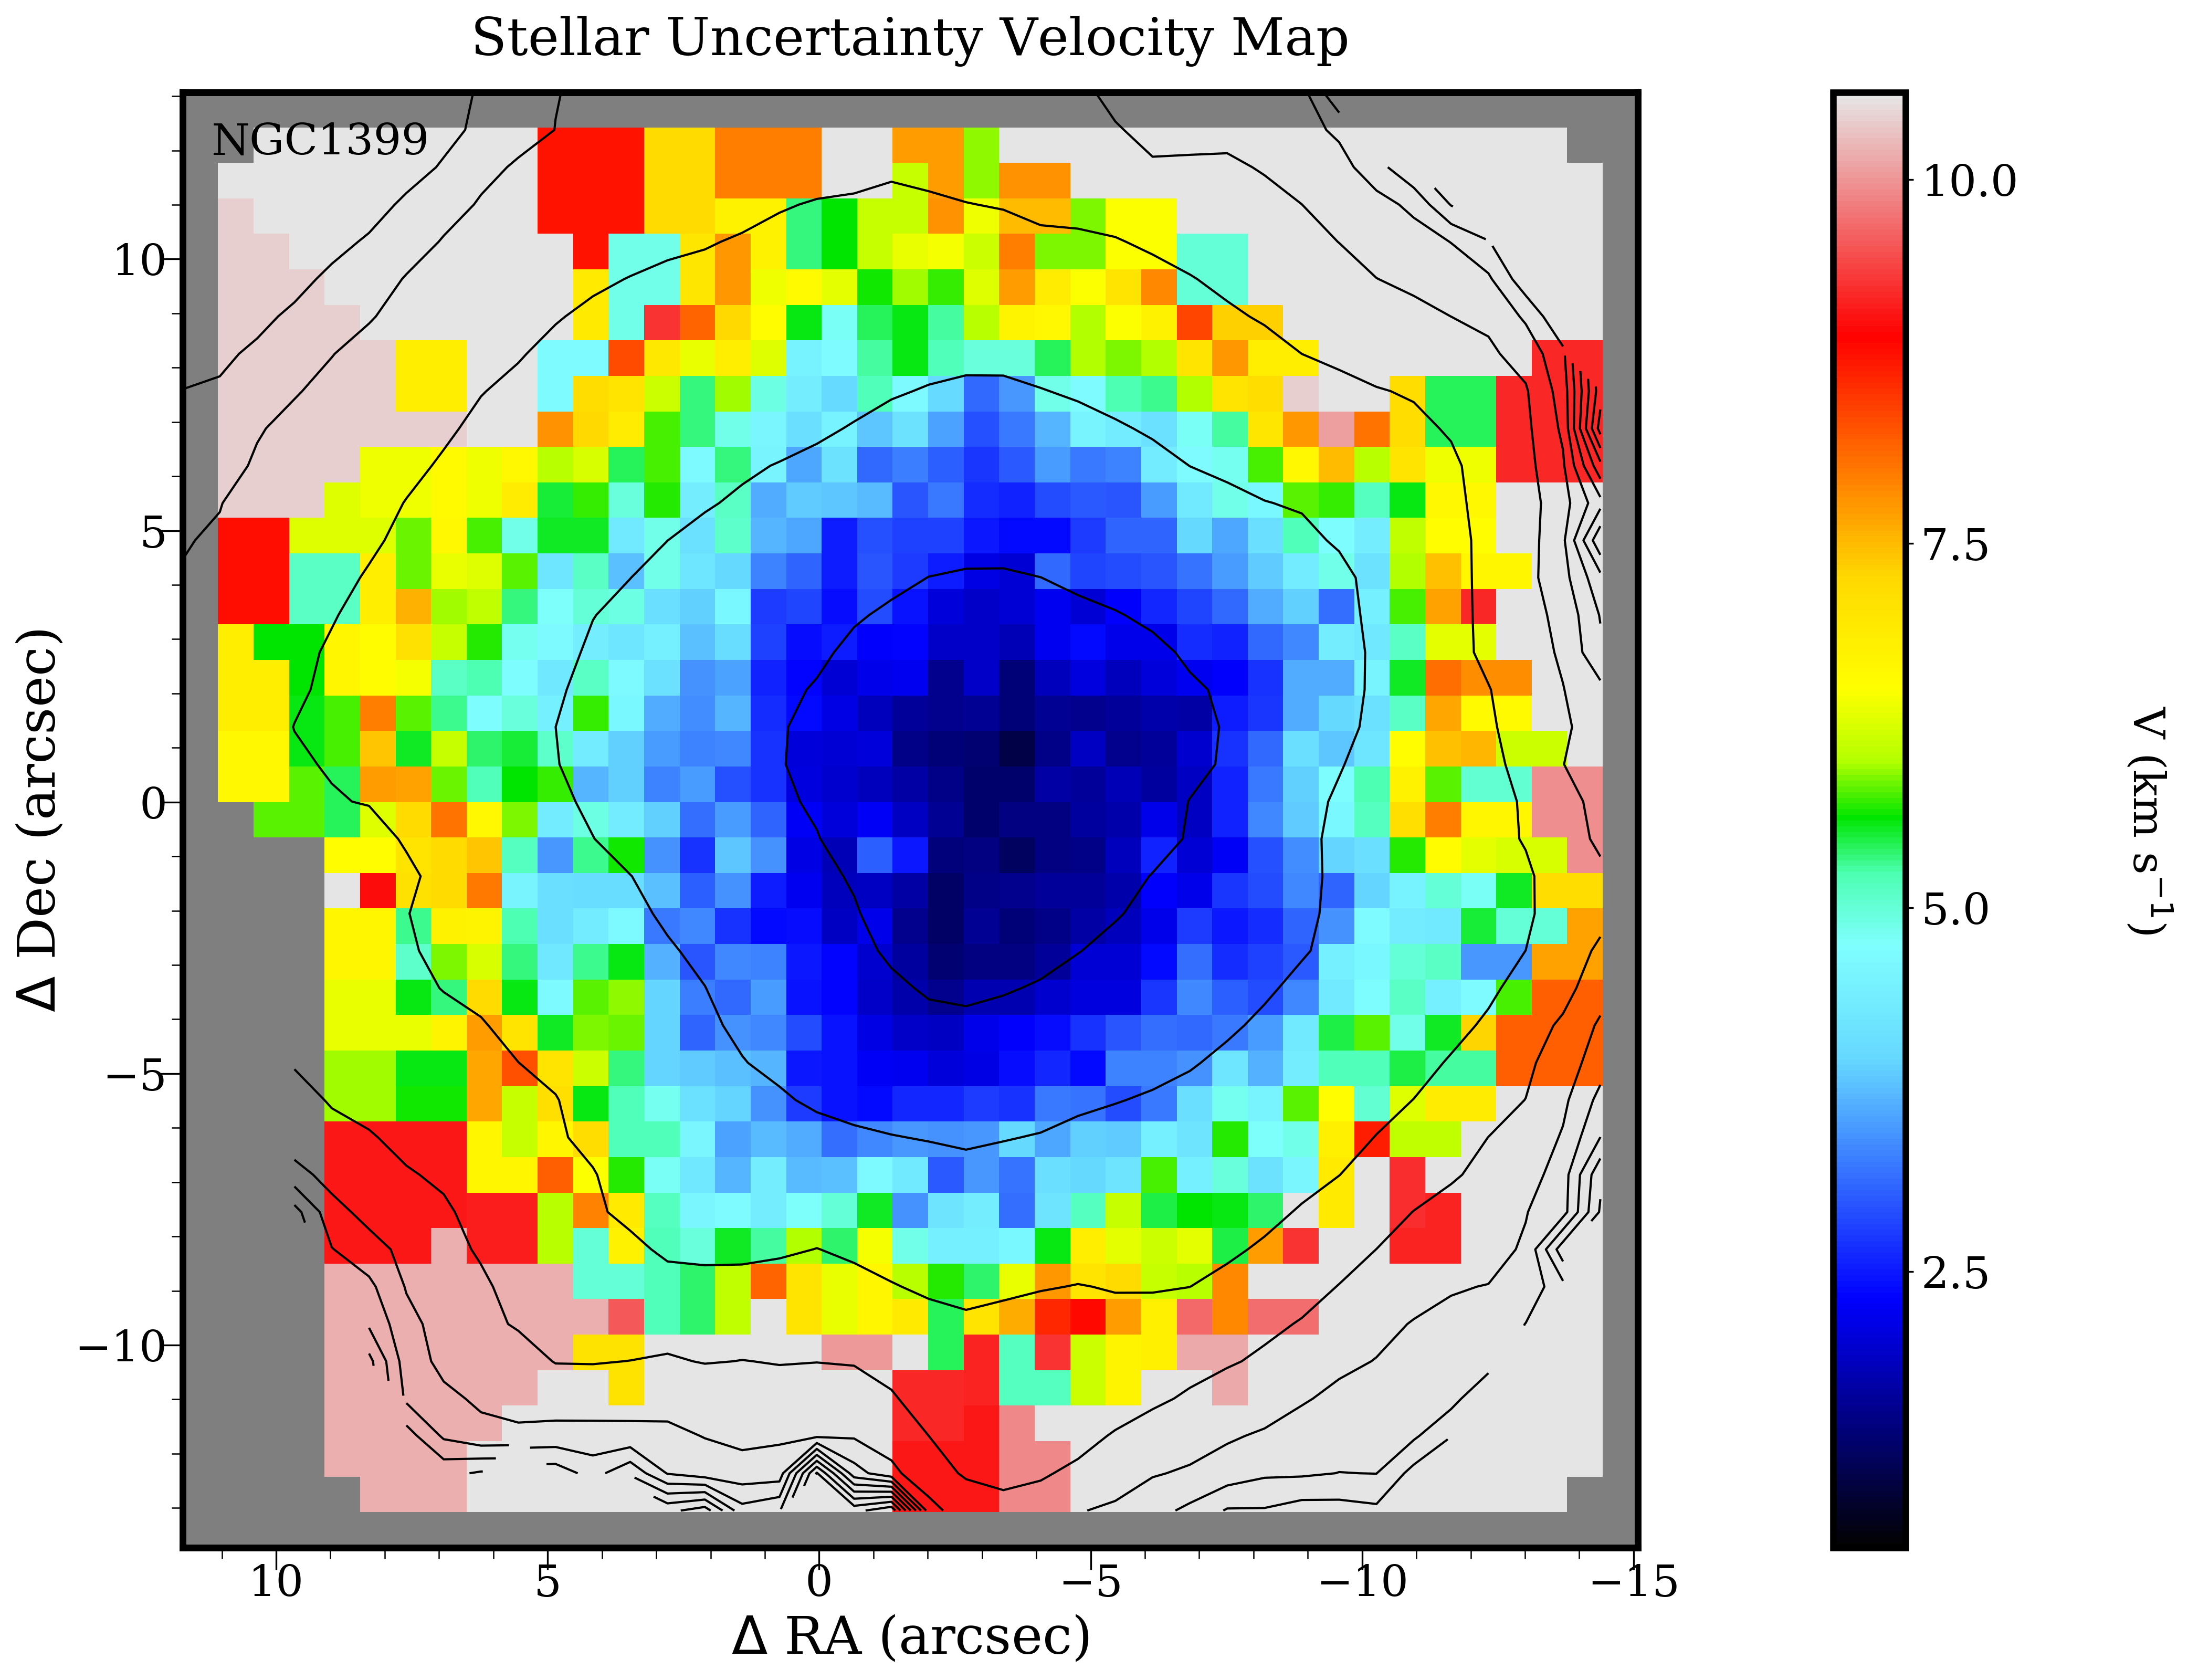
\includegraphics[width=0.245\textwidth]{Vmaps/ngc1399_stellar_vel_uncert.png}
      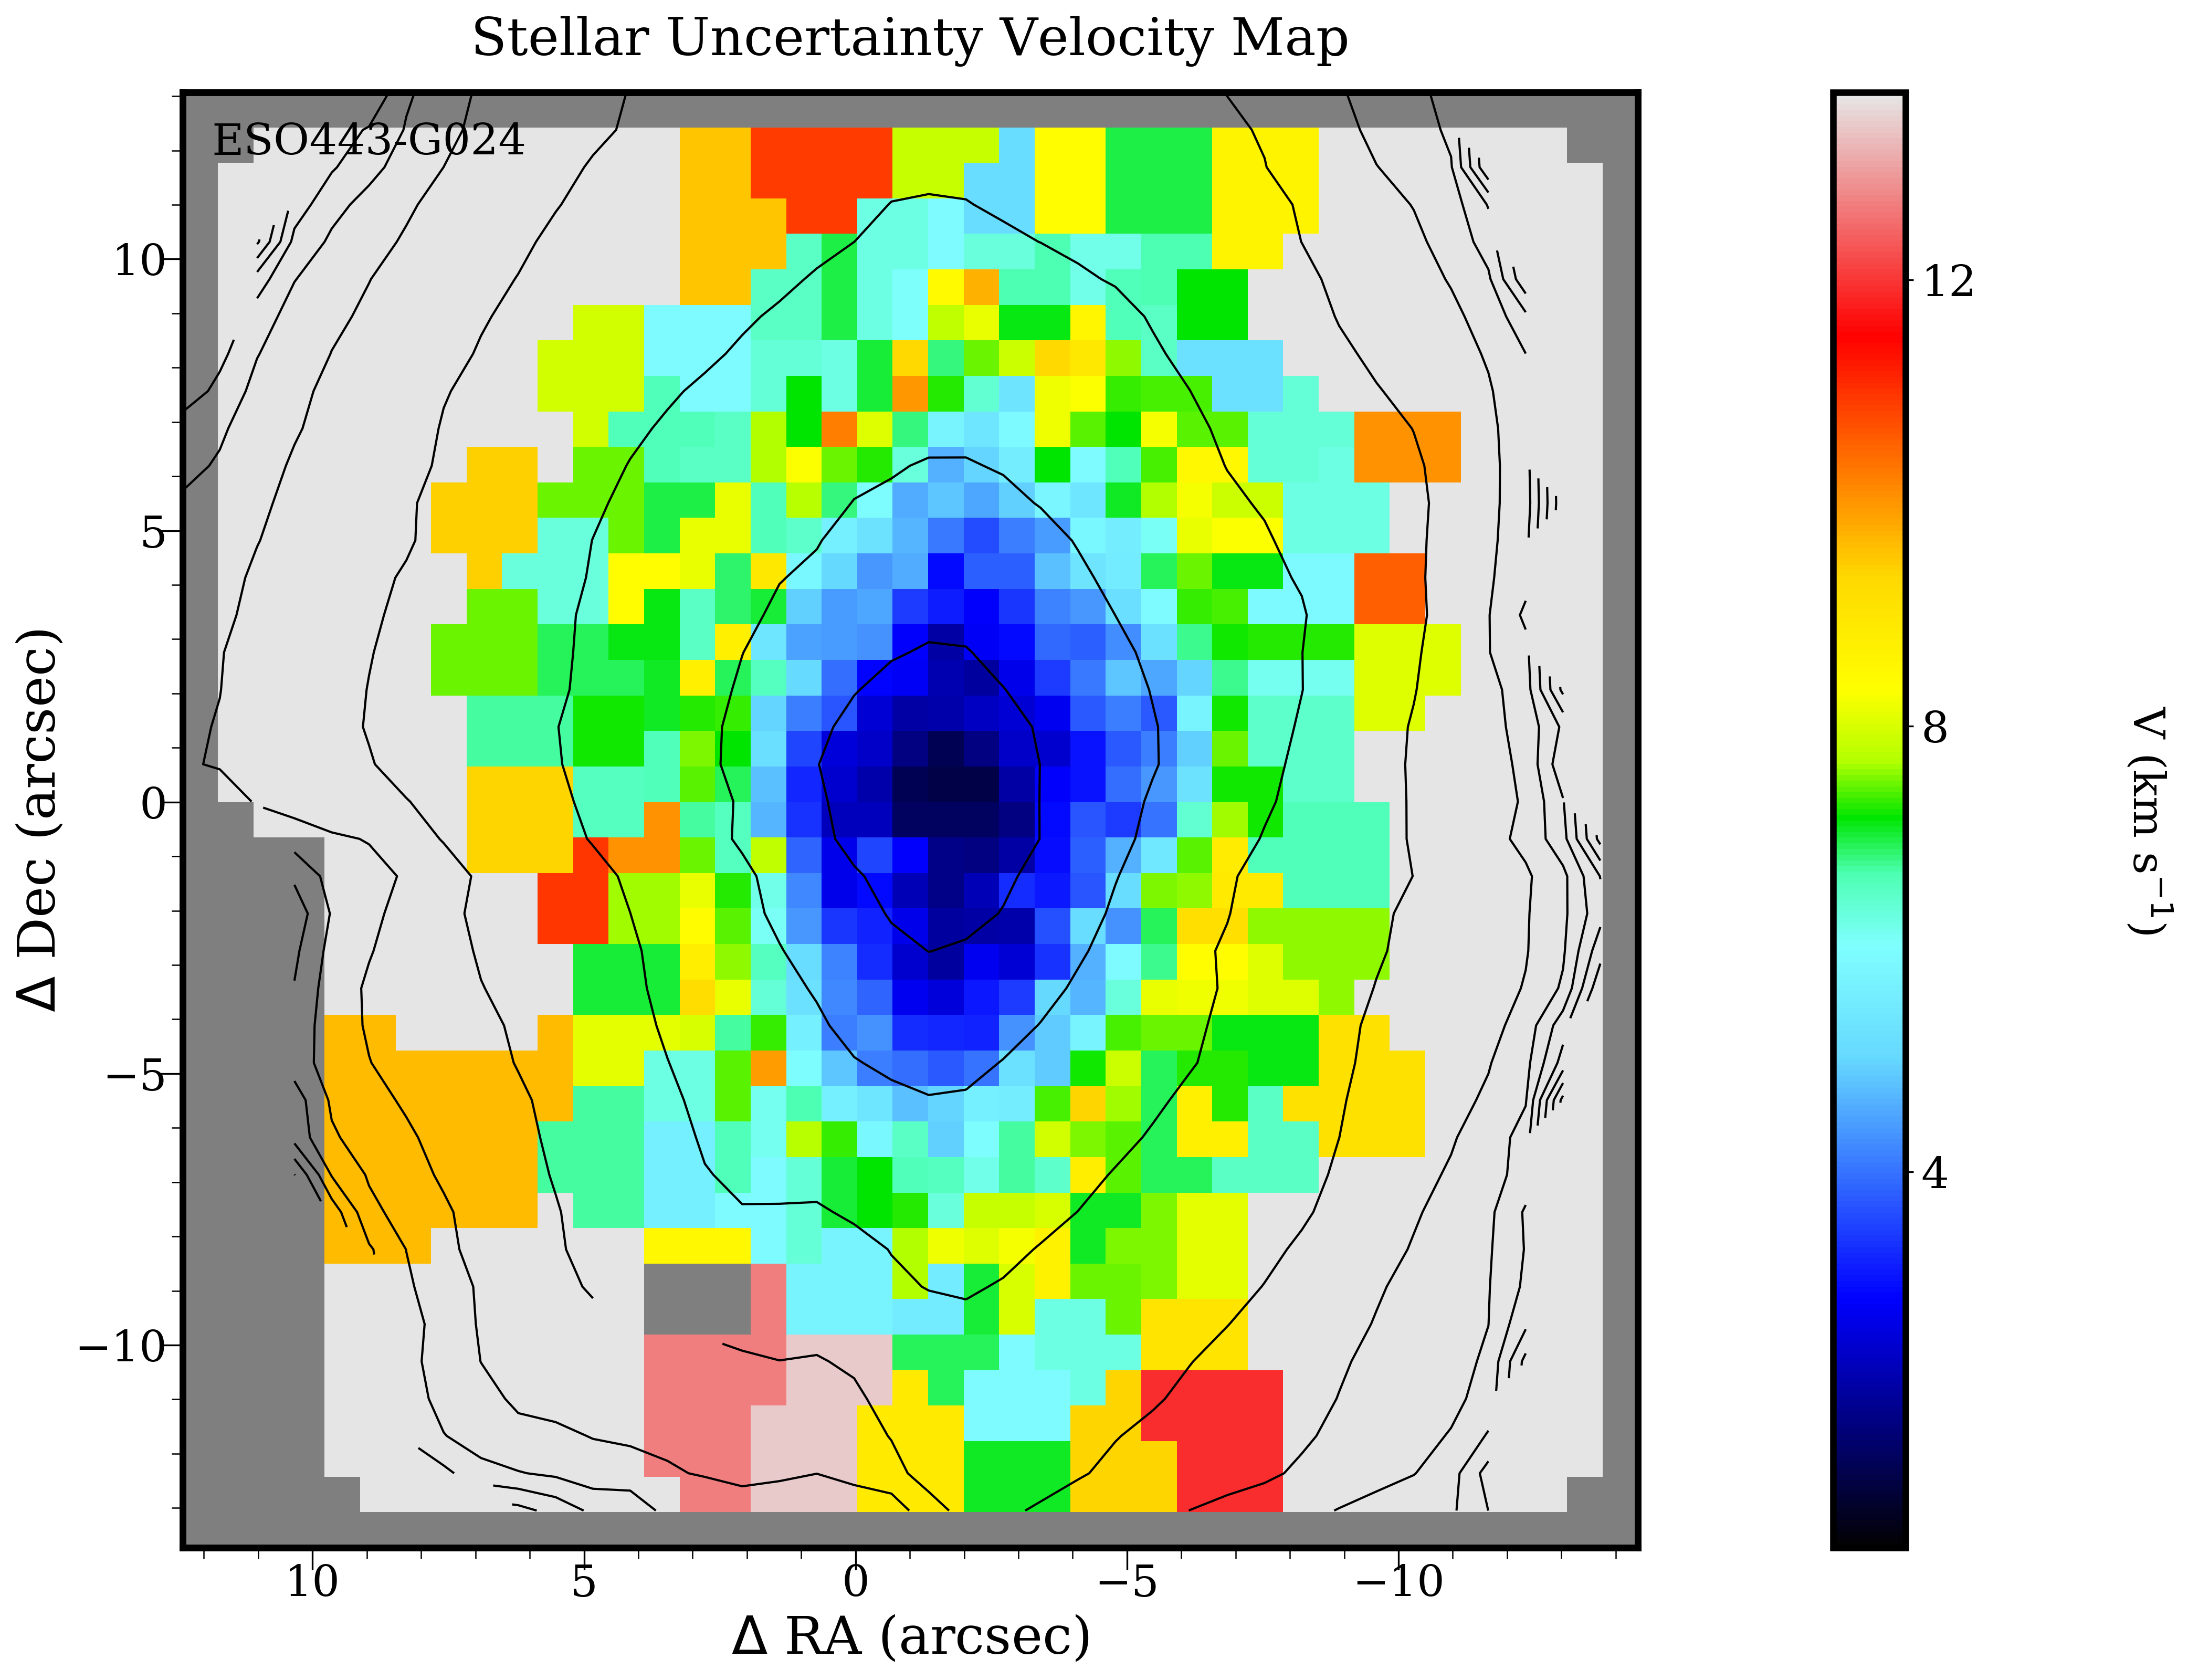
\includegraphics[width=0.245\textwidth]{Vmaps/eso443-g024_stellar_vel_uncert.png}
      \caption[VIMOS velocity uncertocity maps]{Uncertainties in the velocity for each galaxy in the VIMOS sample. Plots are ordered and contour colors are as in figure \ref{fig:Vstellar_img}}
      \label{fig:Vstellar_vel_uncert}
\end{figure*}

\begin{figure*}
      \centering
      \includegraphics[width=0.245\textwidth]{Vmaps/ngc0612_stellar_sigma.png}
      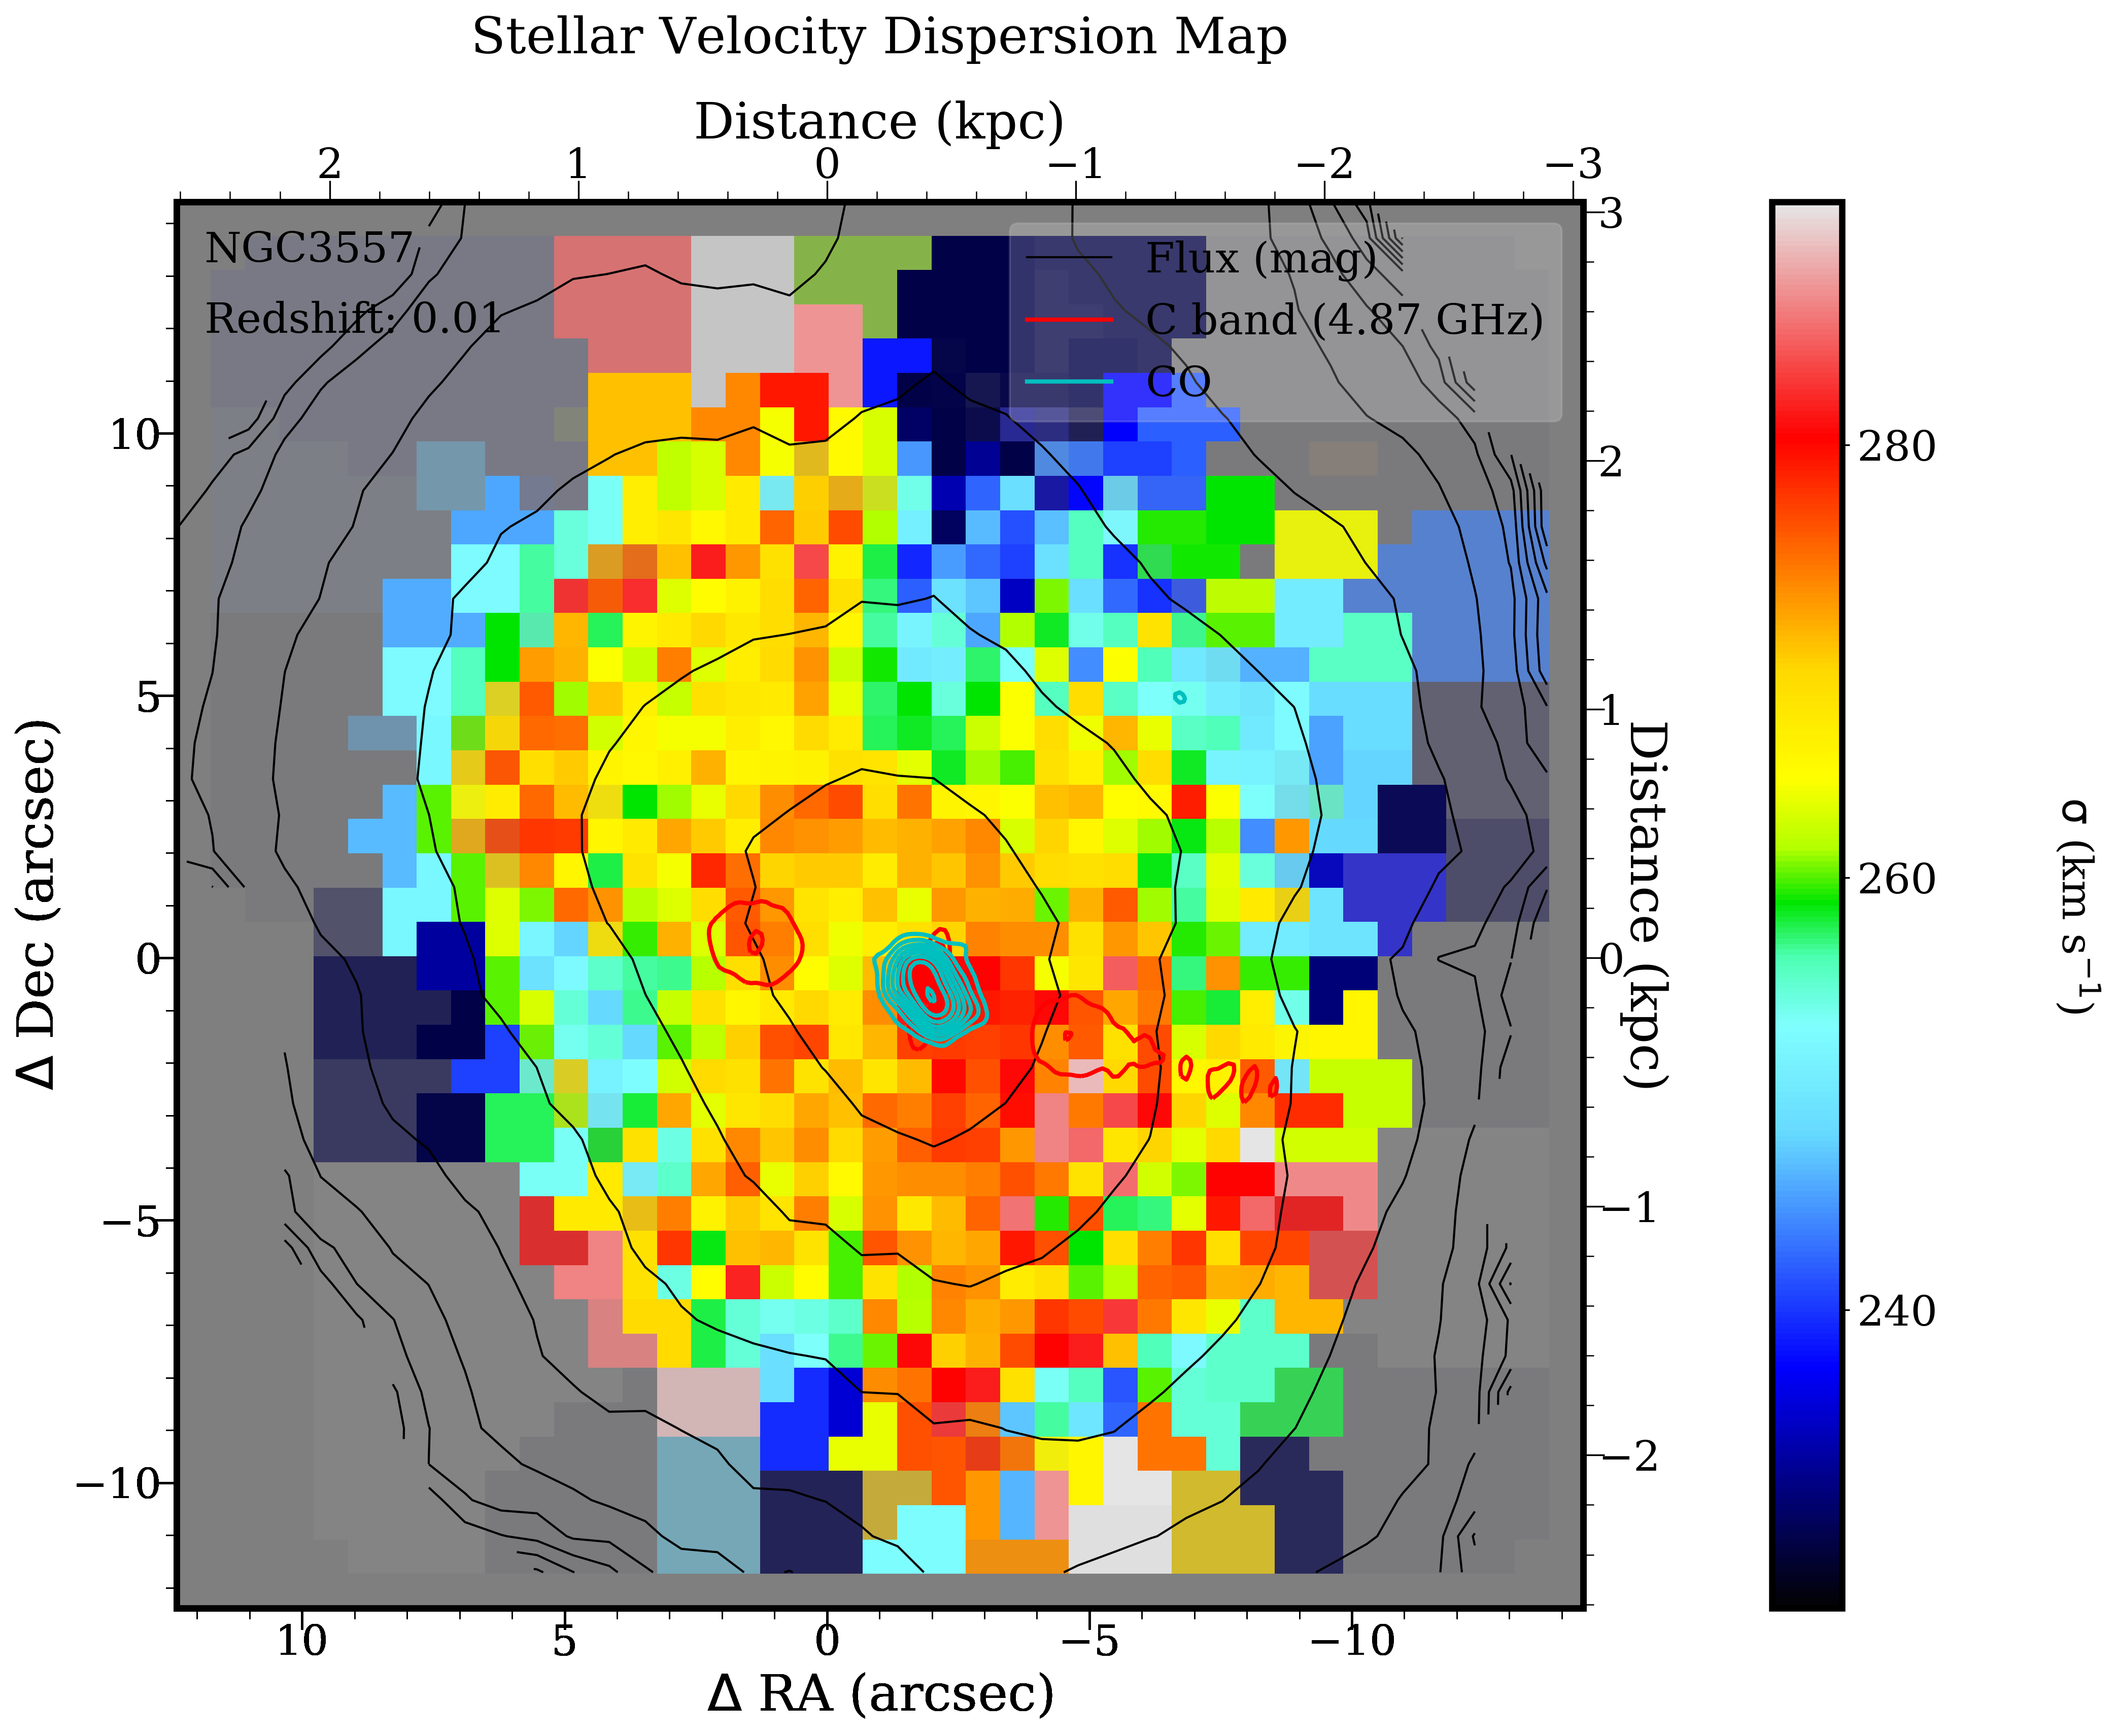
\includegraphics[width=0.245\textwidth]{Vmaps/ngc3557_stellar_sigma.png}
      \includegraphics[width=0.245\textwidth]{Vmaps/ngc3100_stellar_sigma.png}
      \includegraphics[width=0.245\textwidth]{Vmaps/ic1459_stellar_sigma.png}
      \includegraphics[width=0.245\textwidth]{Vmaps/pks0718-34_stellar_sigma.png}
      \includegraphics[width=0.245\textwidth]{Vmaps/ic4296_stellar_sigma.png}
      \includegraphics[width=0.245\textwidth]{Vmaps/ngc7075_stellar_sigma.png}
      \includegraphics[width=0.245\textwidth]{Vmaps/ic1531_stellar_sigma.png}
      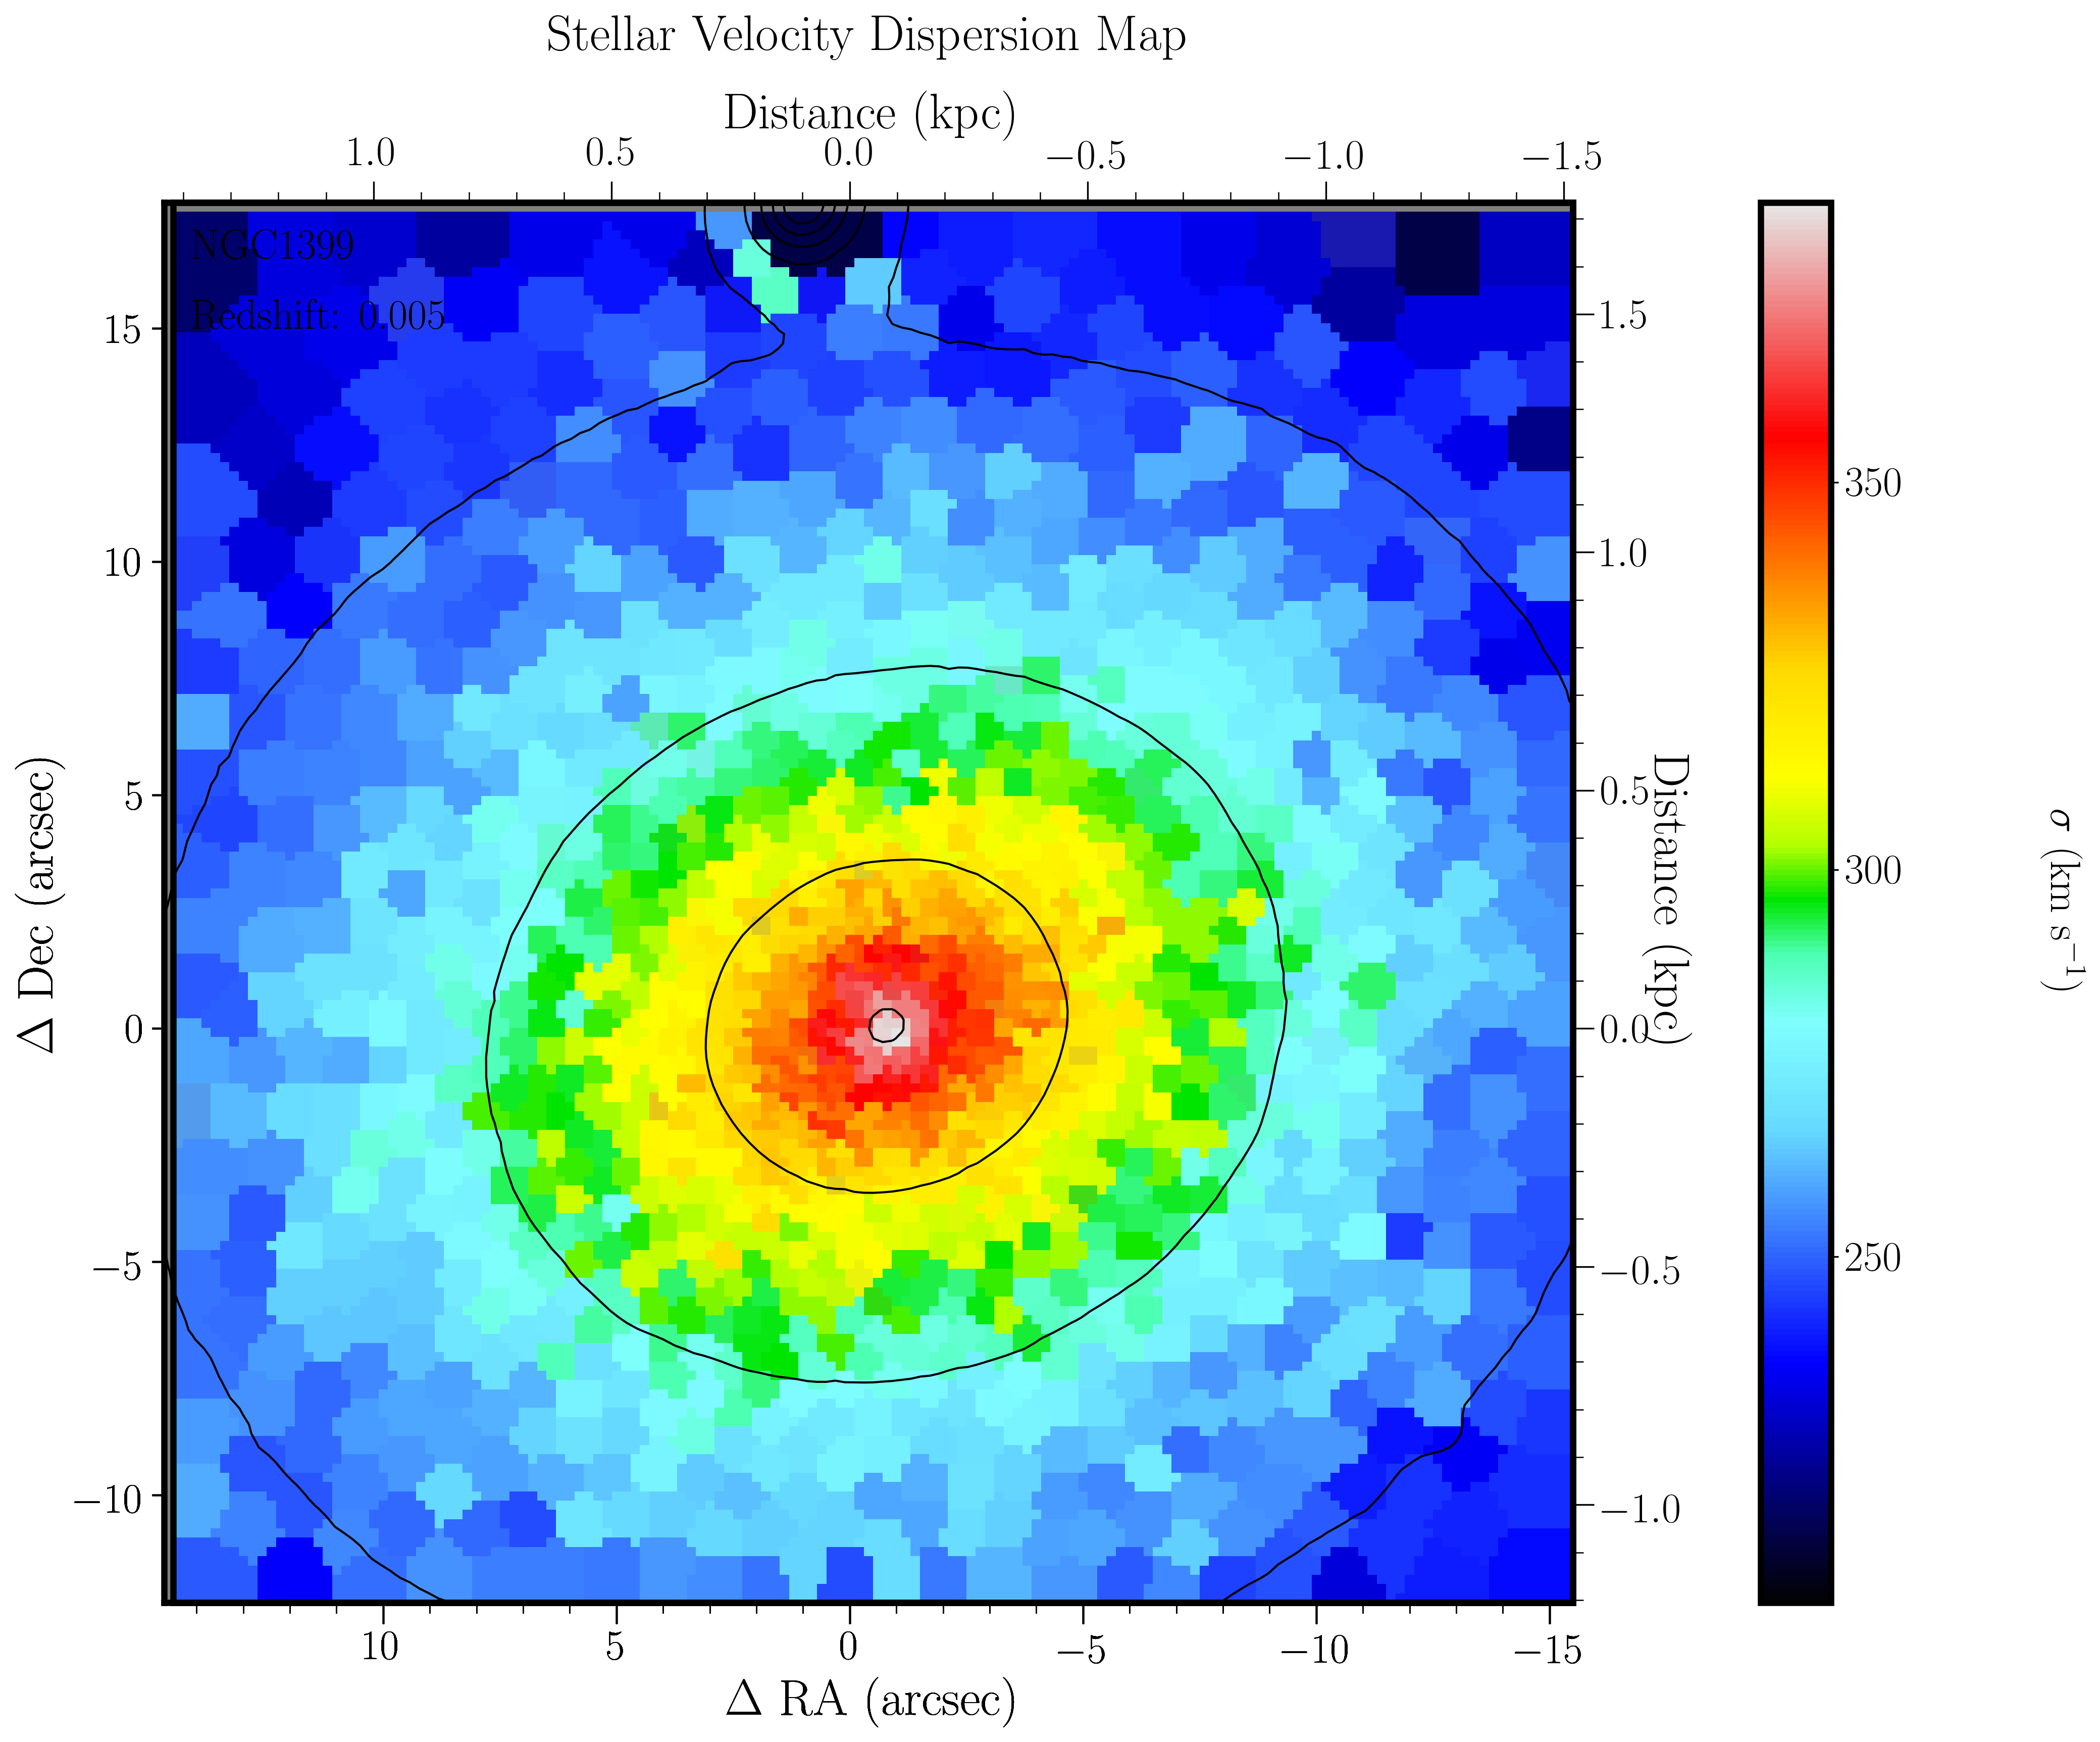
\includegraphics[width=0.245\textwidth]{Vmaps/ngc1399_stellar_sigma.png}
      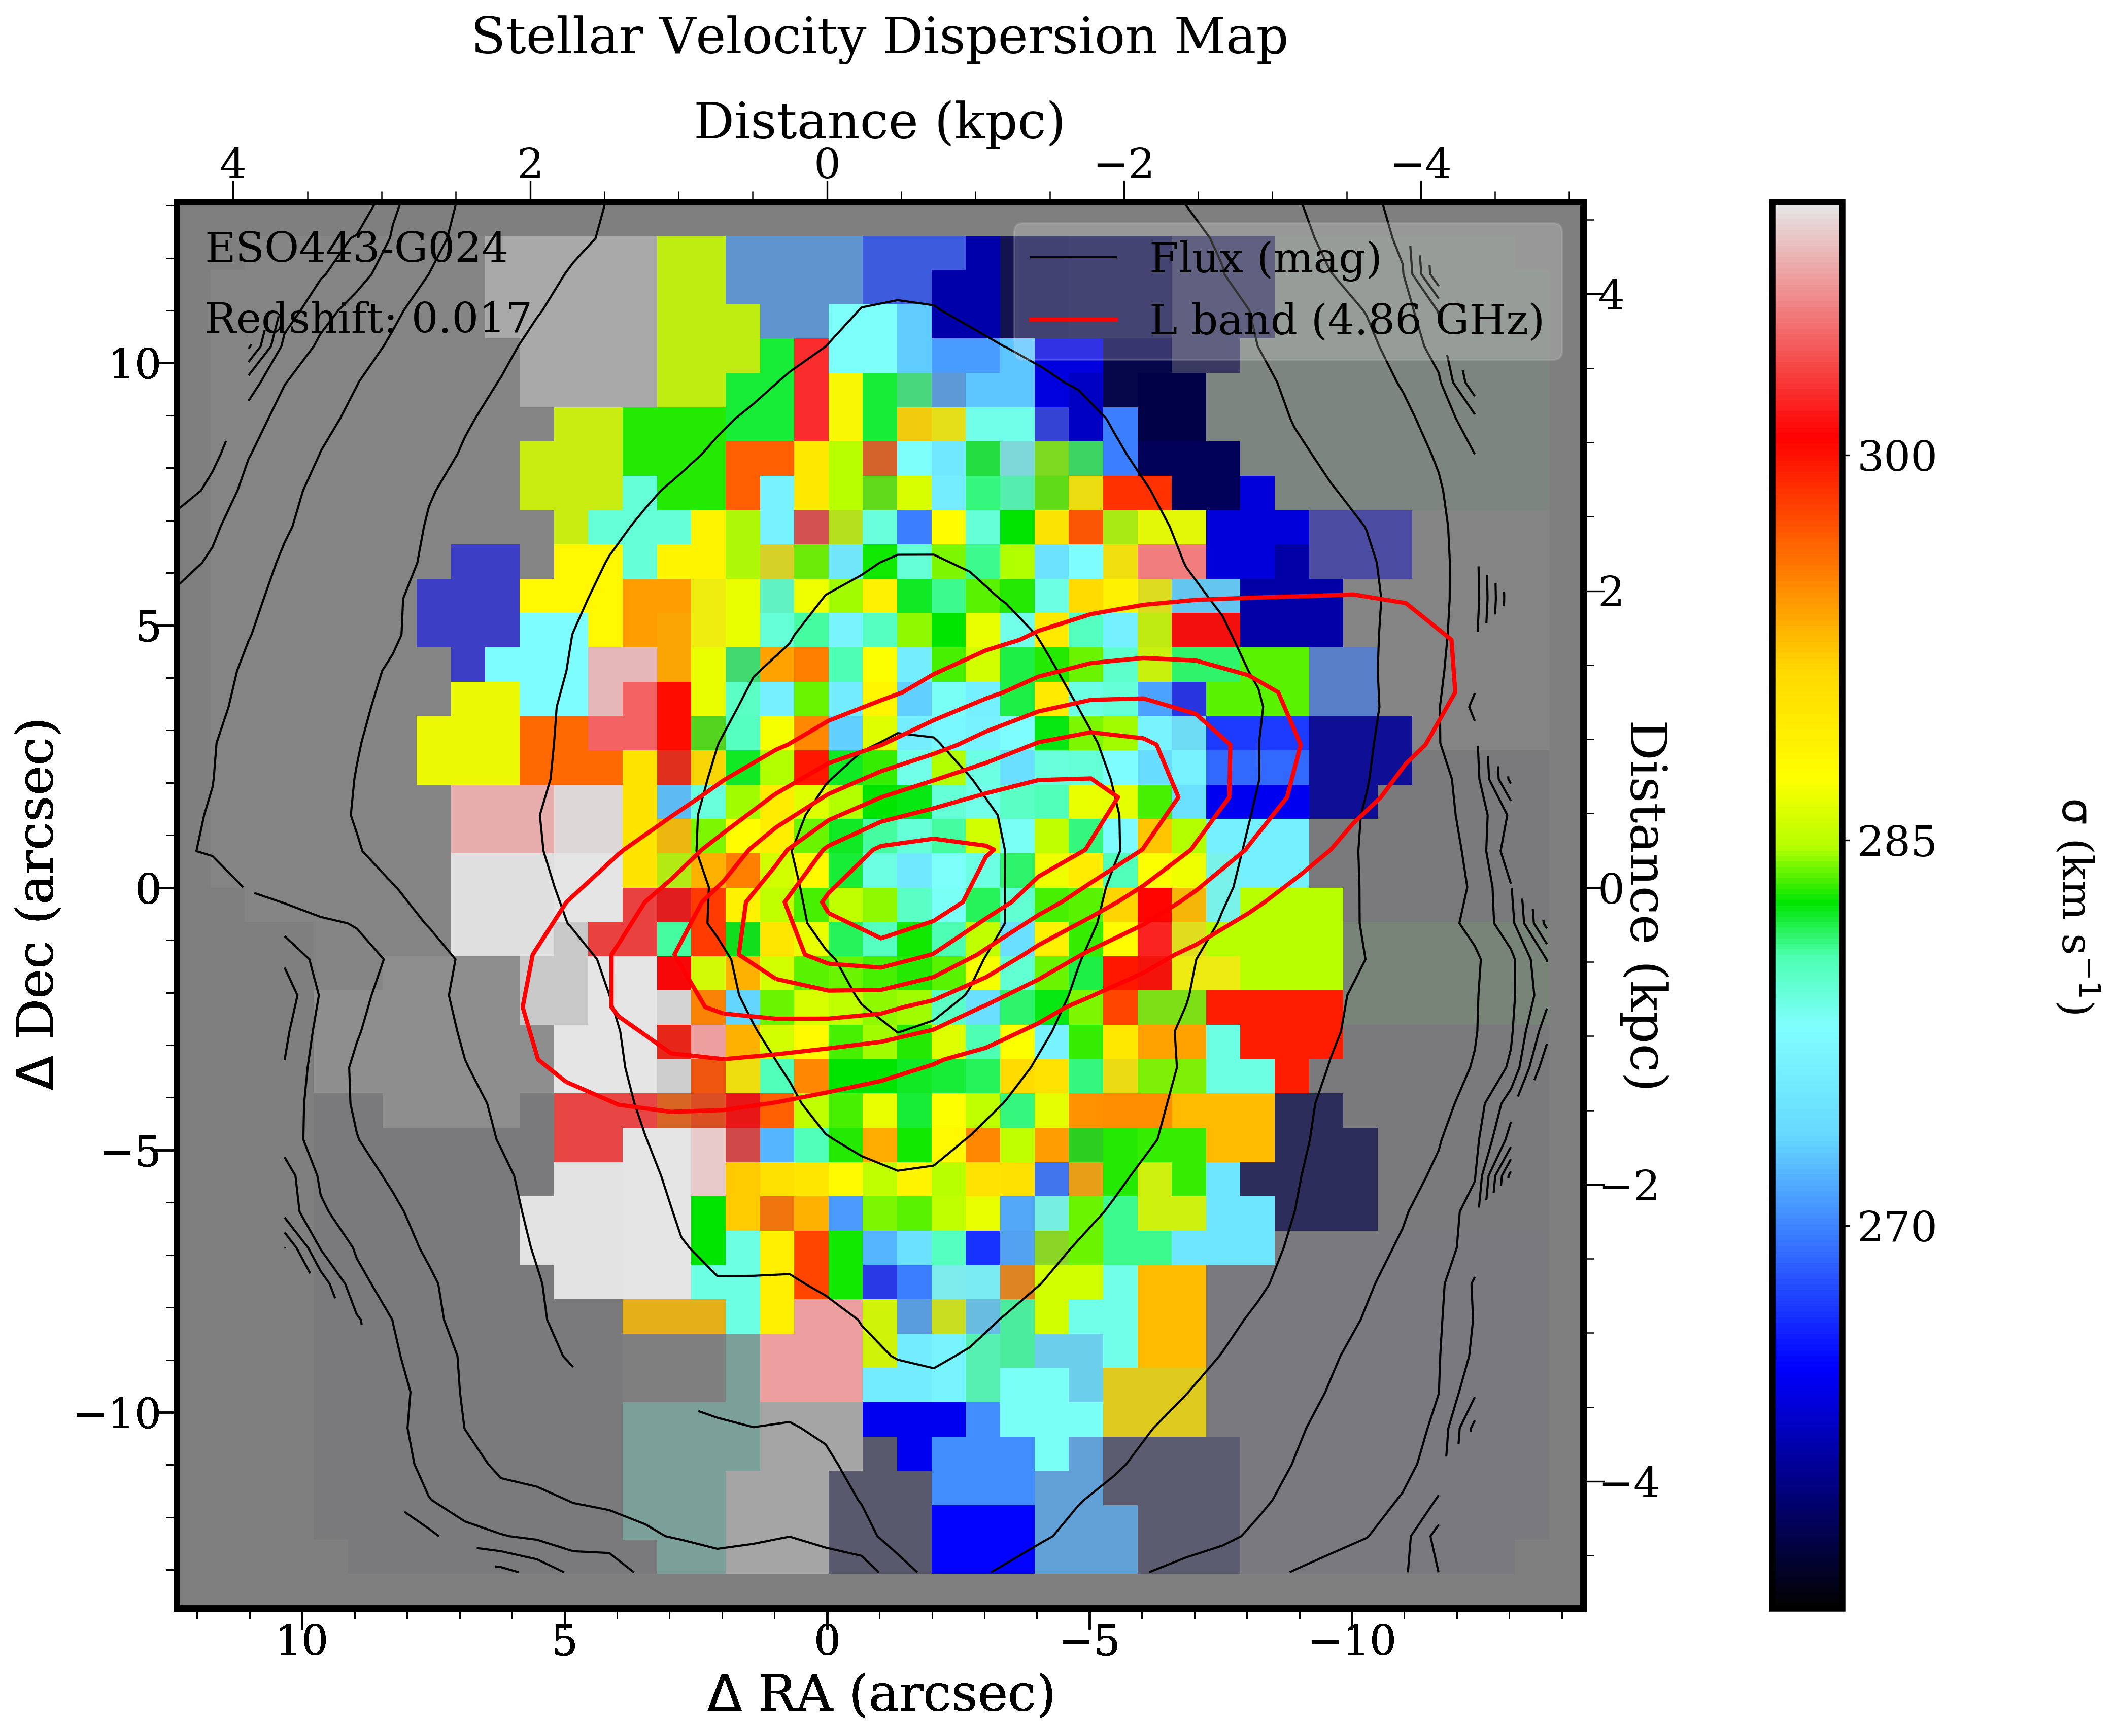
\includegraphics[width=0.245\textwidth]{Vmaps/eso443-g024_stellar_sigma.png}
      \caption[VIMOS velocity dispersion]{Velocity dispersion for each galaxy in the VIMOS sample. Plots are ordered and contour colors are as in figure \ref{fig:Vstellar_img}}
      \label{fig:Vstellar_sigma}
\end{figure*}


\begin{figure*}
      \centering
      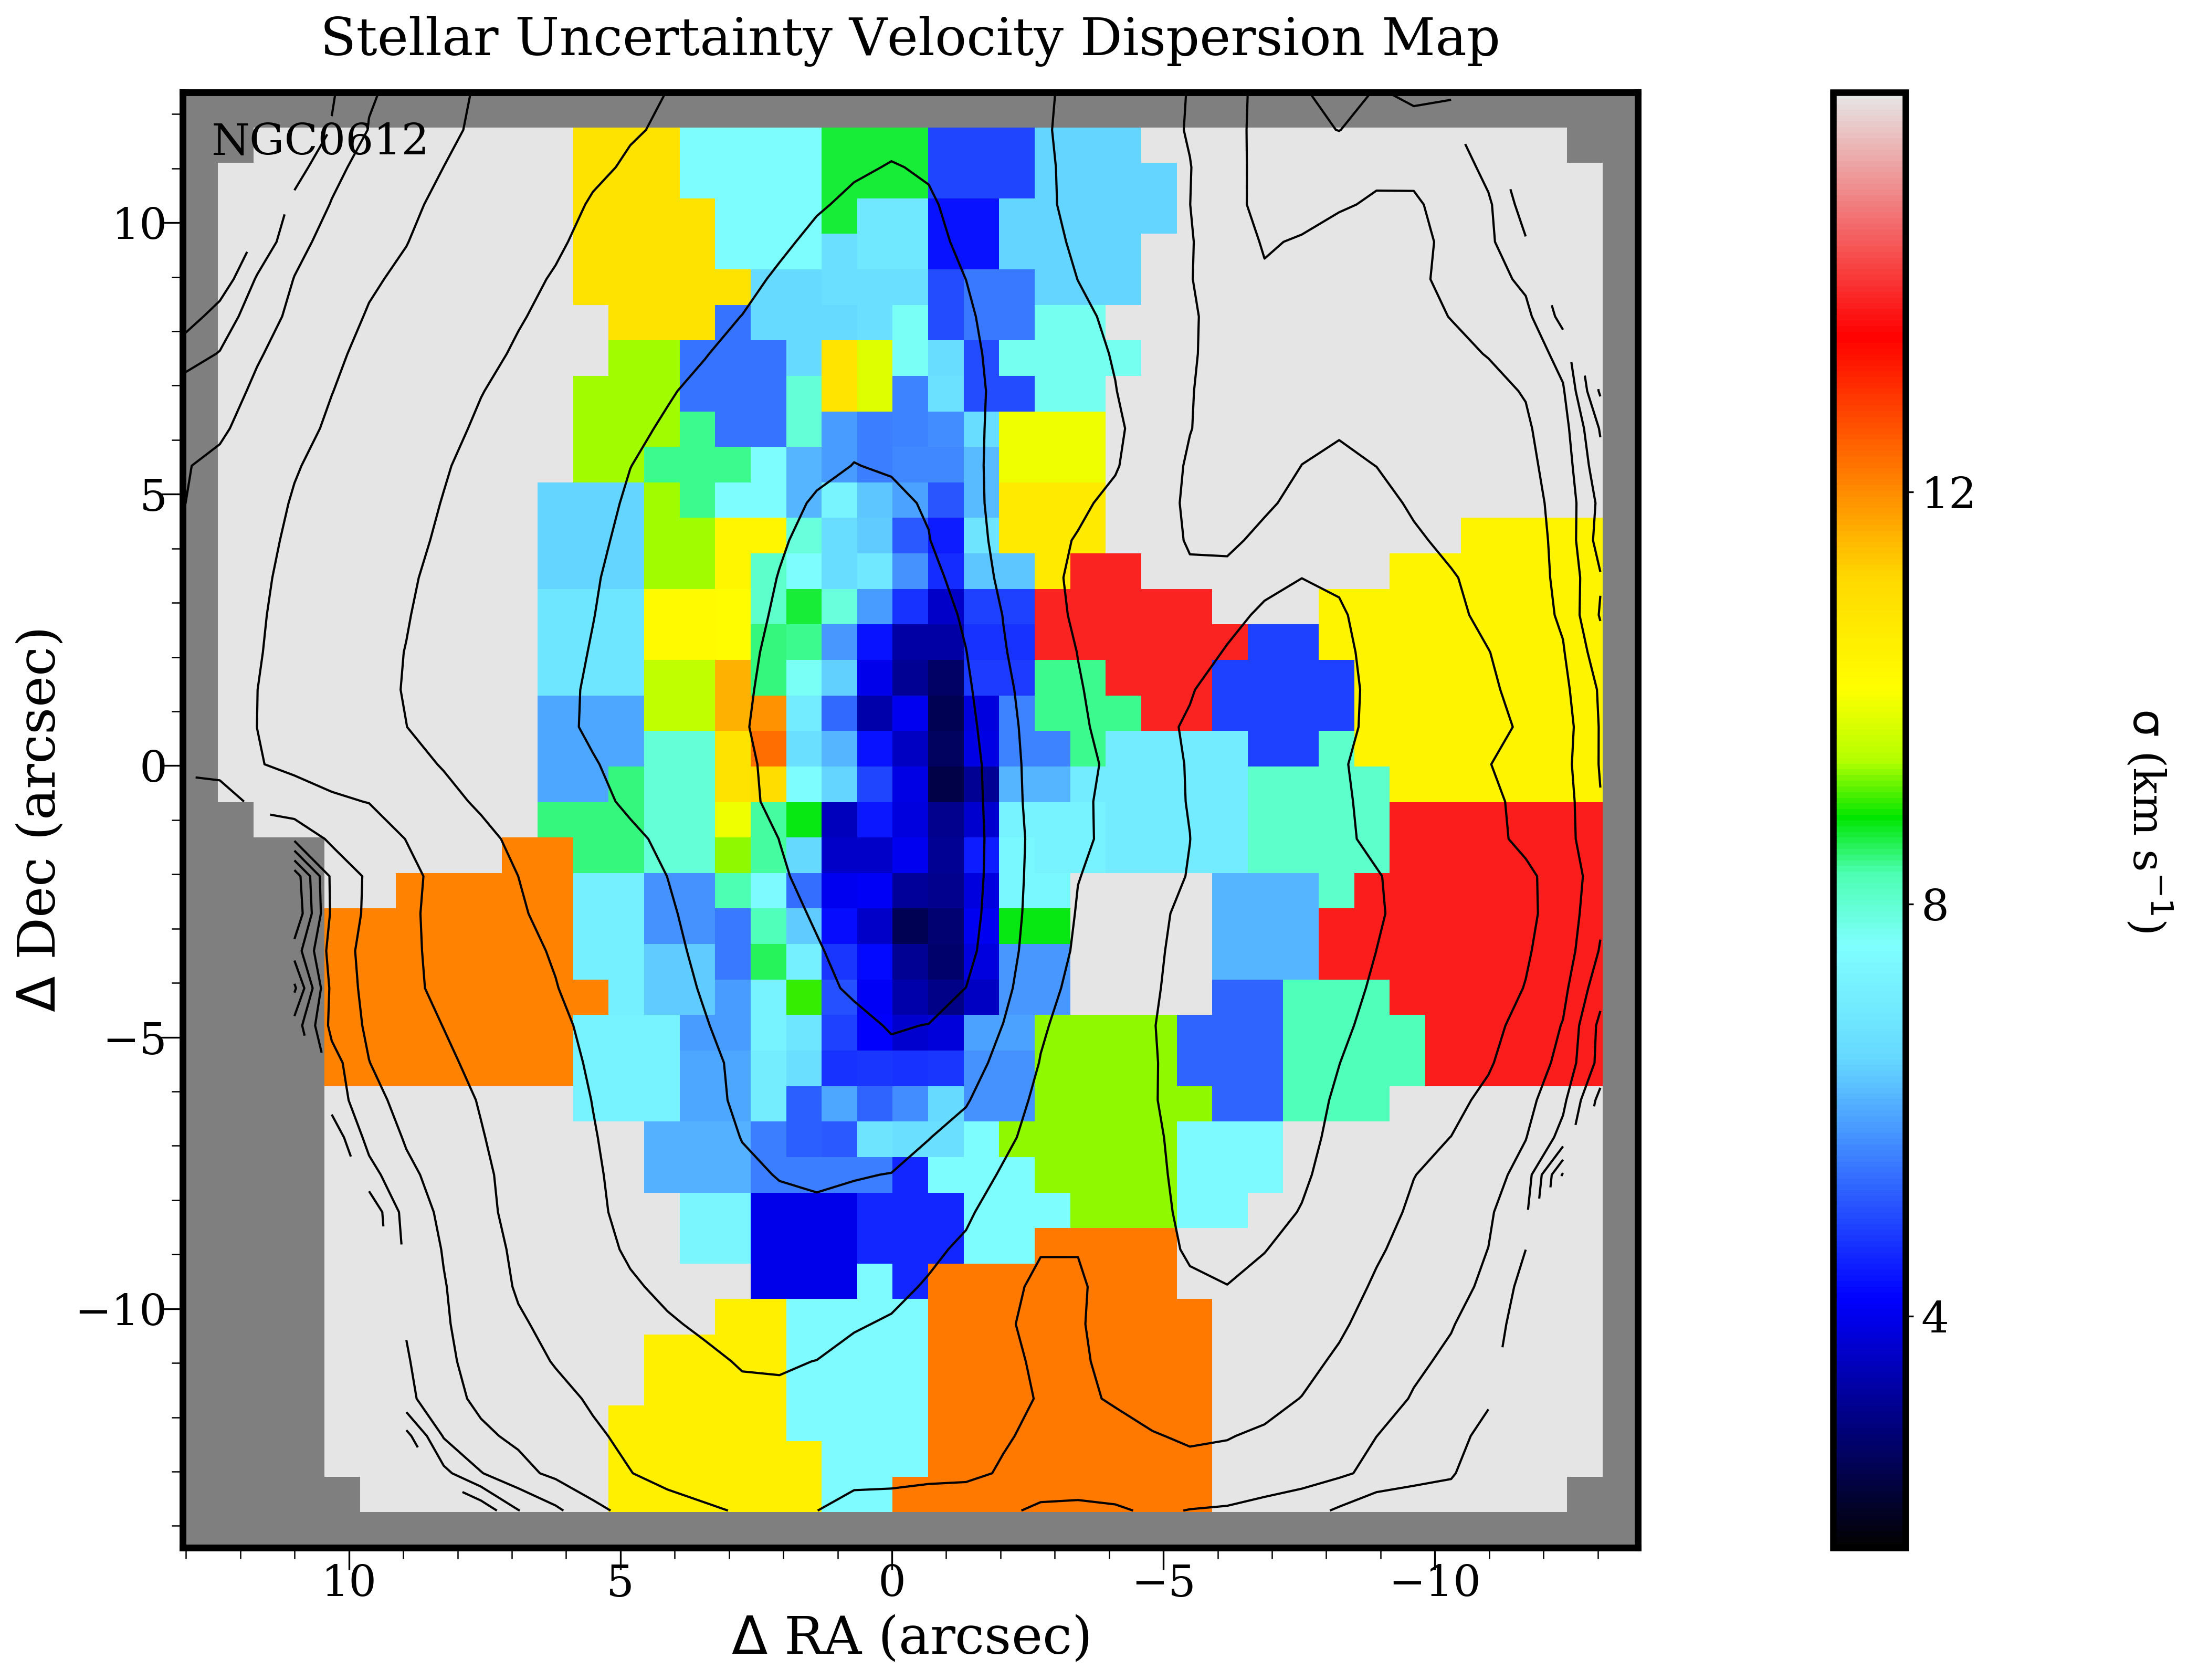
\includegraphics[width=0.245\textwidth]{Vmaps/ngc0612_stellar_sigma_uncert.png}
      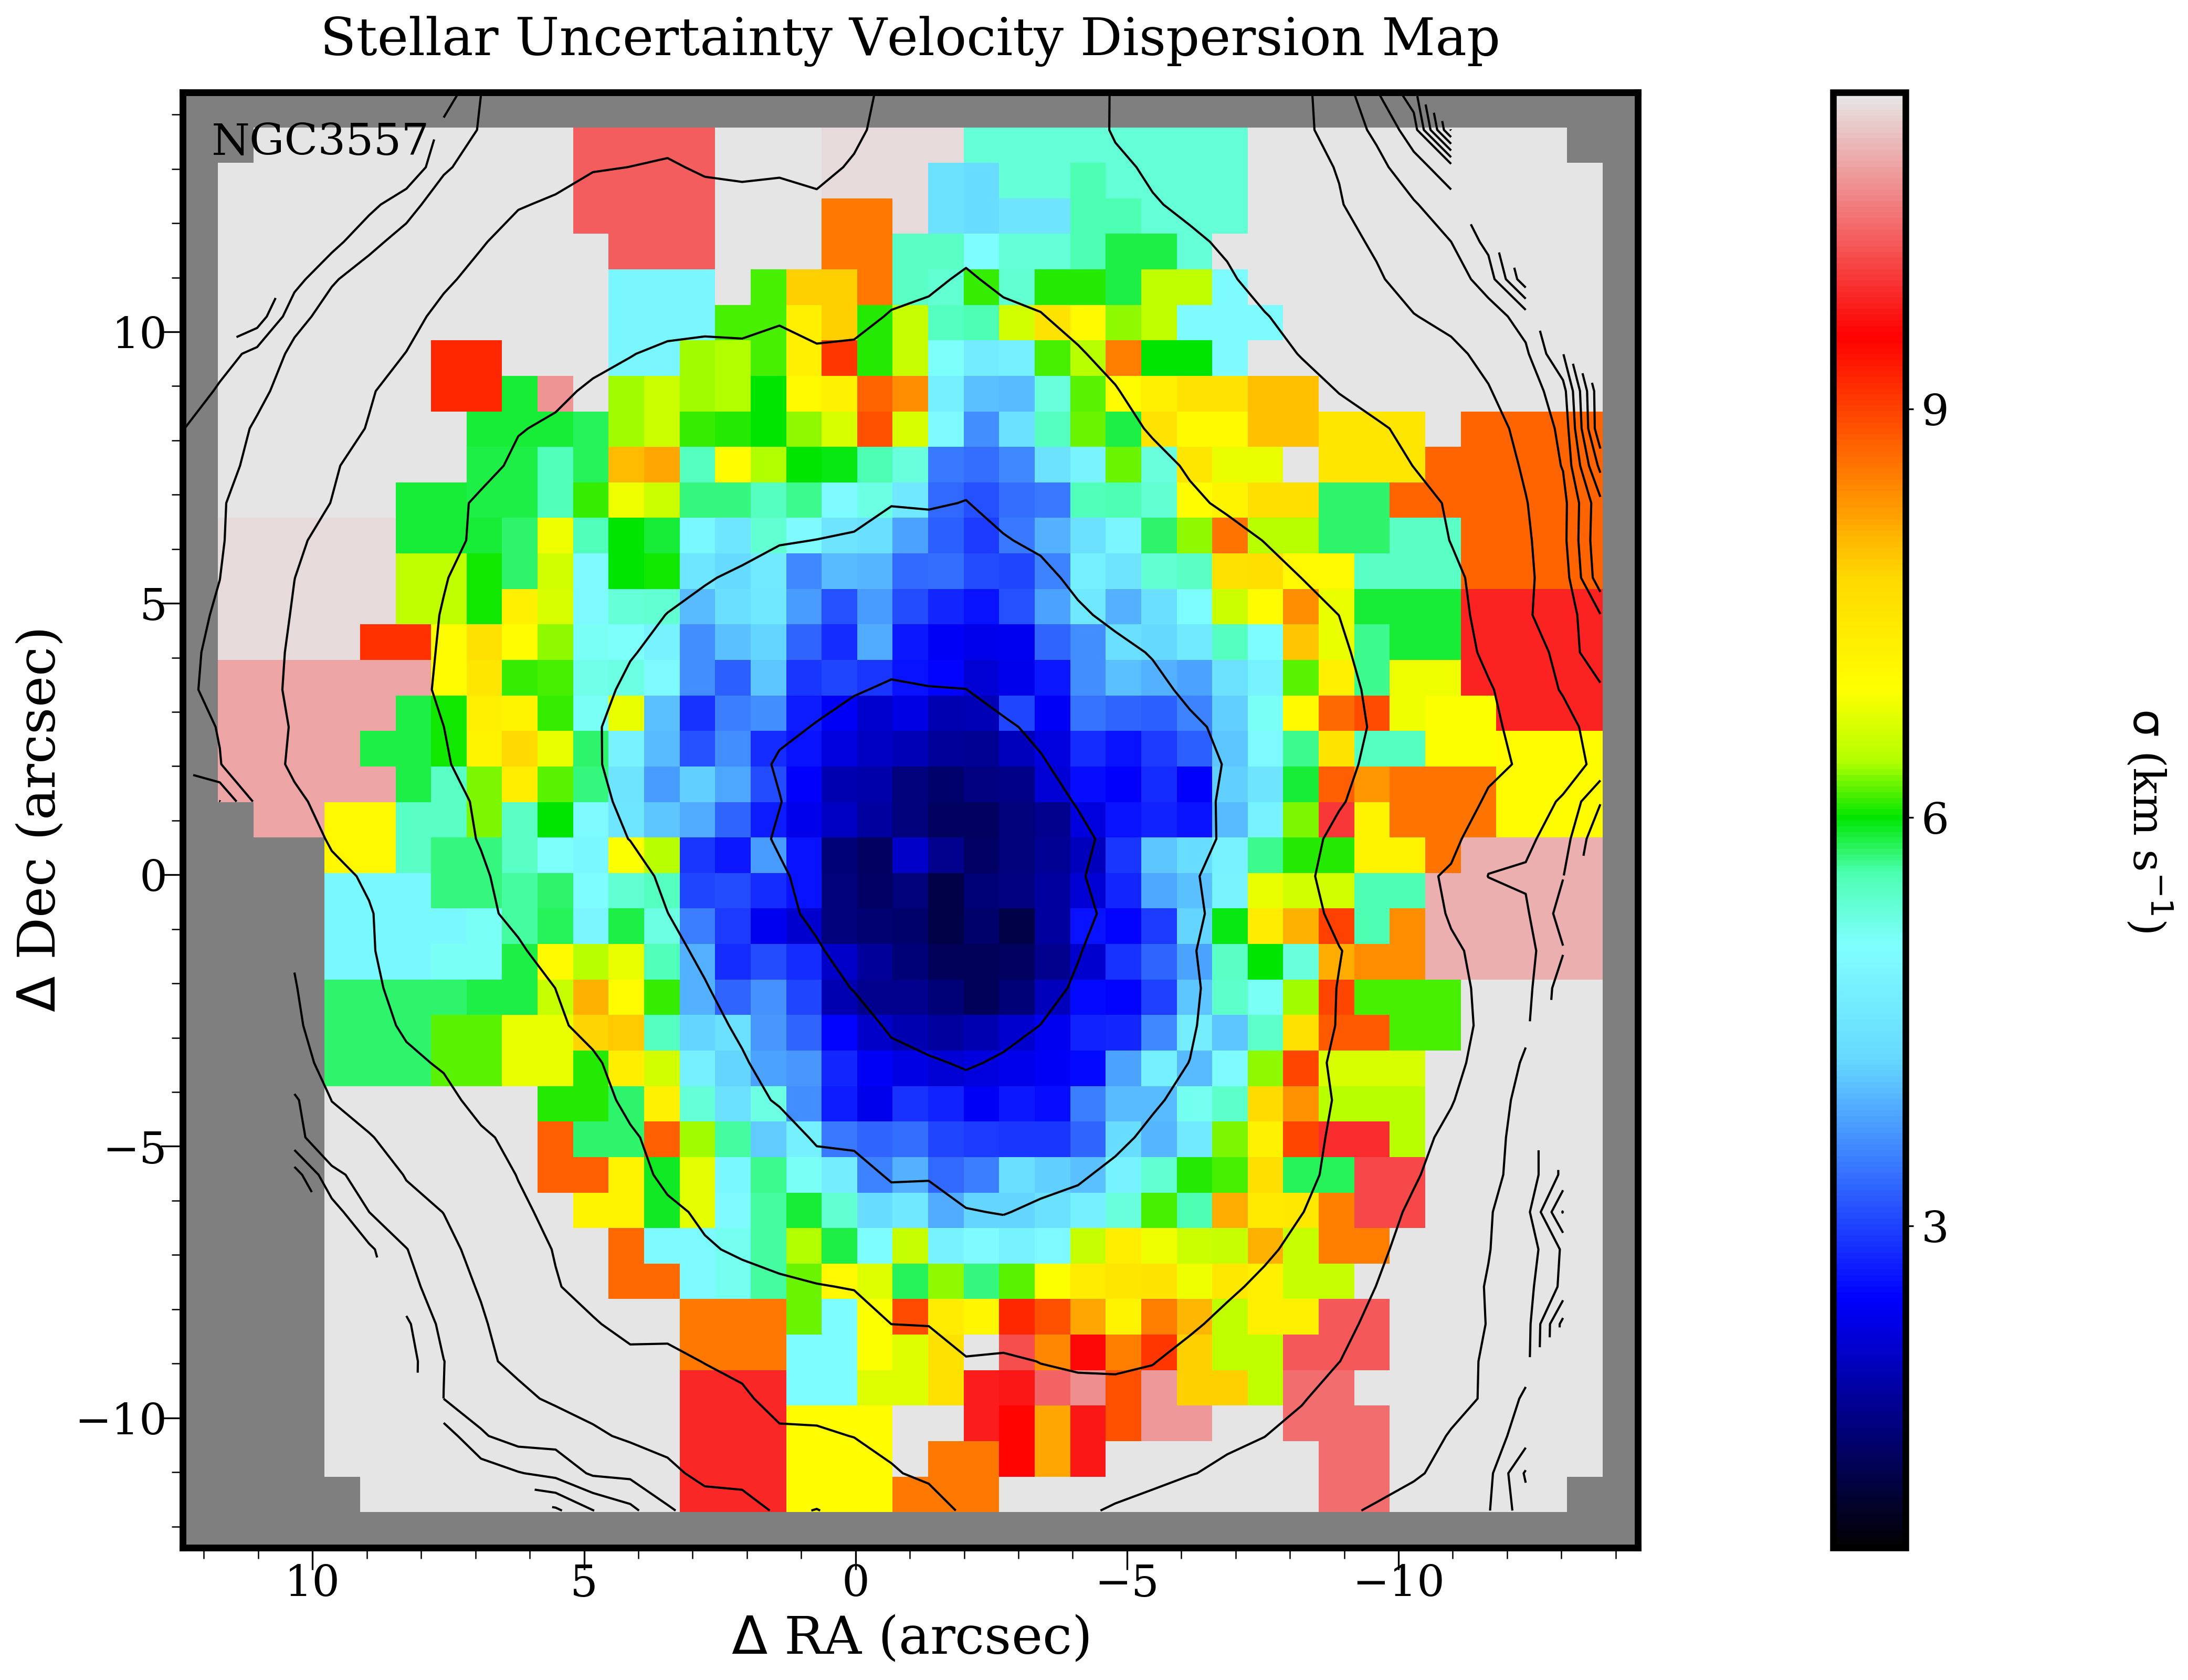
\includegraphics[width=0.245\textwidth]{Vmaps/ngc3557_stellar_sigma_uncert.png}
      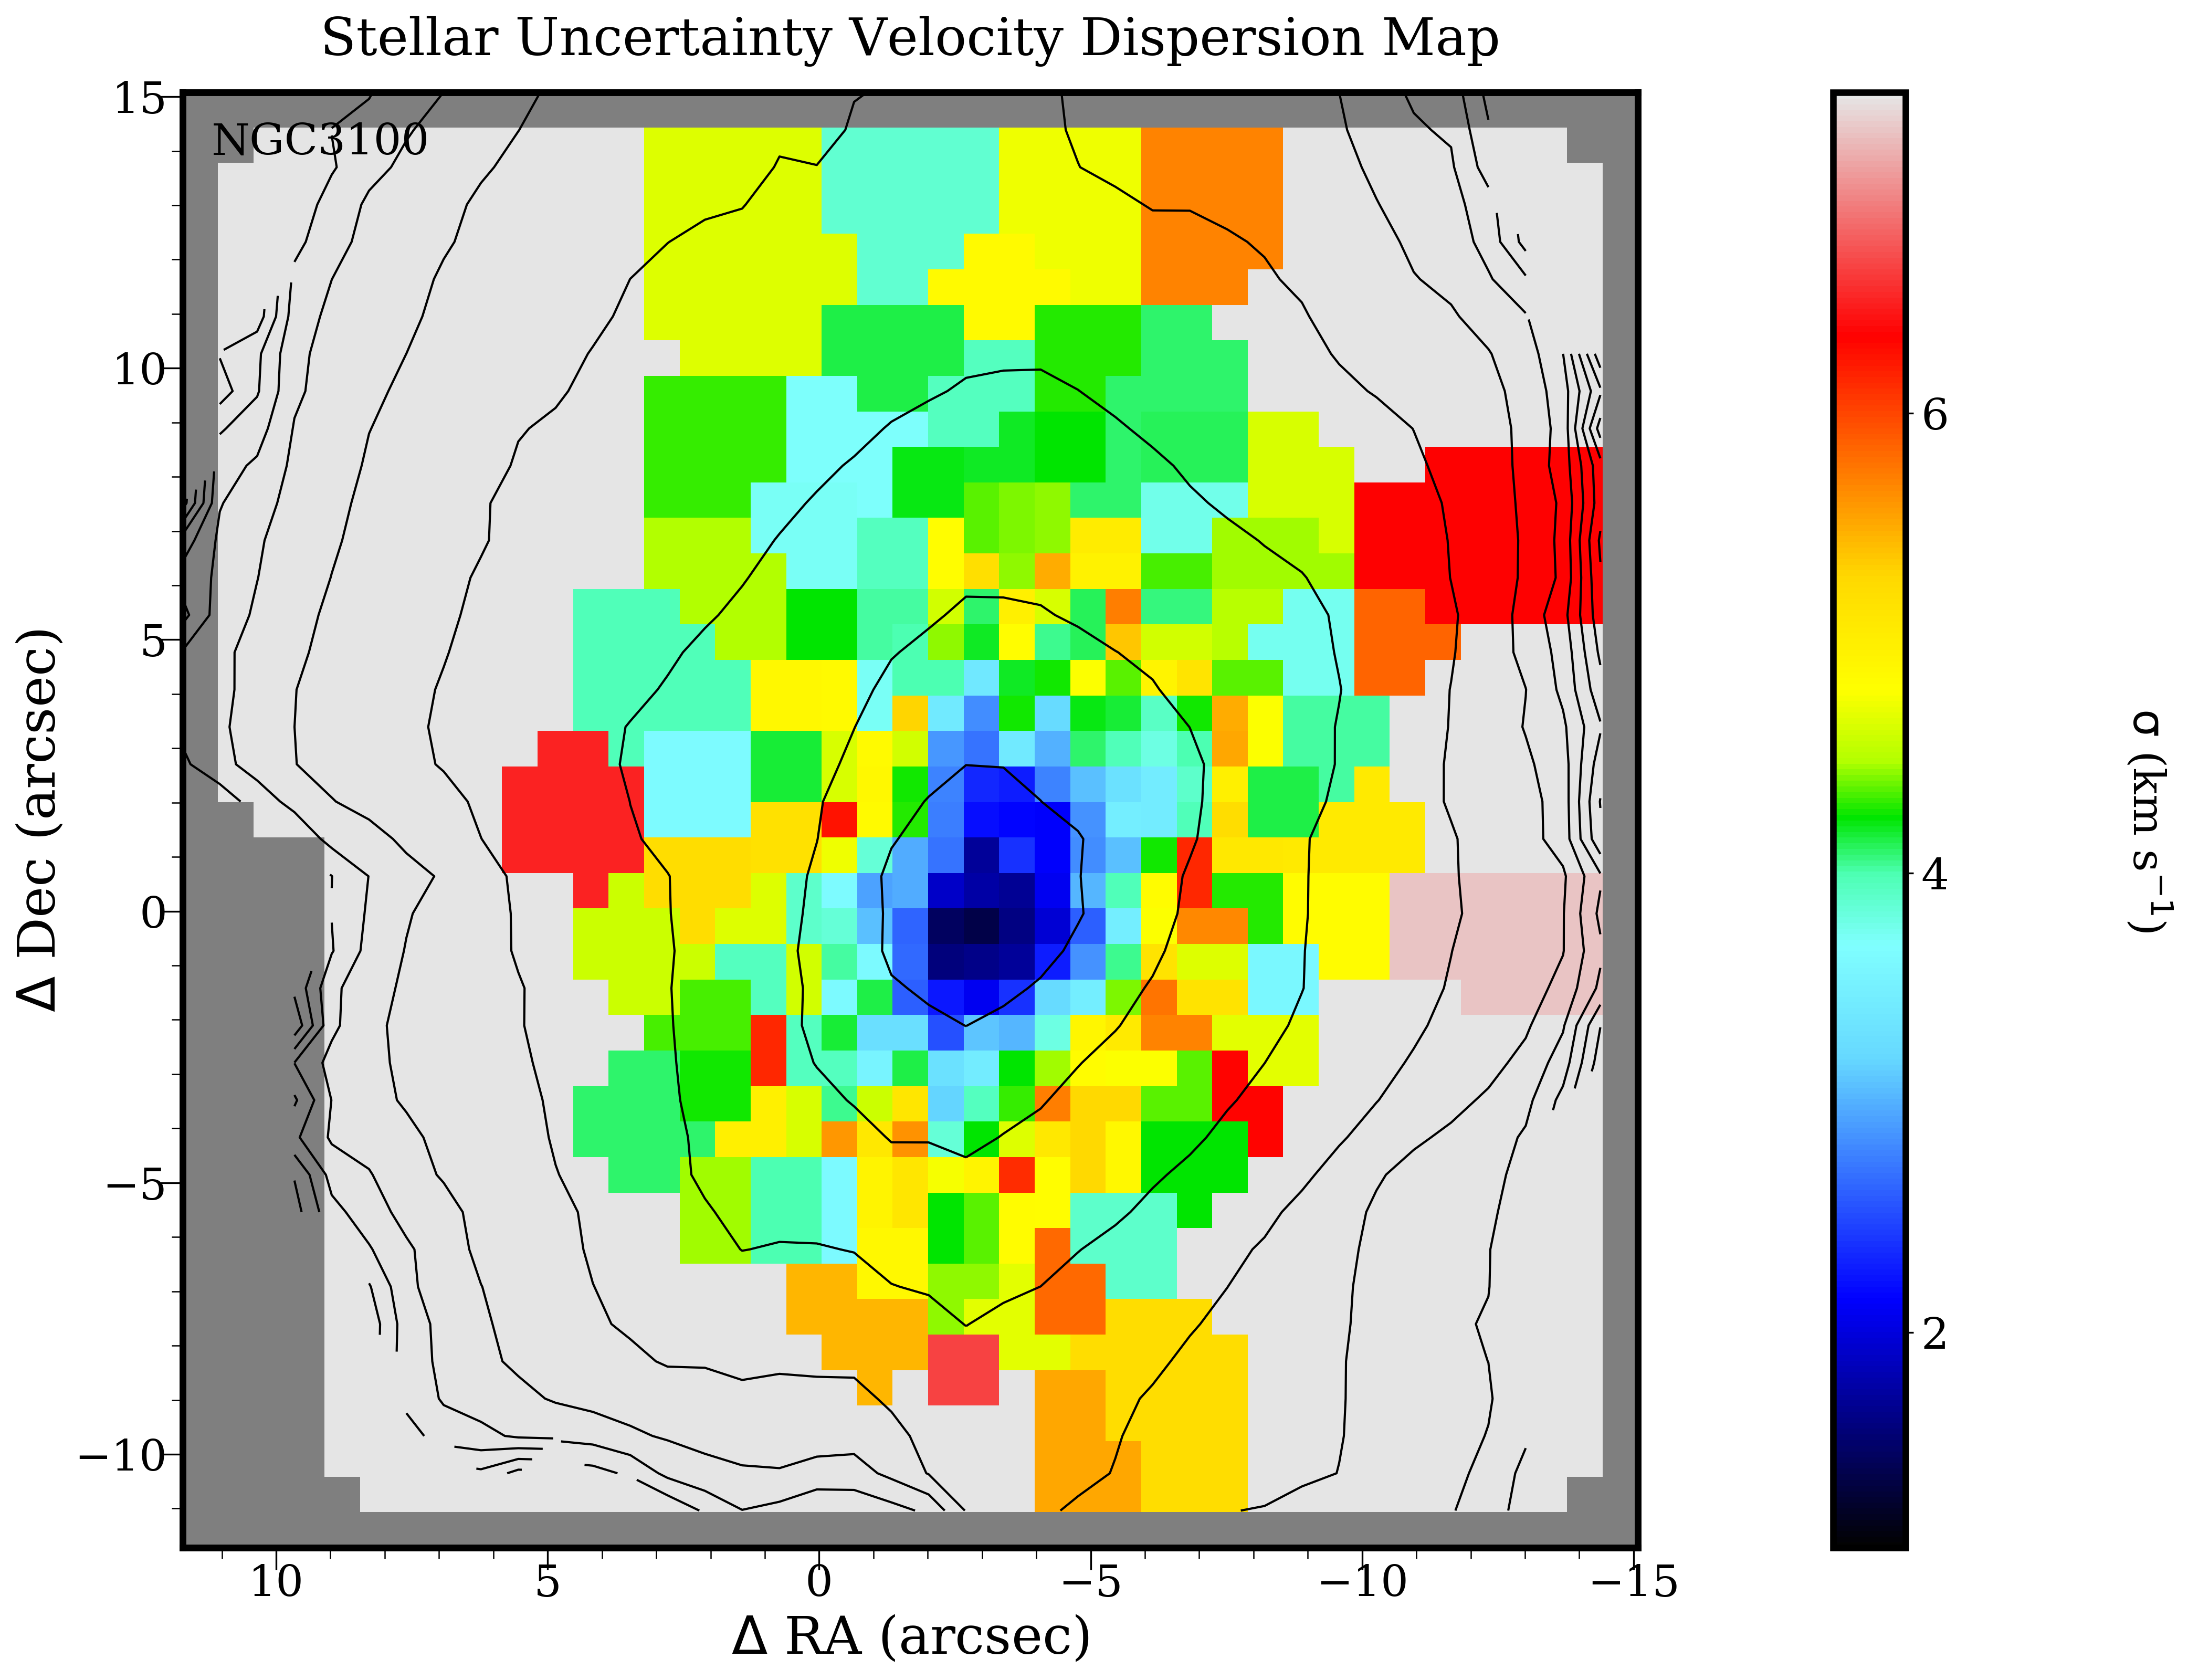
\includegraphics[width=0.245\textwidth]{Vmaps/ngc3100_stellar_sigma_uncert.png}
      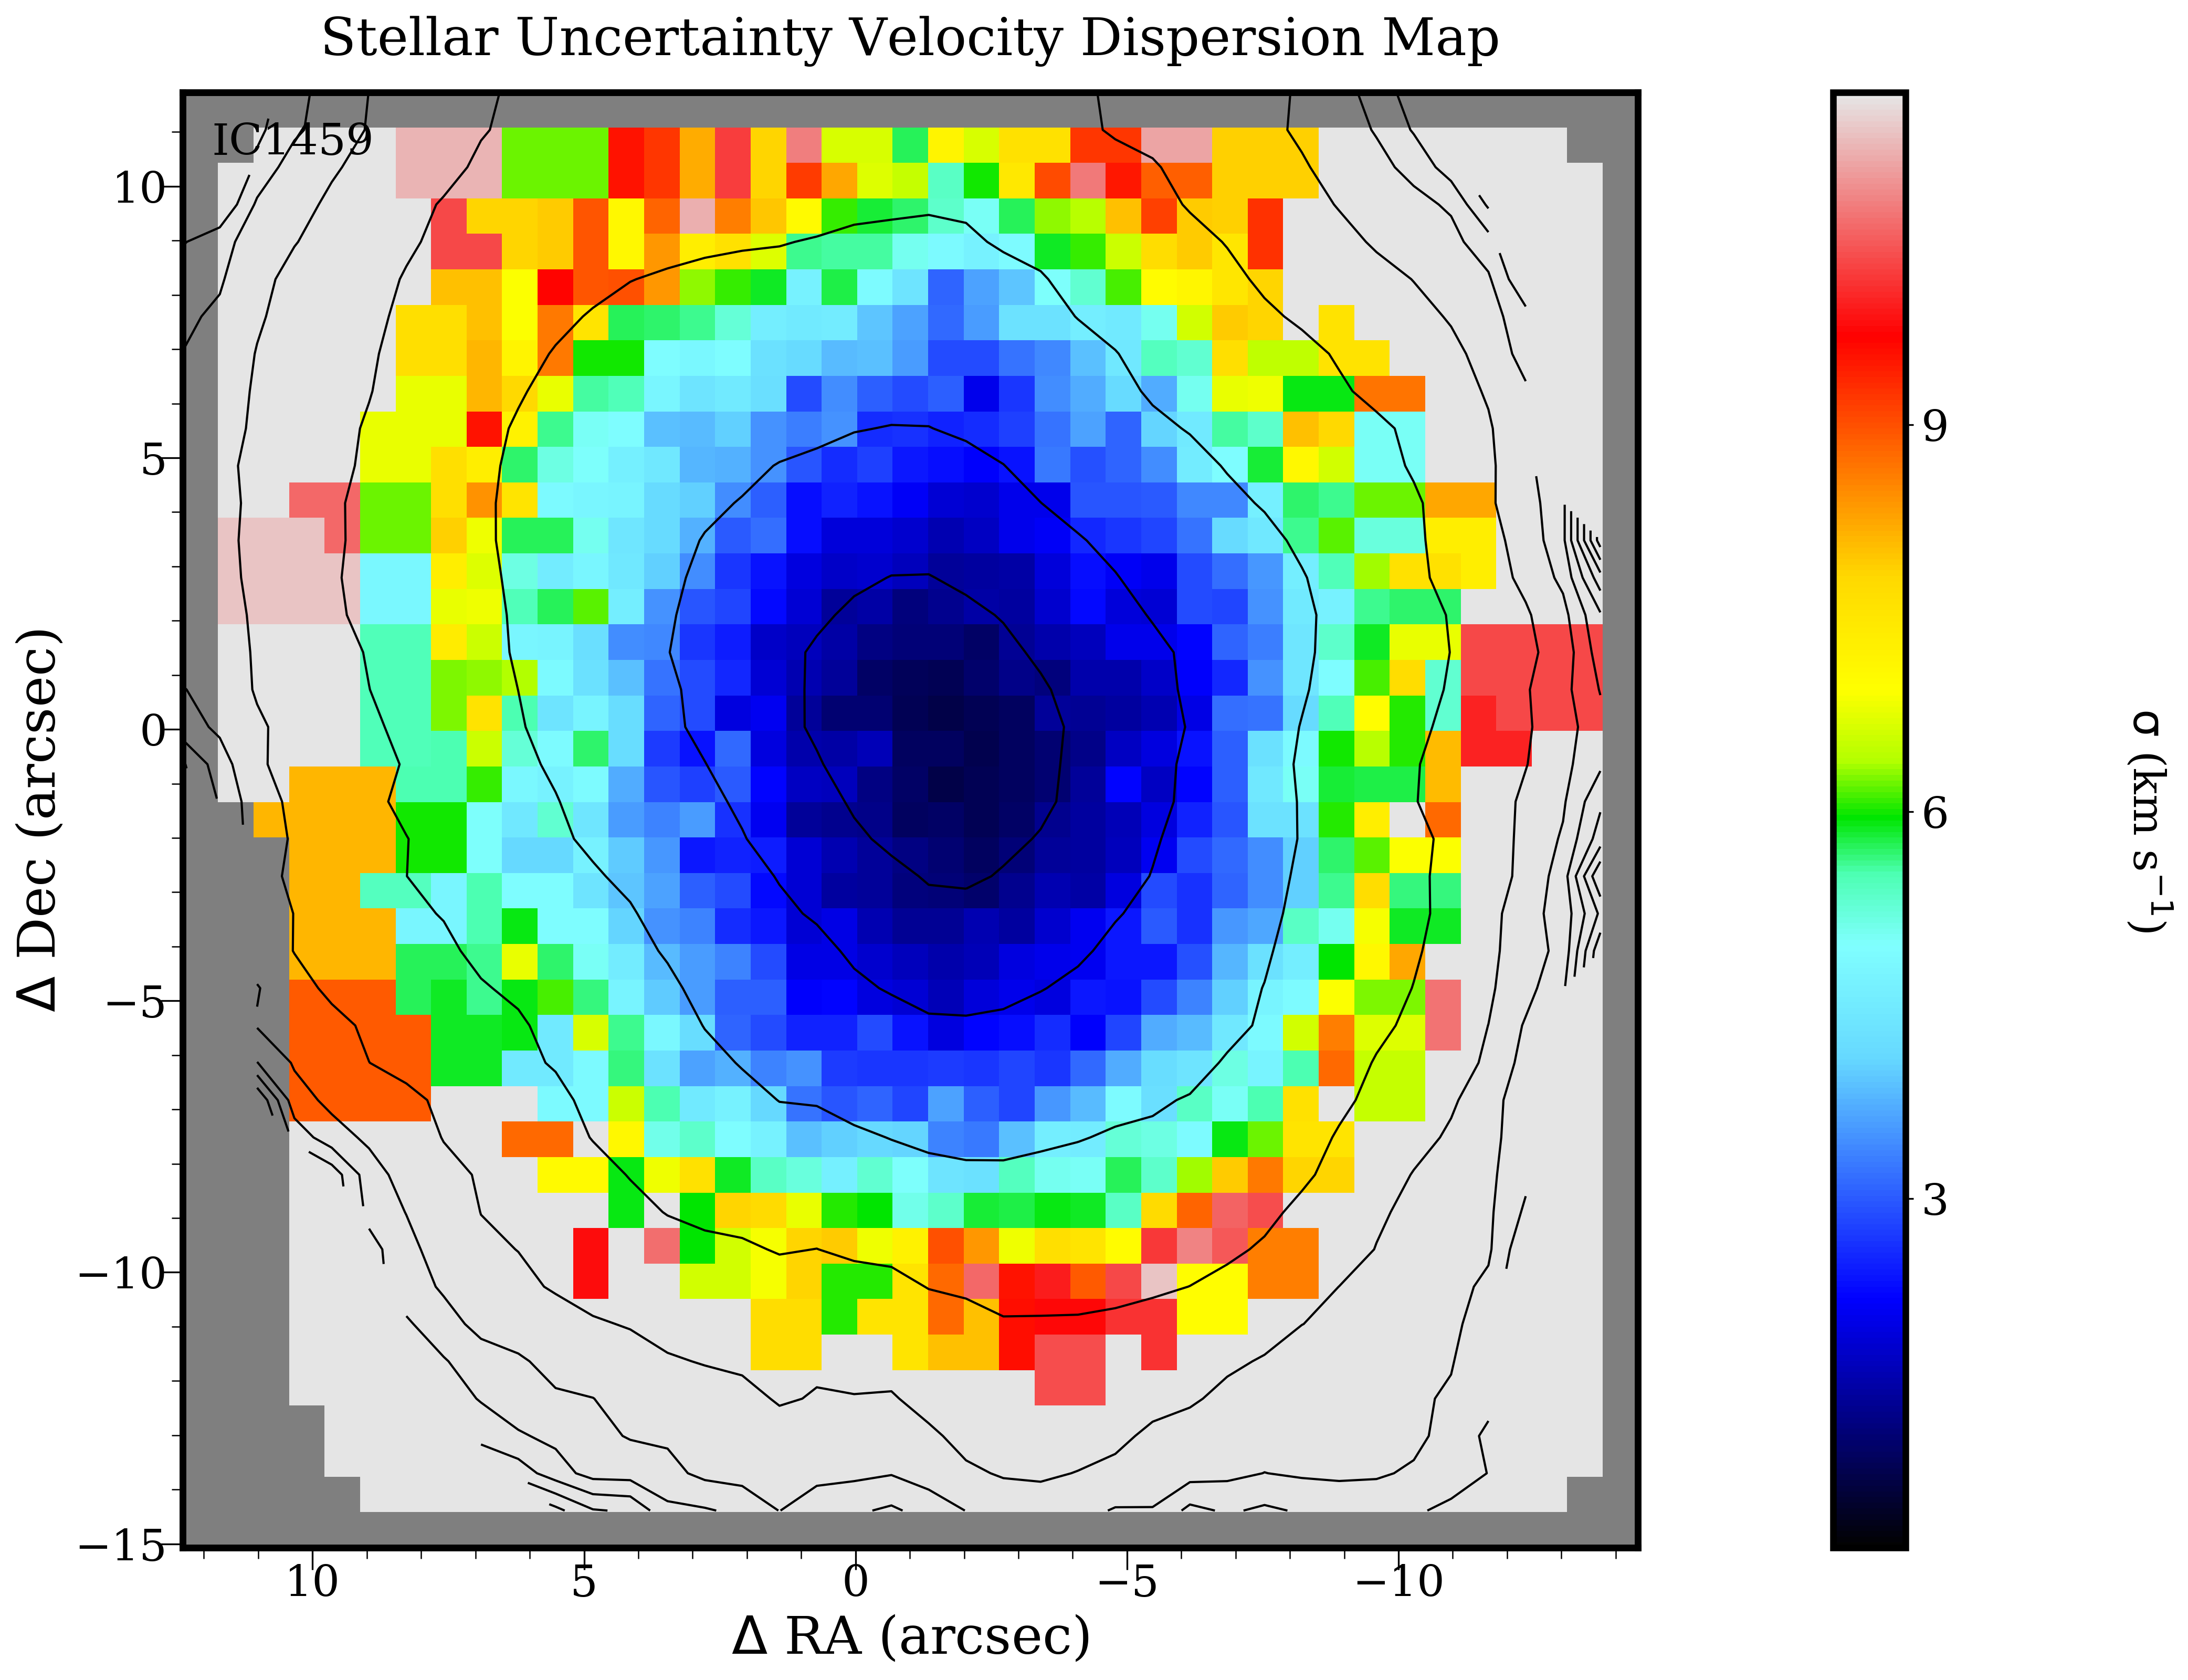
\includegraphics[width=0.245\textwidth]{Vmaps/ic1459_stellar_sigma_uncert.png}
      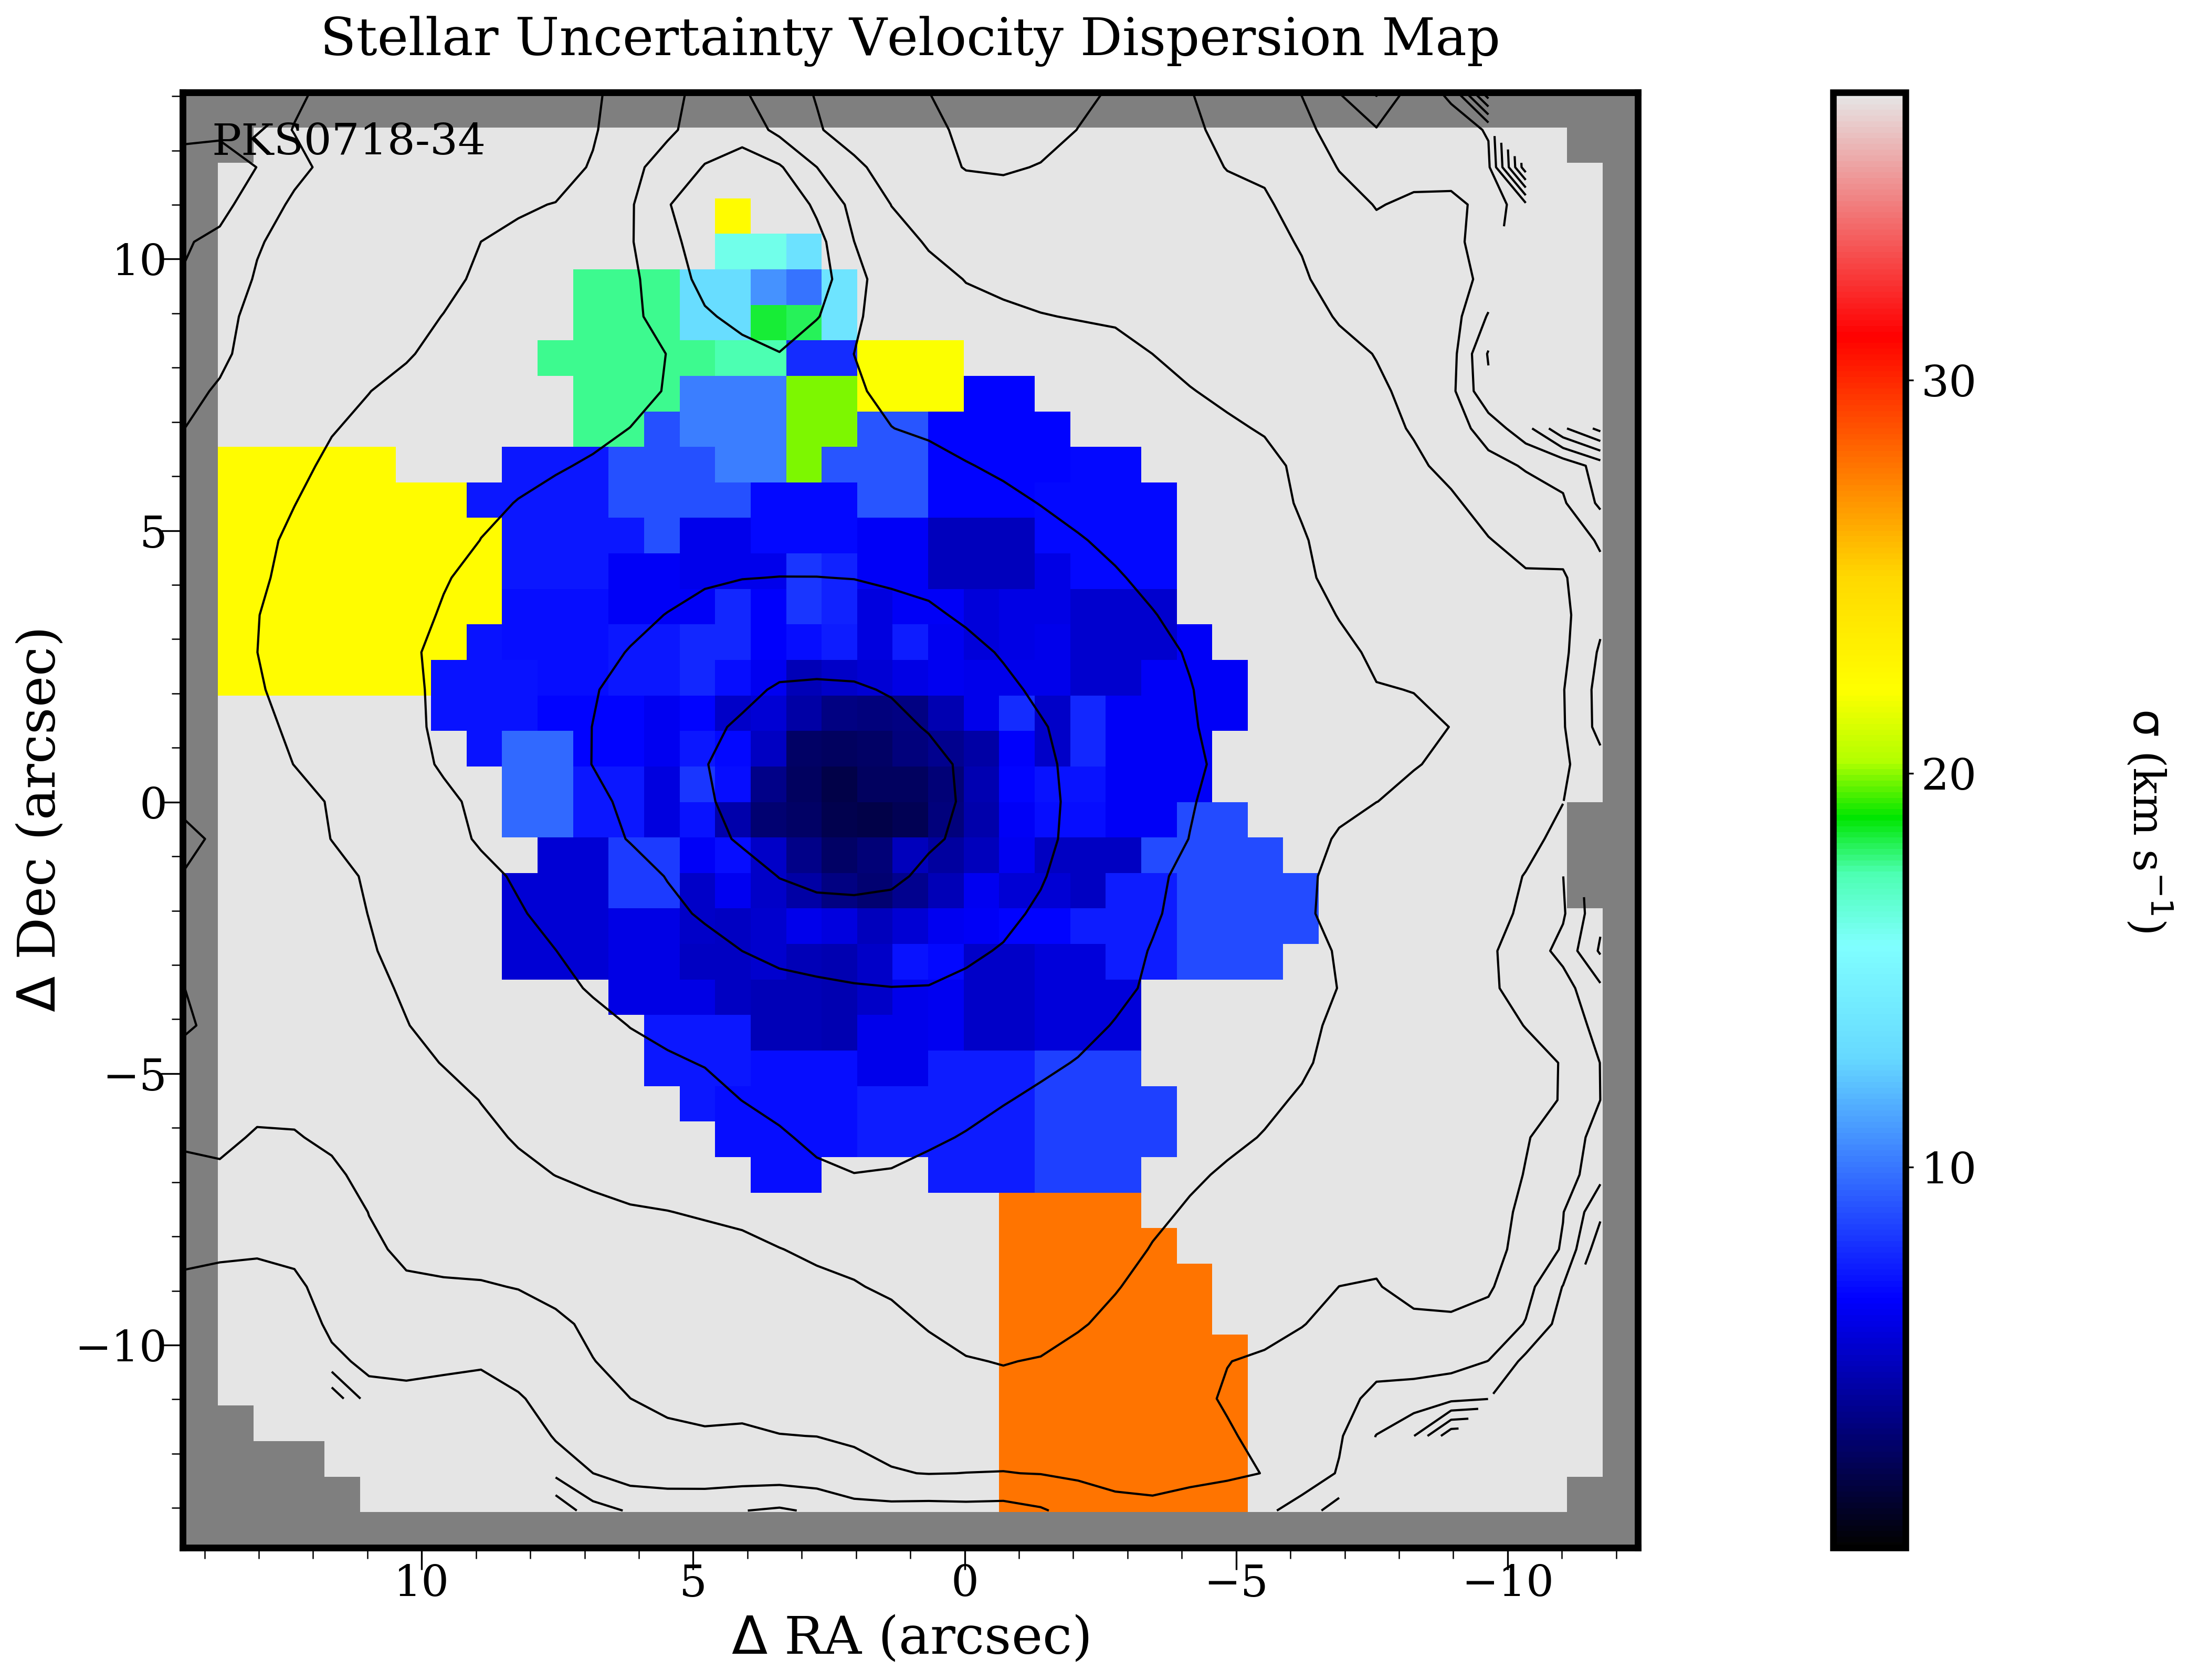
\includegraphics[width=0.245\textwidth]{Vmaps/pks0718-34_stellar_sigma_uncert.png}
      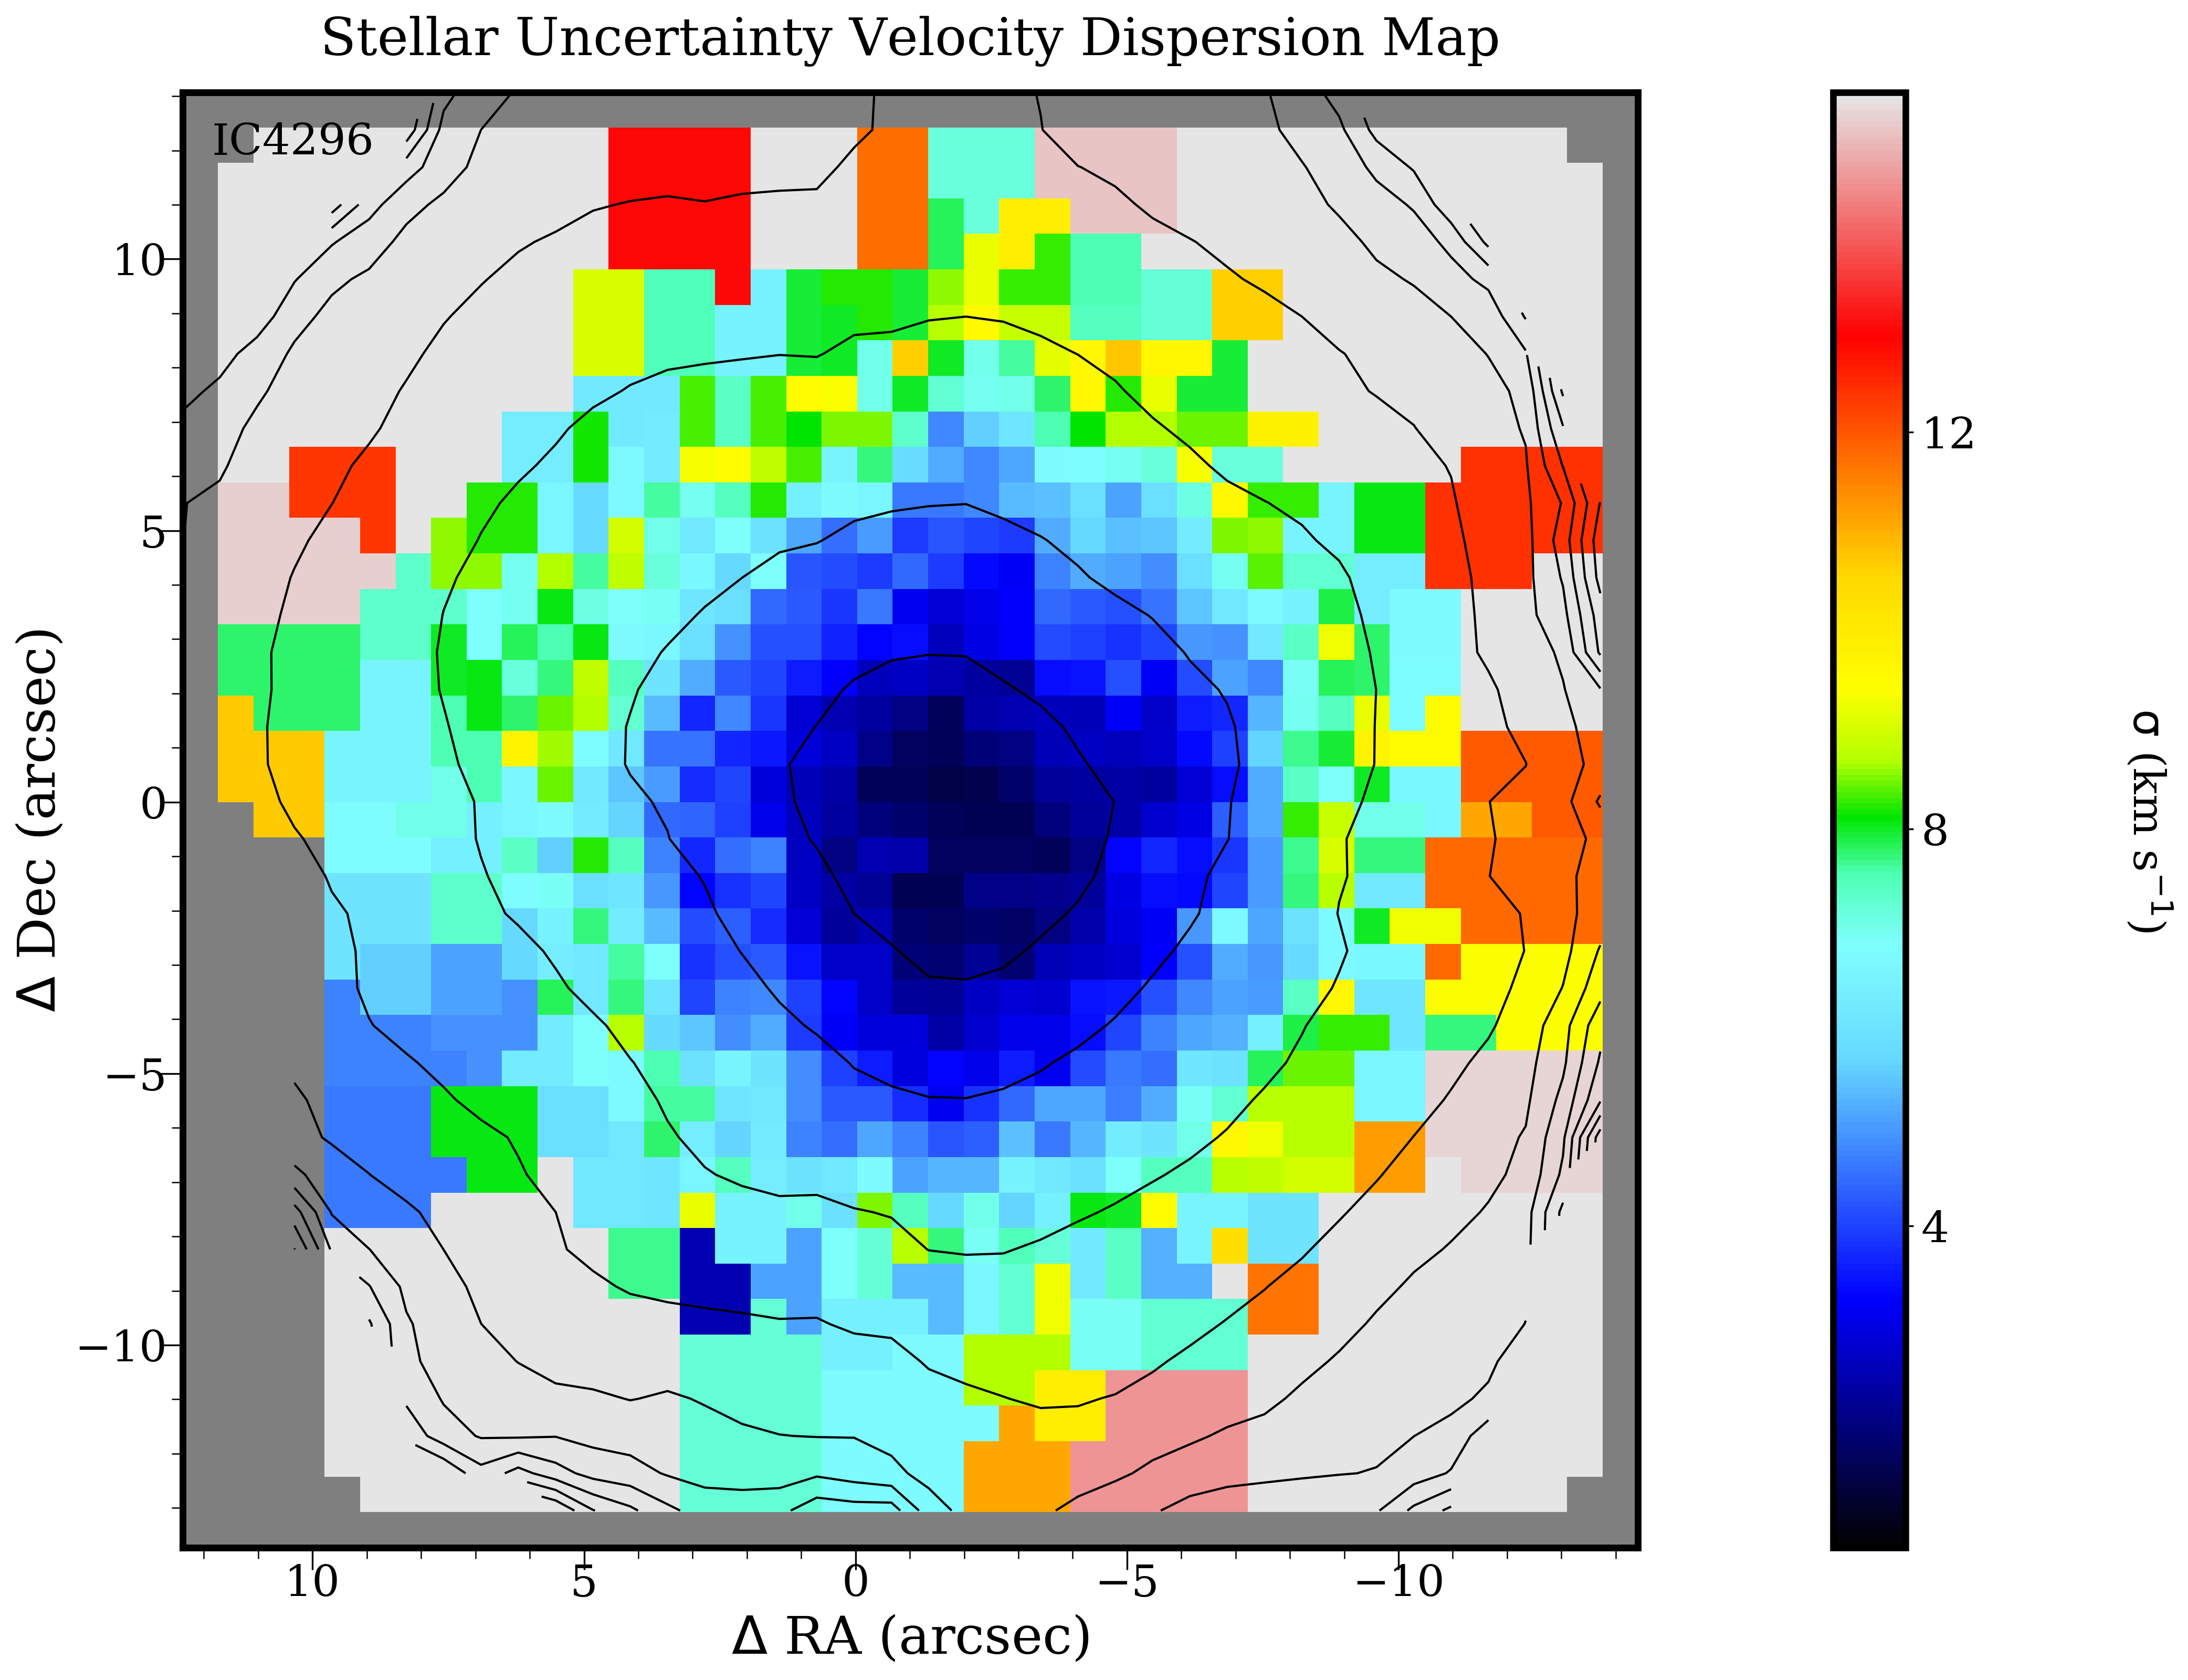
\includegraphics[width=0.245\textwidth]{Vmaps/ic4296_stellar_sigma_uncert.png}
      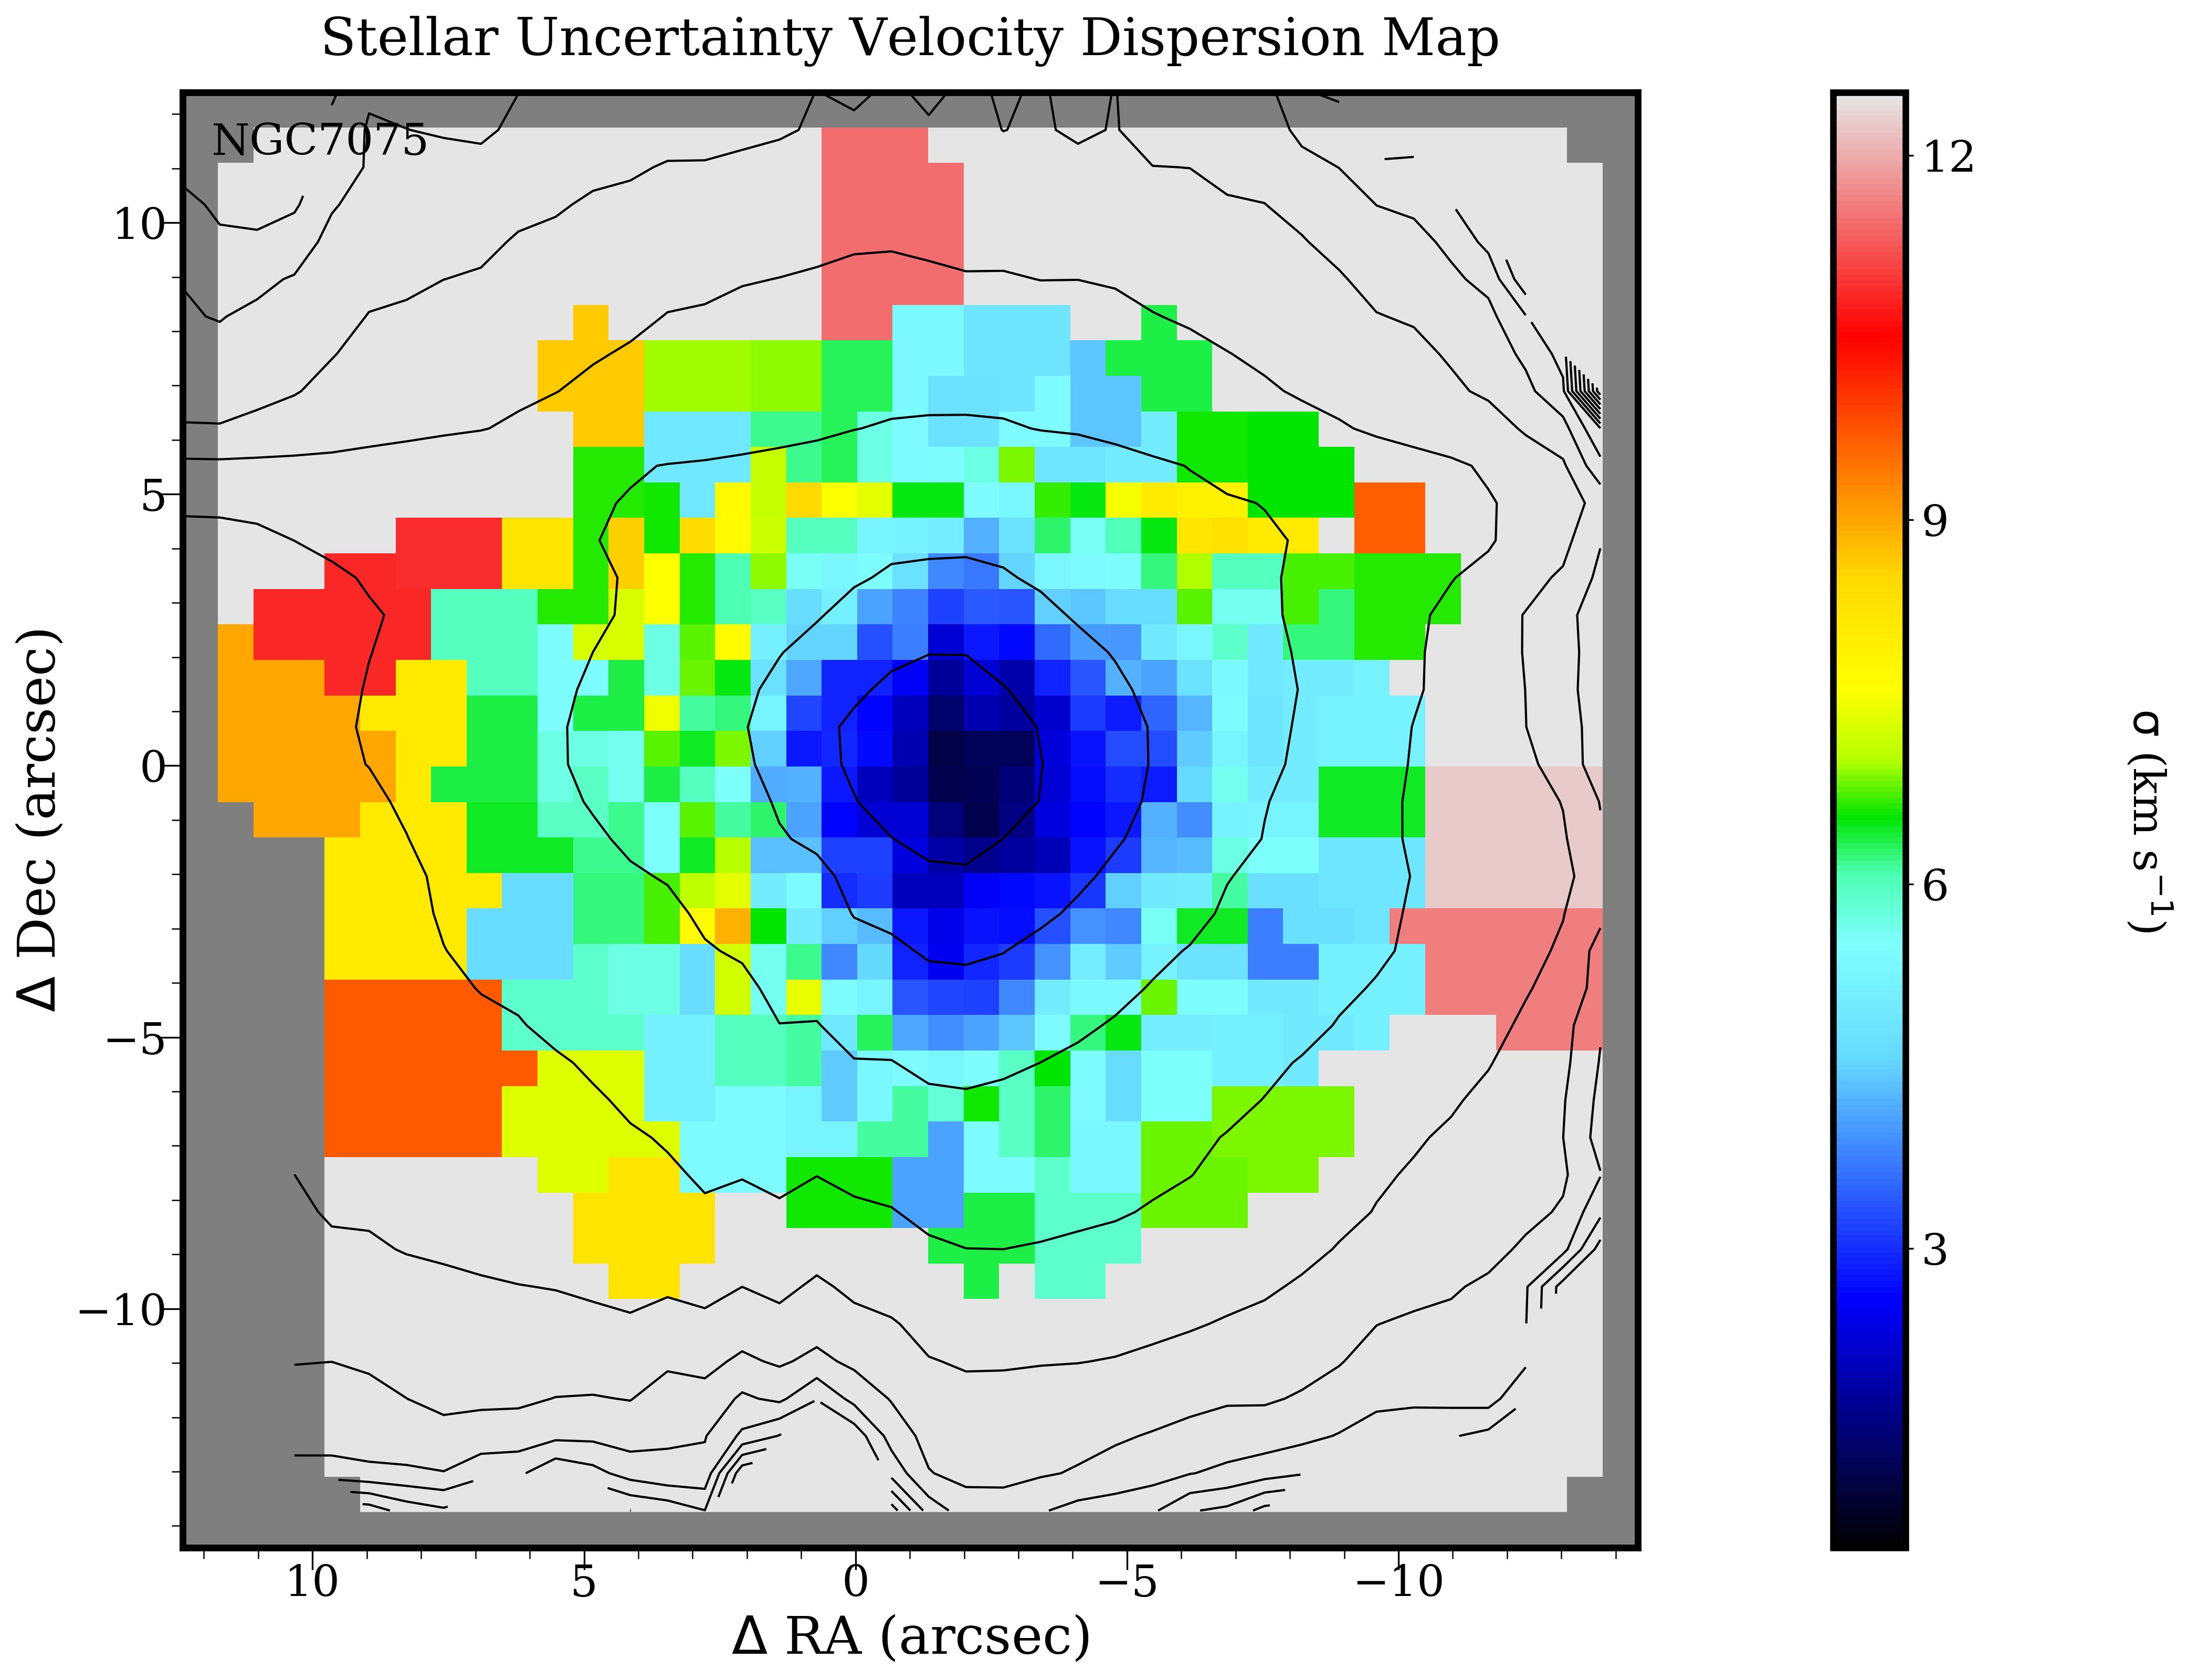
\includegraphics[width=0.245\textwidth]{Vmaps/ngc7075_stellar_sigma_uncert.png}
      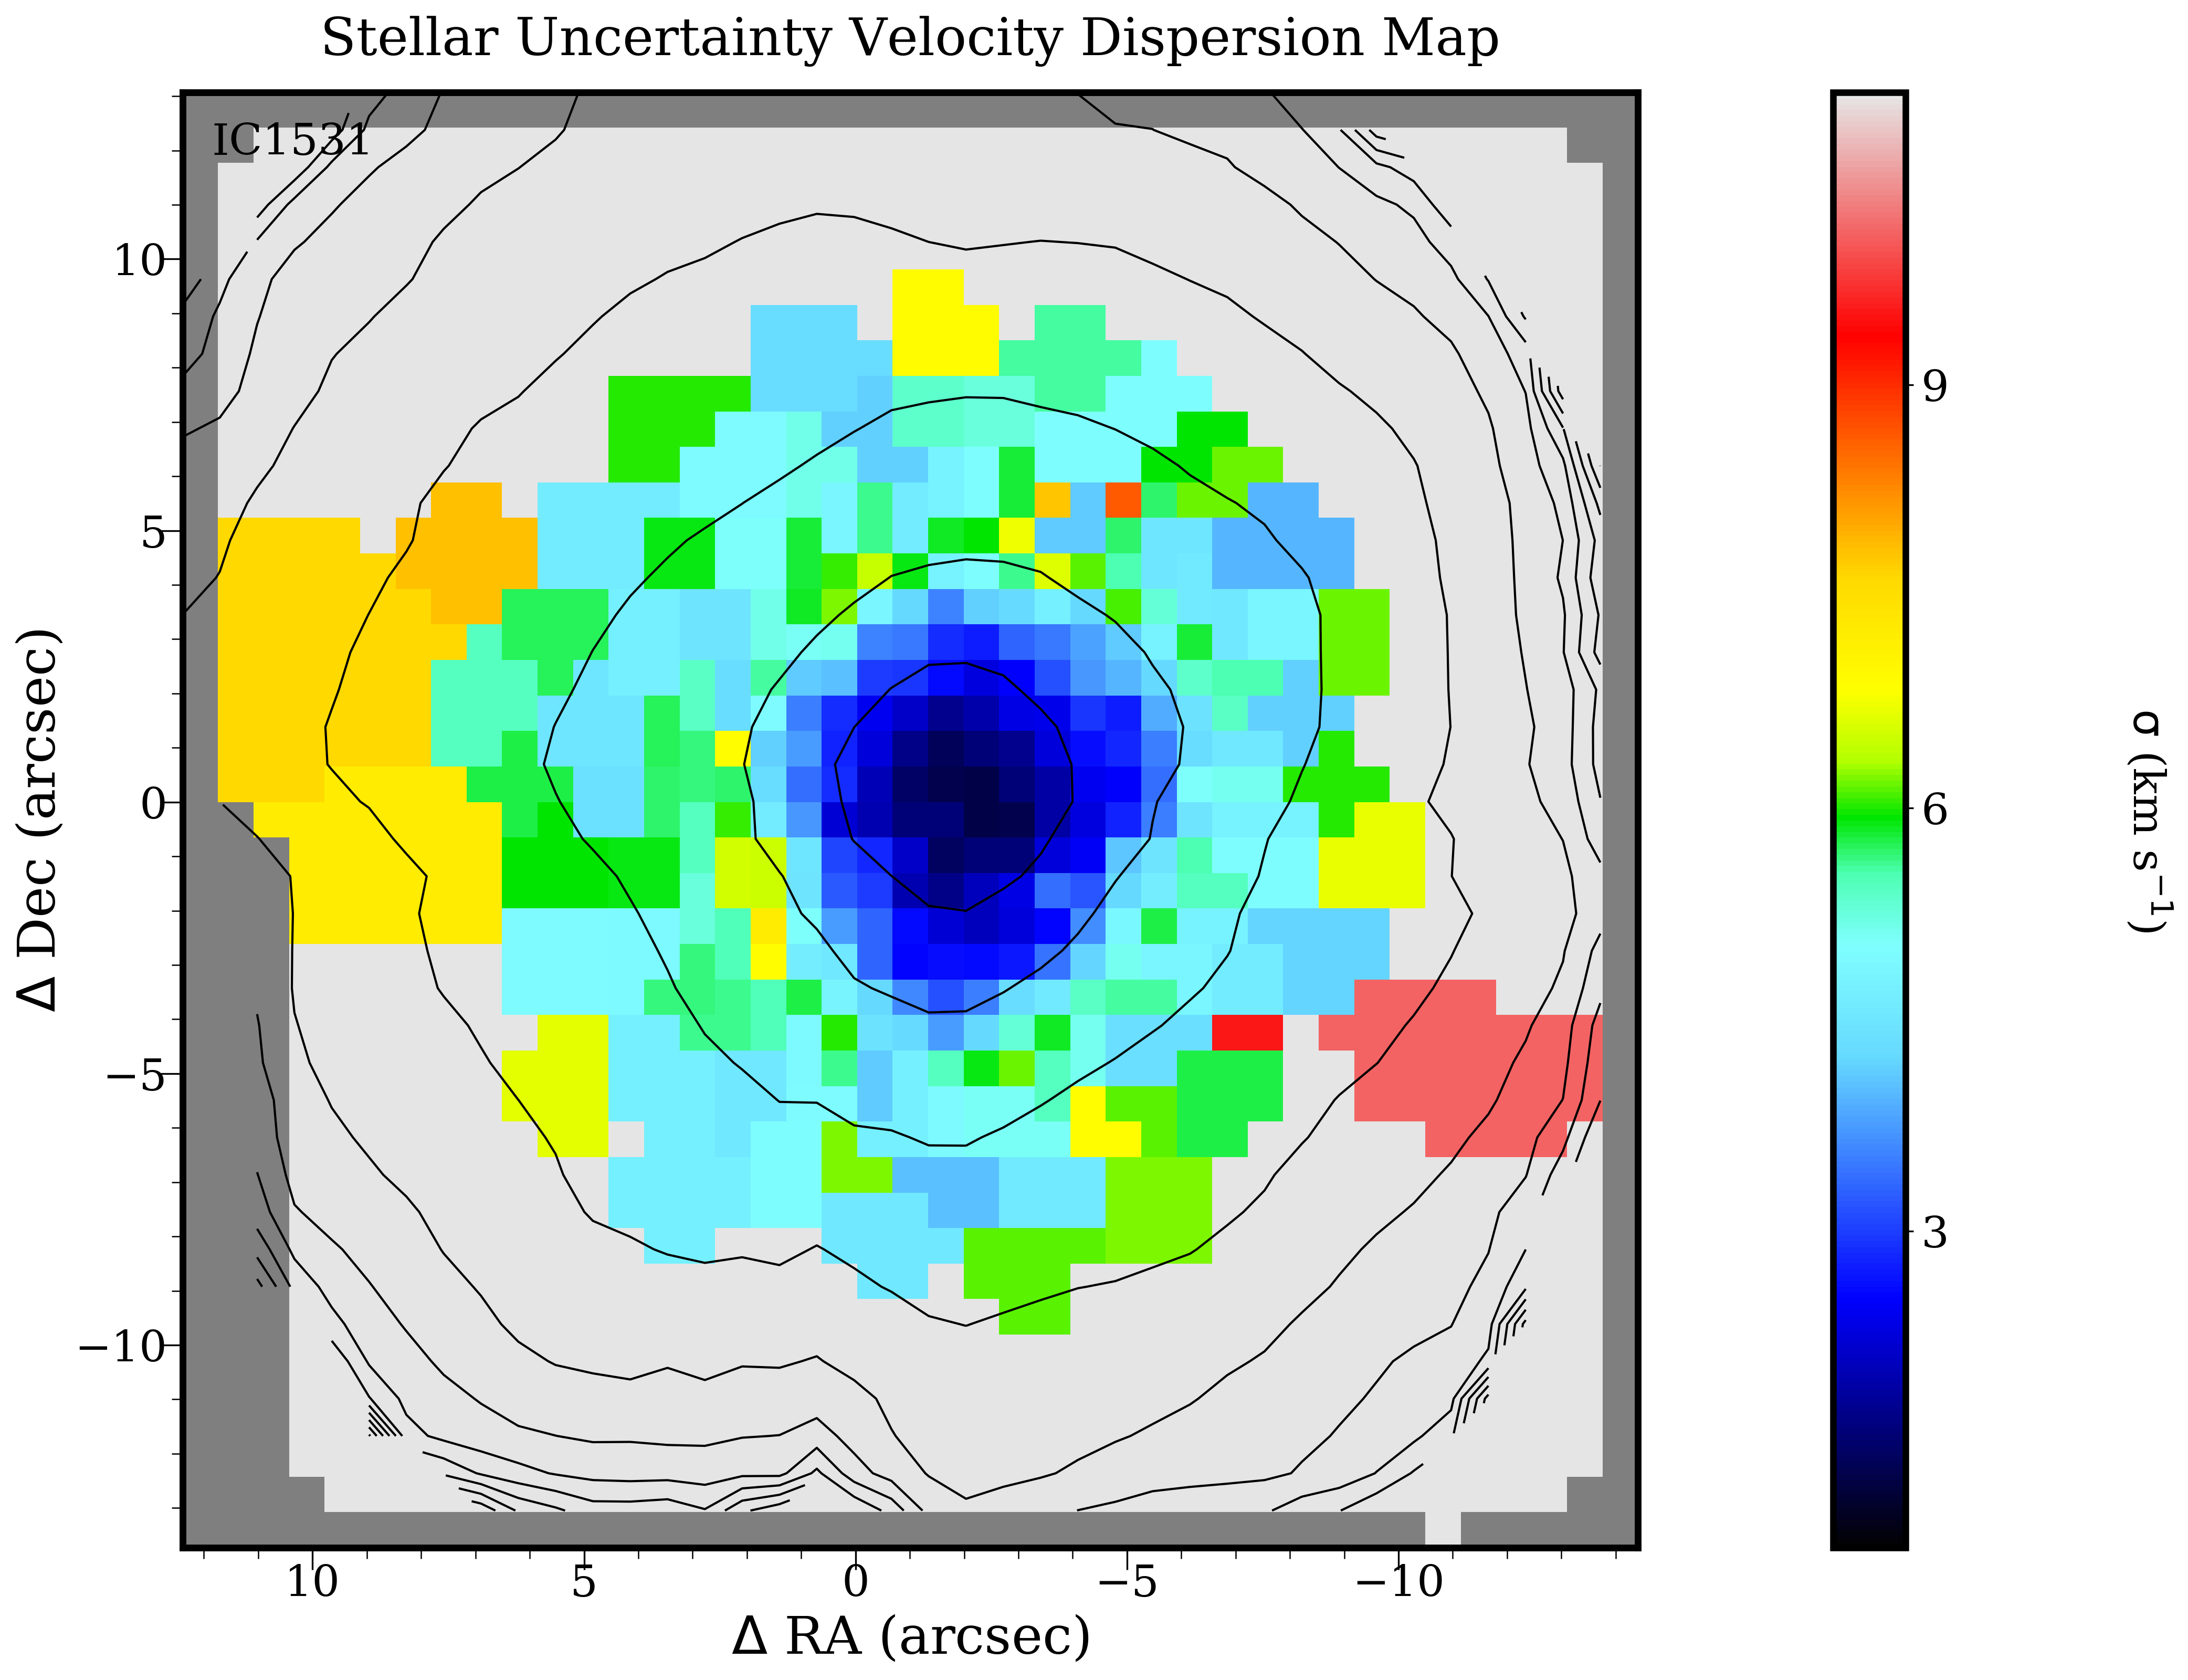
\includegraphics[width=0.245\textwidth]{Vmaps/ic1531_stellar_sigma_uncert.png}
      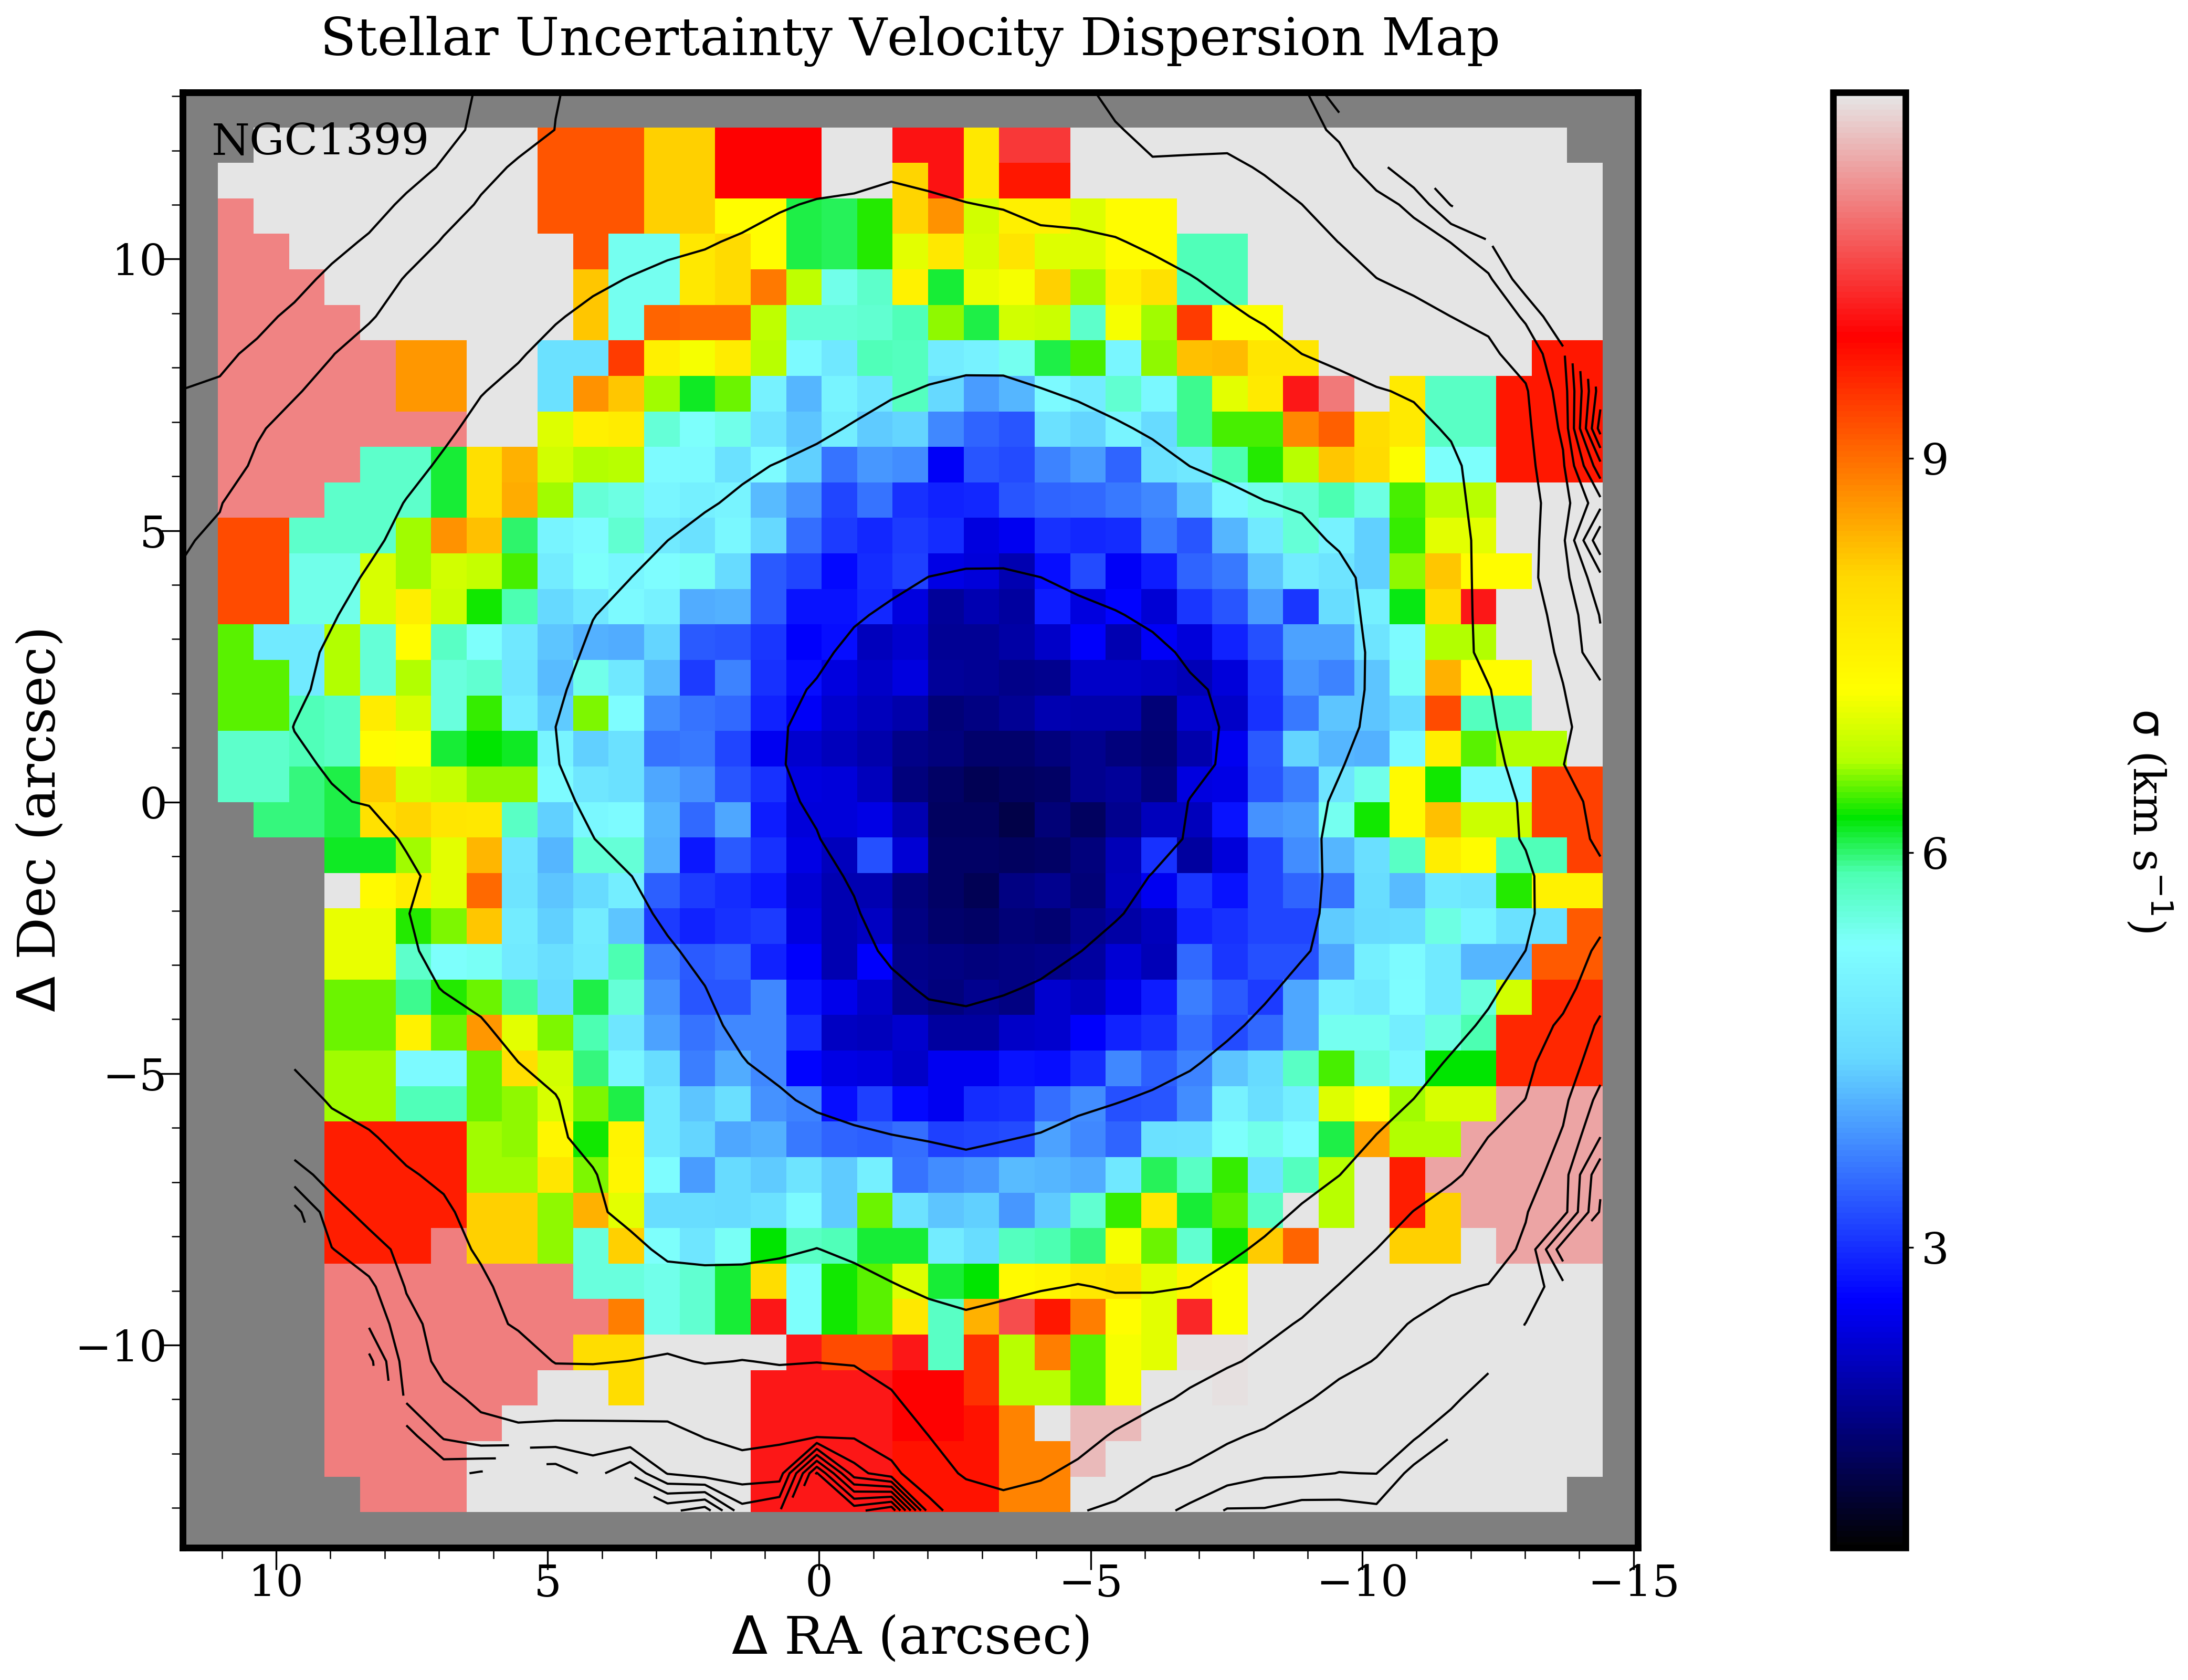
\includegraphics[width=0.245\textwidth]{Vmaps/ngc1399_stellar_sigma_uncert.png}
      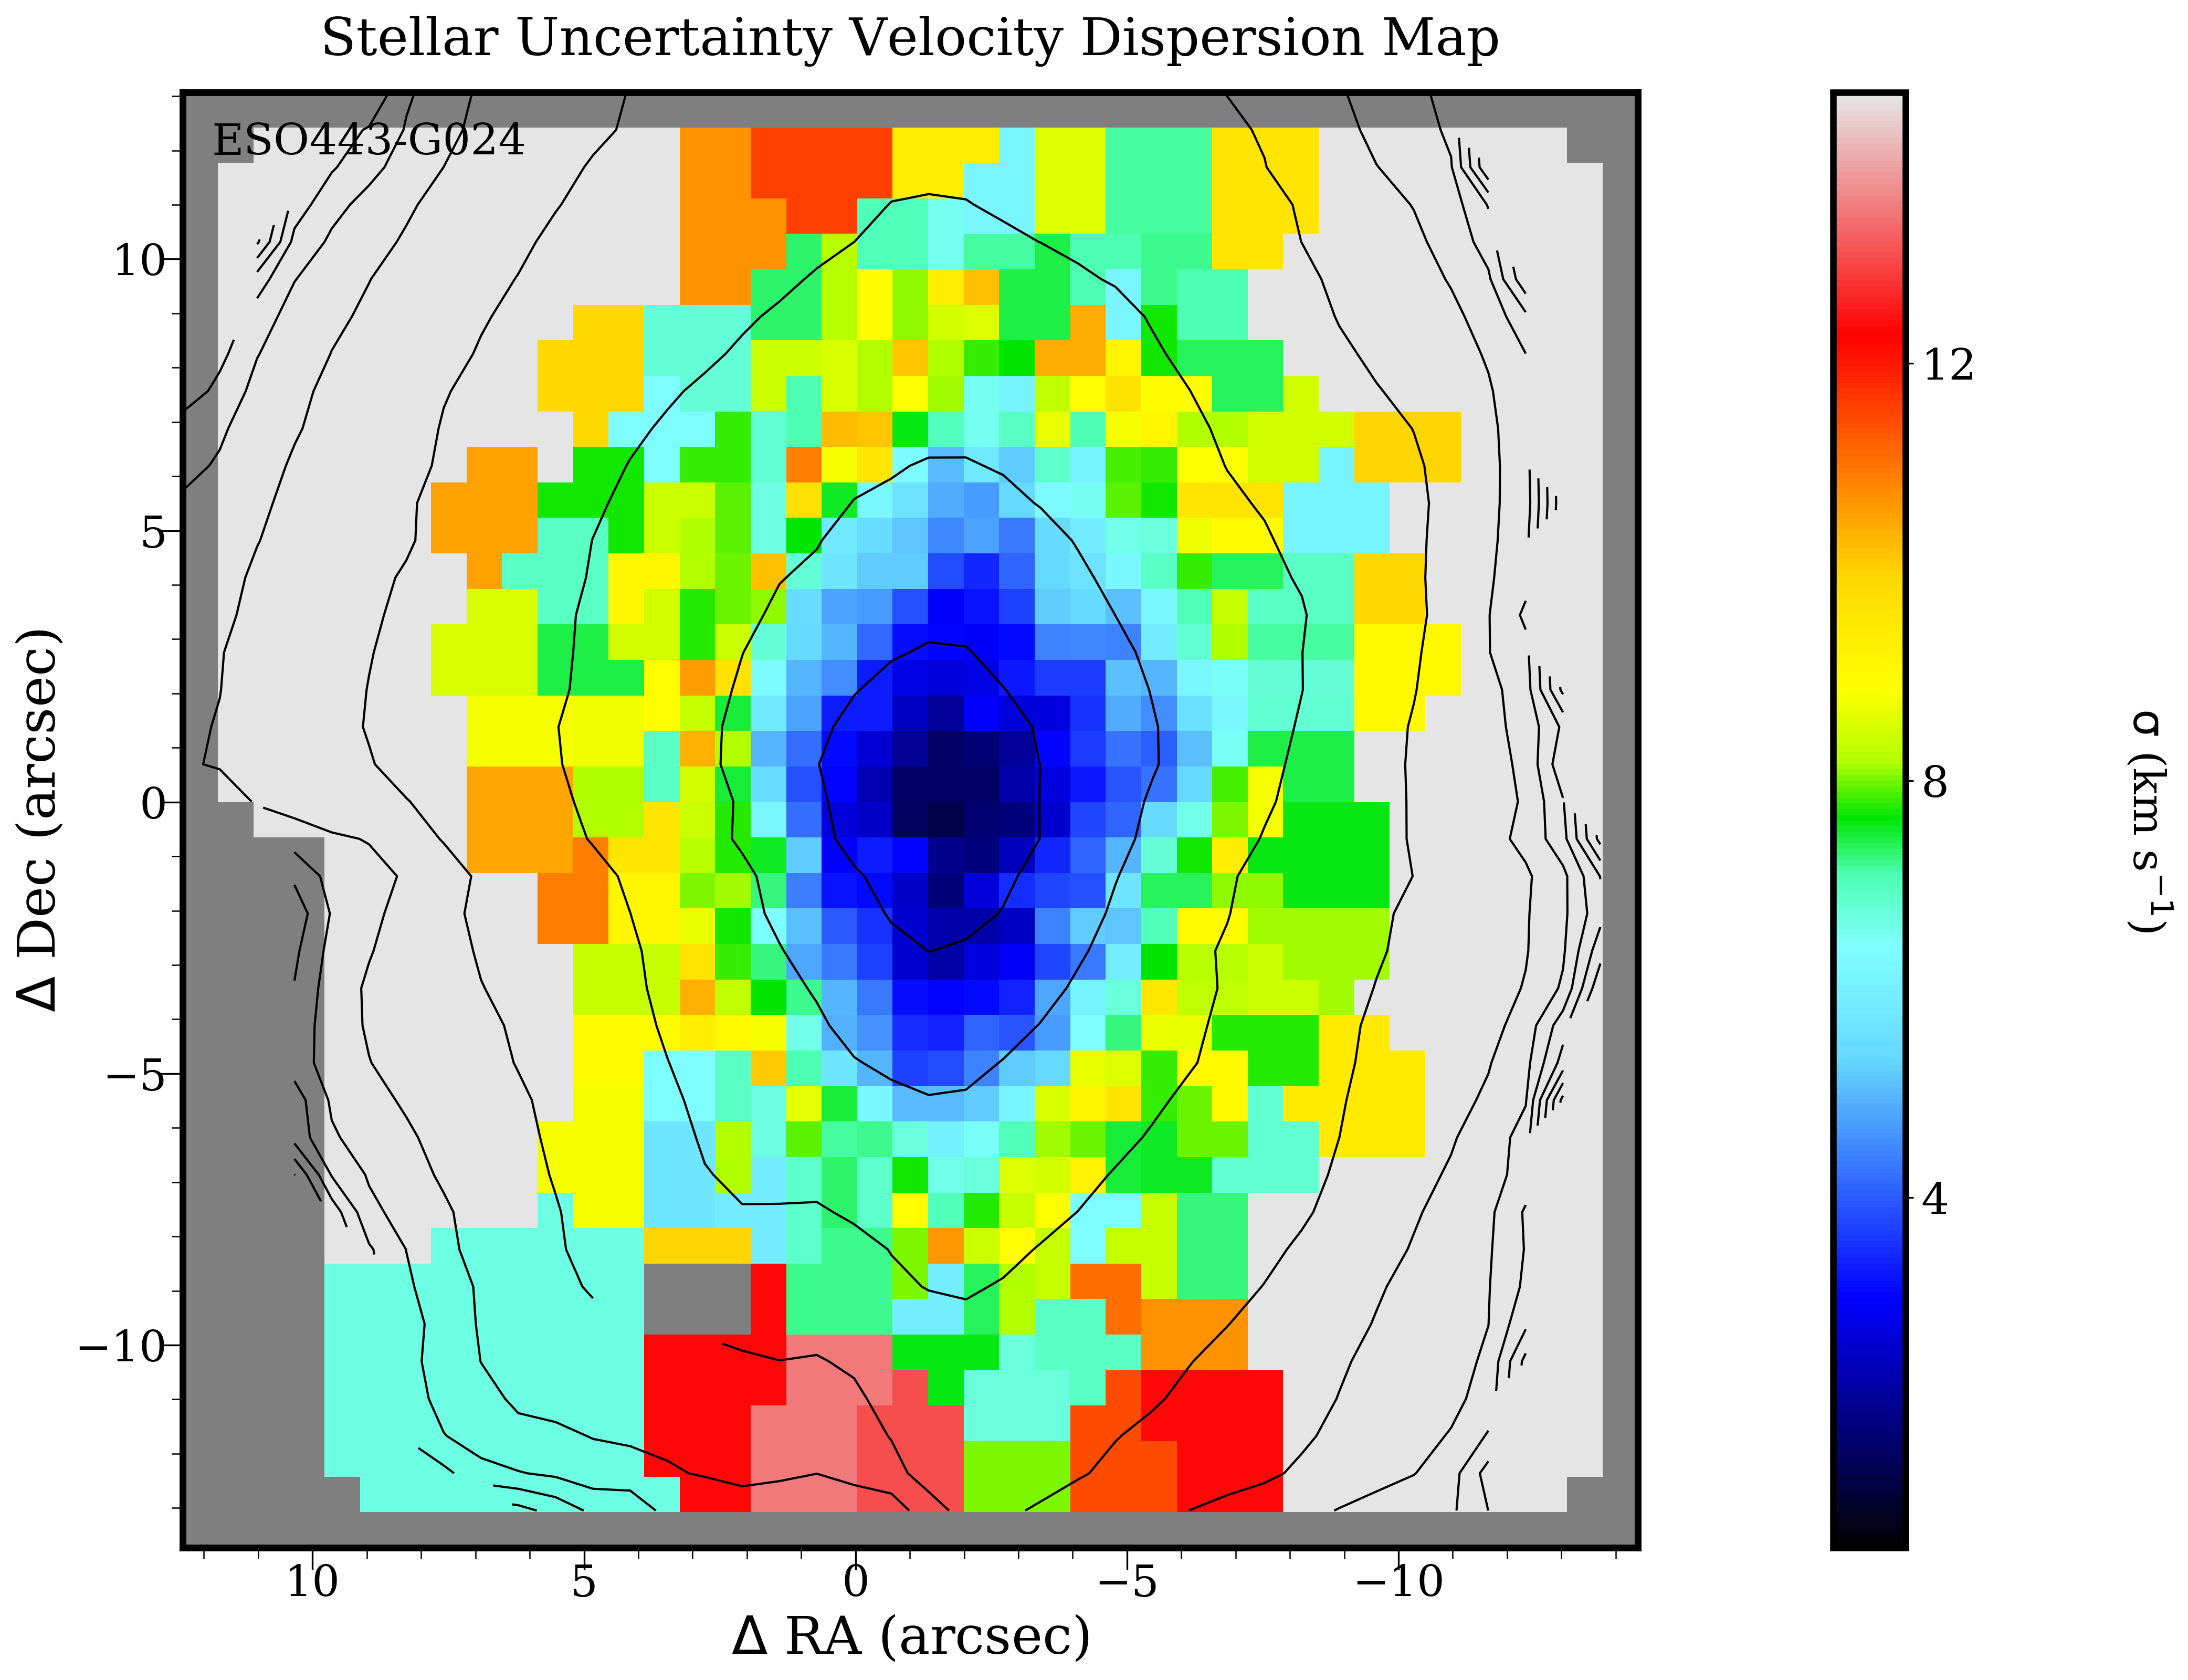
\includegraphics[width=0.245\textwidth]{Vmaps/eso443-g024_stellar_sigma_uncert.png}
      \caption[VIMOS dispersion uncertocity maps]{Uncertainties in the velocity dispersion for each galaxy in the VIMOS sample. Plots are ordered and contour colors are as in figure \ref{fig:Vstellar_img}}
      \label{fig:Vstellar_sigma_uncert}
\end{figure*}






\begin{figure*}
      \centering
      \includegraphics[width=0.245\textwidth]{Mmaps/ic1459_stellar_img.png}
      \includegraphics[width=0.245\textwidth]{Mmaps/ngc1316_stellar_img.png}
      \includegraphics[width=0.245\textwidth]{Mmaps/ic4296_stellar_img.png}
      \includegraphics[width=0.245\textwidth]{Mmaps/ngc1399_stellar_img.png}
      \caption[MUSE images]{Image for each galaxy in the MUSE sample. Plots are ordered roughly in peak stellar velocity with the contours as in figure \ref{fig:Vstellar_img}}
      \label{fig:Mstellar_img}
\end{figure*}

\begin{figure*}
      \centering
      \includegraphics[width=0.245\textwidth]{Mmaps/ic1459_stellar_vel.png}
      \includegraphics[width=0.245\textwidth]{Mmaps/ngc1316_stellar_vel.png}
      \includegraphics[width=0.245\textwidth]{Mmaps/ic4296_stellar_vel.png}
      \includegraphics[width=0.245\textwidth]{Mmaps/ngc1399_stellar_vel.png}
      \caption[MUSE velocity maps]{Velocity for each galaxy in the MUSE sample. Plots are ordered as in figure \ref{fig:Mstellar_img} and contour colors are as in figure \ref{fig:Vstellar_img}}
      \label{fig:stellar_vel}
\end{figure*}

\begin{figure*}
      \centering
      \includegraphics[width=0.245\textwidth]{Mmaps/ic1459_stellar_vel_uncert.png}
      \includegraphics[width=0.245\textwidth]{Mmaps/ngc1316_stellar_vel_uncert.png}
      \includegraphics[width=0.245\textwidth]{Mmaps/ic4296_stellar_vel_uncert.png}
      \includegraphics[width=0.245\textwidth]{Mmaps/ngc1399_stellar_vel_uncert.png}
      \caption[MUSE velocity uncertocity maps]{Uncertainties in the velocity for each galaxy in the MUSE sample. Plots are ordered as in figure \ref{fig:Mstellar_img} and contour colors are as in figure \ref{fig:Vstellar_img}}
      \label{fig:Mstellar_vel_uncert}
\end{figure*}

\begin{figure*}
      \centering
      \includegraphics[width=0.245\textwidth]{Mmaps/ic1459_stellar_sigma.png}
      \includegraphics[width=0.245\textwidth]{Mmaps/ngc1316_stellar_sigma.png}
      \includegraphics[width=0.245\textwidth]{Mmaps/ic4296_stellar_sigma.png}
      \includegraphics[width=0.245\textwidth]{Mmaps/ngc1399_stellar_sigma.png}
      \caption[MUSE velocity dispersion]{Velocity dispersion for each galaxy in the MUSE sample. Plots are ordered as in figure \ref{fig:Mstellar_img} and contour colors are as in figure \ref{fig:Vstellar_img}}
      \label{fig:Mstellar_sigma}
\end{figure*}


\begin{figure*}
      \centering
      \includegraphics[width=0.245\textwidth]{Mmaps/ic1459_stellar_sigma_uncert.png}
      \includegraphics[width=0.245\textwidth]{Mmaps/ngc1316_stellar_sigma_uncert.png}
      \includegraphics[width=0.245\textwidth]{Mmaps/ic4296_stellar_sigma_uncert.png}
      \includegraphics[width=0.245\textwidth]{Mmaps/ngc1399_stellar_sigma_uncert.png}
      \caption[MUSE dispersion uncertocity maps]{Uncertainties in the velocity dispersion for each galaxy in the MUSE sample. Plots are ordered as in figure \ref{fig:Mstellar_img} and contour colors are as in figure \ref{fig:Vstellar_img}}
      \label{fig:Mstellar_sigma_uncert}
\end{figure*}

		Figures \ref{fig:VIMOS_stellar} and \ref{fig:MUSE_stellar} show the stellar LOSVD with associated uncertainties for all VIMOS and MUSE datacubes. 

		The kinematics of the sample are classified according to the Regular-Rotator/Non Regular-Rotator (RR/NRR) regime given in \citet{Krajnovic2011}, Fast/Slow Rotator (FR/SR) regime given in \citet{Cappellari2016} (originally defined by \citet{Emsellem2011}, but later refined by \citet{Cappellari2016}). This classification is shown on the $\lambda_{R_e}$--ellipticity plane in figure \ref{fig:lambdaR_ellip}. Beyond this attempts have been made to use the kinematic features as defined in \citet{Krajnovic2011}, however the quality of the data has meant that many have had to be classified by eye as the artifacts from the VIMOS quadrants confuse any ellipse fitting methods. For VIMOS maps, the classifications are done by eye. These classifications are given in table \ref{tab:classify}. 


		\begin{table}
			\centering
			\caption{Kinematic classifications. Where we have MUSE datacubes, the value and classifications from this are given (since they rely on less extrapolation due to the larger field of view of MUSE), otherwise the values are from the VIMOS maps. Col. 1: Galaxy name, Col. 2: $\lambda_{R_e}$, Col. 3: ellipticity, Col. 4: Misalignment between kinematic position angle and photometric position angle, Col. 5: Fast or Slow rotator, Col. 6: Regular rotator or non-regular rotator, Col. 7: Kinematic features (abbreviations defined in section \ref{sec:ETG}), Col. 8: Kinematic group as defined in section \ref{sec:ETG}}
			\label{tab:classify}
			\begin{tabular}{l r r p{0.7cm} p{0.8cm} p{0.8cm} p{1cm} p{1cm}}
				\hline
				\hline
				Galaxy		& $\lambda_{R_e}$ & $\epsilon$  & $\Gamma_\text{kin}$ (deg) & FR/ SR 	& RR/ NRR 	& Feat. & Group 	\\
				\hline 
				ESO 443-G024 & 0.031 & 0.32 & 55.3 & FR & NRR & KDC & c \\
				IC 1459 	& 0.174 & 0.24 & 5.1 & FR & NRR & KDC & c \\
				IC 1531 	& 0.100 & 0.11 & 115.5 & SR & NRR & LV & a \\
				IC 4296		& 0.034 & 0.03 & \_\_\_\_ & SR & NRR & KDC & c \\
				NGC 612 	& 0.519 & 0.58 & \_\_\_\_ & FR & RR & -- & e \\
				NGC 1316 	& 0.100 & 0.39 & \_\_\_\_ & SR & NRR & -- & f \\
				NGC 1399 	& 0.090 & 0.12 & \_\_\_\_ & SR & NRR & LV & a \\
				NGC 3100 	& 0.418 & 0.31 & \_\_\_\_ & FR & RR & -- & e \\
				NGC 3557 	& 0.320 & 0.22 & \_\_\_\_ & FR & RR & -- & e\\
				NGC 7075 	& 0.048 & 0.09 & \_\_\_\_ & SR & NRR & -- & b \\
				PKS 0718-34 & 0.152 & 0.18 & \_\_\_\_ & SR & NRR & KDC? & b\\
				\hline
				\hline
			\end{tabular}
		\end{table}


		Using the combined samples of Atlas3D and MASSIVE, we find that there is no discernible difference between the radio selected Southern Sample and the optically selected ETGs of Atlas3D and MASSIVE, once the differences in mass distribution are taken into account. To do this we find the fraction of slow rotators in each mass bin (using $M_k$ as a proxy), shown in black in the lower panel of figure \ref{fig:SRmassFraction}. We using this and the distribution in mass of the Southern Sample (red in upper panel of \ref{fig:SRmassFraction}) to estimate that we should expect $(64 \pm 6)\%$ of the Southern Sample to be slow rotators. This is consistent with out finding of 56\% slow rotators.

		\begin{figure}
			\centering
			\includegraphics[width=\textwidth]{chapter4/lambda_R_ellipticity.png}
			\caption[$\lambda_{R_e}$ -- ellipticity plane]{The $\lambda_{R_e}$ -- ellipticity plane showing the definition for the fast/slow rotator classes (solid black line). Atlas3D galaxies are shown in black \citep{Emsellem2011} and MASSIVE survey galaxies are shown in gray \citep{Veale2017}. The theoretic limit of disk dominated galaxy is shown (solid magenta) with lines of constant intrinsic angular moment with varying inclination (dashed magenta). VIMOS and MUSE measurements are shown in red and blue respectively. Note: the MASSIVE survey does not classify substructure so the MASSIVE sample is simply shown with filled circles.}
			\label{fig:lambdaR_ellip}
		\end{figure}


		

		\begin{figure}
			\centering
			\includegraphics[width=\textwidth]{chapter4/M_k_binned.png}
			\caption[Mass matching global kinematics]{The mass distributions (upper panel) of the combined Atlas3D and MASSIVE surveys (black) and the Southern Sample (red), as well as the slow rotators fractions within each mass bin (lower panel). The labels display the [number of slow rotators]/[total number of galaxies] in that bin. Note that the black and red have different normalizations in the mass distribution plot: The combined Atlas3D and MASSIVE samples contains 300 galaxies, while the Southern Sample is just 11 radio galaxies.}
			\label{fig:SRmassFraction}
		\end{figure}







\section{Stellar Population}
	\label{sec:pop}

	\subsection{Absorption line strengths}

	% \begin{figure*}
	\centering
	\includegraphics[width=0.2\textwidth]{chapter4/Vmaps2/eso443-g024_G4300.png}
	\includegraphics[width=0.2\textwidth]{chapter4/Vmaps2/eso443-g024_G4300_uncert.png}
	\includegraphics[width=0.2\textwidth]{chapter4/Vmaps2/ic1459_G4300.png}
	\includegraphics[width=0.2\textwidth]{chapter4/Vmaps2/ic1459_G4300_uncert.png}
	\\
	\includegraphics[width=0.2\textwidth]{chapter4/Vmaps2/eso443-g024_Fe4383.png}
	\includegraphics[width=0.2\textwidth]{chapter4/Vmaps2/eso443-g024_Fe4383_uncert.png}
	\includegraphics[width=0.2\textwidth]{chapter4/Vmaps2/ic1459_Fe4383.png}
	\includegraphics[width=0.2\textwidth]{chapter4/Vmaps2/ic1459_Fe4383_uncert.png}
	\\
	\includegraphics[width=0.2\textwidth]{chapter4/Vmaps2/eso443-g024_Ca4455.png}
	\includegraphics[width=0.2\textwidth]{chapter4/Vmaps2/eso443-g024_Ca4455_uncert.png}
	\includegraphics[width=0.2\textwidth]{chapter4/Vmaps2/ic1459_Ca4455.png}
	\includegraphics[width=0.2\textwidth]{chapter4/Vmaps2/ic1459_Ca4455_uncert.png}
	\\
	\includegraphics[width=0.2\textwidth]{chapter4/Vmaps2/eso443-g024_Fe4531.png}
	\includegraphics[width=0.2\textwidth]{chapter4/Vmaps2/eso443-g024_Fe4531_uncert.png}
	\includegraphics[width=0.2\textwidth]{chapter4/Vmaps2/ic1459_Fe4531.png}
	\includegraphics[width=0.2\textwidth]{chapter4/Vmaps2/ic1459_Fe4531_uncert.png}
	\\
	\includegraphics[width=0.2\textwidth]{chapter4/Vmaps2/eso443-g024_H_beta.png}
	\includegraphics[width=0.2\textwidth]{chapter4/Vmaps2/eso443-g024_H_beta_uncert.png}
	\includegraphics[width=0.2\textwidth]{chapter4/Vmaps2/ic1459_H_beta.png}
	\includegraphics[width=0.2\textwidth]{chapter4/Vmaps2/ic1459_H_beta_uncert.png}
	\\
	\includegraphics[width=0.2\textwidth]{chapter4/Vmaps2/eso443-g024_Fe5015.png}
	\includegraphics[width=0.2\textwidth]{chapter4/Vmaps2/eso443-g024_Fe5015_uncert.png}
	\includegraphics[width=0.2\textwidth]{chapter4/Vmaps2/ic1459_Fe5015.png}
	\includegraphics[width=0.2\textwidth]{chapter4/Vmaps2/ic1459_Fe5015_uncert.png}
	\\
	\includegraphics[width=0.2\textwidth]{chapter4/Vmaps2/eso443-g024_Mg_b.png}
	\includegraphics[width=0.2\textwidth]{chapter4/Vmaps2/eso443-g024_Mg_b_uncert.png}
	\includegraphics[width=0.2\textwidth]{chapter4/Vmaps2/ic1459_Mg_b.png}
	\includegraphics[width=0.2\textwidth]{chapter4/Vmaps2/ic1459_Mg_b_uncert.png}
	\\
	\caption[VIMOS absorption line strength maps]{VIMOS stellar kinematic maps: From left to right: ESO443-G024, ESO443-G024 uncertianties, IC1459 and IC1459 uncertainties. From top to bottom: G4300, Fe4383, Ca4455, Fe4531, H$_\beta$, Fe5015, Mg$_b$. Plots are as in \ref{fig:VIMOS_stellar}}
	\label{fig:VIMOS_absorption}
\end{figure*}

\begin{figure*}
	\centering
	\includegraphics[width=0.2\textwidth]{chapter4/Vmaps2/ic1531_G4300.png}
	\includegraphics[width=0.2\textwidth]{chapter4/Vmaps2/ic1531_G4300_uncert.png}
	\includegraphics[width=0.2\textwidth]{chapter4/Vmaps2/ic4296_G4300.png}
	\includegraphics[width=0.2\textwidth]{chapter4/Vmaps2/ic4296_G4300_uncert.png}
	\\
	\includegraphics[width=0.2\textwidth]{chapter4/Vmaps2/ic1531_Fe4383.png}
	\includegraphics[width=0.2\textwidth]{chapter4/Vmaps2/ic1531_Fe4383_uncert.png}
	\includegraphics[width=0.2\textwidth]{chapter4/Vmaps2/ic4296_Fe4383.png}
	\includegraphics[width=0.2\textwidth]{chapter4/Vmaps2/ic4296_Fe4383_uncert.png}
	\\
	\includegraphics[width=0.2\textwidth]{chapter4/Vmaps2/ic1531_Ca4455.png}
	\includegraphics[width=0.2\textwidth]{chapter4/Vmaps2/ic1531_Ca4455_uncert.png}
	\includegraphics[width=0.2\textwidth]{chapter4/Vmaps2/ic4296_Ca4455.png}
	\includegraphics[width=0.2\textwidth]{chapter4/Vmaps2/ic4296_Ca4455_uncert.png}
	\\
	\includegraphics[width=0.2\textwidth]{chapter4/Vmaps2/ic1531_Fe4531.png}
	\includegraphics[width=0.2\textwidth]{chapter4/Vmaps2/ic1531_Fe4531_uncert.png}
	\includegraphics[width=0.2\textwidth]{chapter4/Vmaps2/ic4296_Fe4531.png}
	\includegraphics[width=0.2\textwidth]{chapter4/Vmaps2/ic4296_Fe4531_uncert.png}
	\\
	\includegraphics[width=0.2\textwidth]{chapter4/Vmaps2/ic1531_H_beta.png}
	\includegraphics[width=0.2\textwidth]{chapter4/Vmaps2/ic1531_H_beta_uncert.png}
	\includegraphics[width=0.2\textwidth]{chapter4/Vmaps2/ic4296_H_beta.png}
	\includegraphics[width=0.2\textwidth]{chapter4/Vmaps2/ic4296_H_beta_uncert.png}
	\\
	\includegraphics[width=0.2\textwidth]{chapter4/Vmaps2/ic1531_Fe5015.png}
	\includegraphics[width=0.2\textwidth]{chapter4/Vmaps2/ic1531_Fe5015_uncert.png}
	\includegraphics[width=0.2\textwidth]{chapter4/Vmaps2/ic4296_Fe5015.png}
	\includegraphics[width=0.2\textwidth]{chapter4/Vmaps2/ic4296_Fe5015_uncert.png}
	\\
	\includegraphics[width=0.2\textwidth]{chapter4/Vmaps2/ic1531_Mg_b.png}
	\includegraphics[width=0.2\textwidth]{chapter4/Vmaps2/ic1531_Mg_b_uncert.png}
	\includegraphics[width=0.2\textwidth]{chapter4/Vmaps2/ic4296_Mg_b.png}
	\includegraphics[width=0.2\textwidth]{chapter4/Vmaps2/ic4296_Mg_b_uncert.png}
	\\
	\contcaption{continued for ESO443-G024 and IC1459.}
\end{figure*}

\begin{figure*}
	\centering
	\includegraphics[width=0.2\textwidth]{chapter4/Vmaps2/ngc0612_G4300.png}
	\includegraphics[width=0.2\textwidth]{chapter4/Vmaps2/ngc0612_G4300_uncert.png}
	\includegraphics[width=0.2\textwidth]{chapter4/Vmaps2/ngc1399_G4300.png}
	\includegraphics[width=0.2\textwidth]{chapter4/Vmaps2/ngc1399_G4300_uncert.png}
	\\
	\includegraphics[width=0.2\textwidth]{chapter4/Vmaps2/ngc0612_Fe4383.png}
	\includegraphics[width=0.2\textwidth]{chapter4/Vmaps2/ngc0612_Fe4383_uncert.png}
	\includegraphics[width=0.2\textwidth]{chapter4/Vmaps2/ngc1399_Fe4383.png}
	\includegraphics[width=0.2\textwidth]{chapter4/Vmaps2/ngc1399_Fe4383_uncert.png}
	\\
	\includegraphics[width=0.2\textwidth]{chapter4/Vmaps2/ngc0612_Ca4455.png}
	\includegraphics[width=0.2\textwidth]{chapter4/Vmaps2/ngc0612_Ca4455_uncert.png}
	\includegraphics[width=0.2\textwidth]{chapter4/Vmaps2/ngc1399_Ca4455.png}
	\includegraphics[width=0.2\textwidth]{chapter4/Vmaps2/ngc1399_Ca4455_uncert.png}
	\\
	\includegraphics[width=0.2\textwidth]{chapter4/Vmaps2/ngc0612_Fe4531.png}
	\includegraphics[width=0.2\textwidth]{chapter4/Vmaps2/ngc0612_Fe4531_uncert.png}
	\includegraphics[width=0.2\textwidth]{chapter4/Vmaps2/ngc1399_Fe4531.png}
	\includegraphics[width=0.2\textwidth]{chapter4/Vmaps2/ngc1399_Fe4531_uncert.png}
	\\
	\includegraphics[width=0.2\textwidth]{chapter4/Vmaps2/ngc0612_H_beta.png}
	\includegraphics[width=0.2\textwidth]{chapter4/Vmaps2/ngc0612_H_beta_uncert.png}
	\includegraphics[width=0.2\textwidth]{chapter4/Vmaps2/ngc1399_H_beta.png}
	\includegraphics[width=0.2\textwidth]{chapter4/Vmaps2/ngc1399_H_beta_uncert.png}
	\\
	\includegraphics[width=0.2\textwidth]{chapter4/Vmaps2/ngc0612_Fe5015.png}
	\includegraphics[width=0.2\textwidth]{chapter4/Vmaps2/ngc0612_Fe5015_uncert.png}
	\includegraphics[width=0.2\textwidth]{chapter4/Vmaps2/ngc1399_Fe5015.png}
	\includegraphics[width=0.2\textwidth]{chapter4/Vmaps2/ngc1399_Fe5015_uncert.png}
	\\
	\includegraphics[width=0.2\textwidth]{chapter4/Vmaps2/ngc0612_Mg_b.png}
	\includegraphics[width=0.2\textwidth]{chapter4/Vmaps2/ngc0612_Mg_b_uncert.png}
	\includegraphics[width=0.2\textwidth]{chapter4/Vmaps2/ngc1399_Mg_b.png}
	\includegraphics[width=0.2\textwidth]{chapter4/Vmaps2/ngc1399_Mg_b_uncert.png}
	\\
	\contcaption{continued for ESO443-G024 and IC1459.}
\end{figure*}

\begin{figure*}
	\centering
	\includegraphics[width=0.2\textwidth]{chapter4/Vmaps2/ngc3100_G4300.png}
	\includegraphics[width=0.2\textwidth]{chapter4/Vmaps2/ngc3100_G4300_uncert.png}
	\includegraphics[width=0.2\textwidth]{chapter4/Vmaps2/ngc3557_G4300.png}
	\includegraphics[width=0.2\textwidth]{chapter4/Vmaps2/ngc3557_G4300_uncert.png}
	\\
	\includegraphics[width=0.2\textwidth]{chapter4/Vmaps2/ngc3100_Fe4383.png}
	\includegraphics[width=0.2\textwidth]{chapter4/Vmaps2/ngc3100_Fe4383_uncert.png}
	\includegraphics[width=0.2\textwidth]{chapter4/Vmaps2/ngc3557_Fe4383.png}
	\includegraphics[width=0.2\textwidth]{chapter4/Vmaps2/ngc3557_Fe4383_uncert.png}
	\\
	\includegraphics[width=0.2\textwidth]{chapter4/Vmaps2/ngc3100_Ca4455.png}
	\includegraphics[width=0.2\textwidth]{chapter4/Vmaps2/ngc3100_Ca4455_uncert.png}
	\includegraphics[width=0.2\textwidth]{chapter4/Vmaps2/ngc3557_Ca4455.png}
	\includegraphics[width=0.2\textwidth]{chapter4/Vmaps2/ngc3557_Ca4455_uncert.png}
	\\
	\includegraphics[width=0.2\textwidth]{chapter4/Vmaps2/ngc3100_Fe4531.png}
	\includegraphics[width=0.2\textwidth]{chapter4/Vmaps2/ngc3100_Fe4531_uncert.png}
	\includegraphics[width=0.2\textwidth]{chapter4/Vmaps2/ngc3557_Fe4531.png}
	\includegraphics[width=0.2\textwidth]{chapter4/Vmaps2/ngc3557_Fe4531_uncert.png}
	\\
	\includegraphics[width=0.2\textwidth]{chapter4/Vmaps2/ngc3100_H_beta.png}
	\includegraphics[width=0.2\textwidth]{chapter4/Vmaps2/ngc3100_H_beta_uncert.png}
	\includegraphics[width=0.2\textwidth]{chapter4/Vmaps2/ngc3557_H_beta.png}
	\includegraphics[width=0.2\textwidth]{chapter4/Vmaps2/ngc3557_H_beta_uncert.png}
	\\
	\includegraphics[width=0.2\textwidth]{chapter4/Vmaps2/ngc3100_Fe5015.png}
	\includegraphics[width=0.2\textwidth]{chapter4/Vmaps2/ngc3100_Fe5015_uncert.png}
	\includegraphics[width=0.2\textwidth]{chapter4/Vmaps2/ngc3557_Fe5015.png}
	\includegraphics[width=0.2\textwidth]{chapter4/Vmaps2/ngc3557_Fe5015_uncert.png}
	\\
	\includegraphics[width=0.2\textwidth]{chapter4/Vmaps2/ngc3100_Mg_b.png}
	\includegraphics[width=0.2\textwidth]{chapter4/Vmaps2/ngc3100_Mg_b_uncert.png}
	\includegraphics[width=0.2\textwidth]{chapter4/Vmaps2/ngc3557_Mg_b.png}
	\includegraphics[width=0.2\textwidth]{chapter4/Vmaps2/ngc3557_Mg_b_uncert.png}
	\\
	\contcaption{continued for ESO443-G024 and IC1459.}
\end{figure*}

\begin{figure*}
	\centering
	\includegraphics[width=0.2\textwidth]{chapter4/Vmaps2/ngc7075_G4300.png}
	\includegraphics[width=0.2\textwidth]{chapter4/Vmaps2/ngc7075_G4300_uncert.png}
	\includegraphics[width=0.2\textwidth]{chapter4/Vmaps2/pks0718-34_G4300.png}
	\includegraphics[width=0.2\textwidth]{chapter4/Vmaps2/pks0718-34_G4300_uncert.png}
	\\
	\includegraphics[width=0.2\textwidth]{chapter4/Vmaps2/ngc7075_Fe4383.png}
	\includegraphics[width=0.2\textwidth]{chapter4/Vmaps2/ngc7075_Fe4383_uncert.png}
	\includegraphics[width=0.2\textwidth]{chapter4/Vmaps2/pks0718-34_Fe4383.png}
	\includegraphics[width=0.2\textwidth]{chapter4/Vmaps2/pks0718-34_Fe4383_uncert.png}
	\\
	\includegraphics[width=0.2\textwidth]{chapter4/Vmaps2/ngc7075_Ca4455.png}
	\includegraphics[width=0.2\textwidth]{chapter4/Vmaps2/ngc7075_Ca4455_uncert.png}
	\includegraphics[width=0.2\textwidth]{chapter4/Vmaps2/pks0718-34_Ca4455.png}
	\includegraphics[width=0.2\textwidth]{chapter4/Vmaps2/pks0718-34_Ca4455_uncert.png}
	\\
	\includegraphics[width=0.2\textwidth]{chapter4/Vmaps2/ngc7075_Fe4531.png}
	\includegraphics[width=0.2\textwidth]{chapter4/Vmaps2/ngc7075_Fe4531_uncert.png}
	\includegraphics[width=0.2\textwidth]{chapter4/Vmaps2/pks0718-34_Fe4531.png}
	\includegraphics[width=0.2\textwidth]{chapter4/Vmaps2/pks0718-34_Fe4531_uncert.png}
	\\
	\includegraphics[width=0.2\textwidth]{chapter4/Vmaps2/ngc7075_H_beta.png}
	\includegraphics[width=0.2\textwidth]{chapter4/Vmaps2/ngc7075_H_beta_uncert.png}
	\includegraphics[width=0.2\textwidth]{chapter4/Vmaps2/pks0718-34_H_beta.png}
	\includegraphics[width=0.2\textwidth]{chapter4/Vmaps2/pks0718-34_H_beta_uncert.png}
	\\
	\includegraphics[width=0.2\textwidth]{chapter4/Vmaps2/ngc7075_Fe5015.png}
	\includegraphics[width=0.2\textwidth]{chapter4/Vmaps2/ngc7075_Fe5015_uncert.png}
	\includegraphics[width=0.2\textwidth]{chapter4/Vmaps2/pks0718-34_Fe5015.png}
	\includegraphics[width=0.2\textwidth]{chapter4/Vmaps2/pks0718-34_Fe5015_uncert.png}
	\\
	\includegraphics[width=0.2\textwidth]{chapter4/Vmaps2/ngc7075_Mg_b.png}
	\includegraphics[width=0.2\textwidth]{chapter4/Vmaps2/ngc7075_Mg_b_uncert.png}
	\includegraphics[width=0.2\textwidth]{chapter4/Vmaps2/pks0718-34_Mg_b.png}
	\includegraphics[width=0.2\textwidth]{chapter4/Vmaps2/pks0718-34_Mg_b_uncert.png}
	\\
	\contcaption{continued for ESO443-G024 and IC1459.}
\end{figure*}


\begin{figure*}
	\centering
	\includegraphics[width=0.2\textwidth]{chapter4/Mmaps2/ic1459_H_beta.png}
	\includegraphics[width=0.2\textwidth]{chapter4/Mmaps2/ic1459_H_beta_uncert.png}
	\includegraphics[width=0.2\textwidth]{chapter4/Mmaps2/ic4296_H_beta.png}
	\includegraphics[width=0.2\textwidth]{chapter4/Mmaps2/ic4296_H_beta_uncert.png}
	\\
	\includegraphics[width=0.2\textwidth]{chapter4/Mmaps2/ic1459_Fe5015.png}
	\includegraphics[width=0.2\textwidth]{chapter4/Mmaps2/ic1459_Fe5015_uncert.png}
	\includegraphics[width=0.2\textwidth]{chapter4/Mmaps2/ic4296_Fe5015.png}
	\includegraphics[width=0.2\textwidth]{chapter4/Mmaps2/ic4296_Fe5015_uncert.png}
	\\
	\includegraphics[width=0.2\textwidth]{chapter4/Mmaps2/ic1459_Mg_b.png}
	\includegraphics[width=0.2\textwidth]{chapter4/Mmaps2/ic1459_Mg_b_uncert.png}
	\includegraphics[width=0.2\textwidth]{chapter4/Mmaps2/ic4296_Mg_b.png}
	\includegraphics[width=0.2\textwidth]{chapter4/Mmaps2/ic4296_Mg_b_uncert.png}
	\\
	\includegraphics[width=0.2\textwidth]{chapter4/Mmaps2/ic1459_Fe5270.png}
	\includegraphics[width=0.2\textwidth]{chapter4/Mmaps2/ic1459_Fe5270_uncert.png}
	\includegraphics[width=0.2\textwidth]{chapter4/Mmaps2/ic4296_Fe5270.png}
	\includegraphics[width=0.2\textwidth]{chapter4/Mmaps2/ic4296_Fe5270_uncert.png}
	\\
	\includegraphics[width=0.2\textwidth]{chapter4/Mmaps2/ic1459_Fe5335.png}
	\includegraphics[width=0.2\textwidth]{chapter4/Mmaps2/ic1459_Fe5335_uncert.png}
	\includegraphics[width=0.2\textwidth]{chapter4/Mmaps2/ic4296_Fe5335.png}
	\includegraphics[width=0.2\textwidth]{chapter4/Mmaps2/ic4296_Fe5335_uncert.png}
	\\
	\includegraphics[width=0.2\textwidth]{chapter4/Mmaps2/ic1459_Fe5406.png}
	\includegraphics[width=0.2\textwidth]{chapter4/Mmaps2/ic1459_Fe5406_uncert.png}
	\includegraphics[width=0.2\textwidth]{chapter4/Mmaps2/ic4296_Fe5406.png}
	\includegraphics[width=0.2\textwidth]{chapter4/Mmaps2/ic4296_Fe5406_uncert.png}
	\\
	\includegraphics[width=0.2\textwidth]{chapter4/Mmaps2/ic1459_Fe5709.png}
	\includegraphics[width=0.2\textwidth]{chapter4/Mmaps2/ic1459_Fe5709_uncert.png}
	\includegraphics[width=0.2\textwidth]{chapter4/Mmaps2/ic4296_Fe5709.png}
	\includegraphics[width=0.2\textwidth]{chapter4/Mmaps2/ic4296_Fe5709_uncert.png}
	\\
	\caption[MUSE absorption line strength maps]{MUSE stellar kinematic maps: From left to right: IC1459, IC1459 uncertianties, IC4296 and IC4296 uncertainties. From top to bottom: H$_\beta$, Fe5015, Mg$_b$, Fe5270, Fe5335, Fe5406, Fe5709. Plots are as in \ref{fig:VIMOS_stellar}}
	\label{fig:MUSE_stellar1}
\end{figure*}

\begin{figure*}
	\centering
	\includegraphics[width=0.2\textwidth]{chapter4/M2maps2/ic1459_Fe5782.png}
	\includegraphics[width=0.2\textwidth]{chapter4/M2maps2/ic1459_Fe5782_uncert.png}
	\includegraphics[width=0.2\textwidth]{chapter4/M2maps2/ic4296_Fe5782.png}
	\includegraphics[width=0.2\textwidth]{chapter4/M2maps2/ic4296_Fe5782_uncert.png}
	\\
	\includegraphics[width=0.2\textwidth]{chapter4/M2maps2/ic1459_NaD.png}
	\includegraphics[width=0.2\textwidth]{chapter4/M2maps2/ic1459_NaD_uncert.png}
	\includegraphics[width=0.2\textwidth]{chapter4/M2maps2/ic4296_NaD.png}
	\includegraphics[width=0.2\textwidth]{chapter4/M2maps2/ic4296_NaD_uncert.png}
	\\
	\includegraphics[width=0.2\textwidth]{chapter4/M2maps2/ic1459_TiO1.png}
	\includegraphics[width=0.2\textwidth]{chapter4/M2maps2/ic1459_TiO1_uncert.png}
	\includegraphics[width=0.2\textwidth]{chapter4/M2maps2/ic4296_TiO1.png}
	\includegraphics[width=0.2\textwidth]{chapter4/M2maps2/ic4296_TiO1_uncert.png}
	\\
	\includegraphics[width=0.2\textwidth]{chapter4/M2maps2/ic1459_TiO2.png}
	\includegraphics[width=0.2\textwidth]{chapter4/M2maps2/ic1459_TiO2_uncert.png}
	\includegraphics[width=0.2\textwidth]{chapter4/M2maps2/ic4296_TiO2.png}
	\includegraphics[width=0.2\textwidth]{chapter4/M2maps2/ic4296_TiO2_uncert.png}
	\\
	\contcaption{continued: From top to bottom: Fe5782, NaD, TiO1, TiO2. Plots are as in \ref{fig:VIMOS_stellar}}
	\label{fig:MUSE_stellar1}
\end{figure*}

\begin{figure*}
	\centering
	\includegraphics[width=0.2\textwidth]{chapter4/Mmaps2/ngc1316_H_beta.png}
	\includegraphics[width=0.2\textwidth]{chapter4/Mmaps2/ngc1316_H_beta_uncert.png}
	\includegraphics[width=0.2\textwidth]{chapter4/Mmaps2/ngc1399_H_beta.png}
	\includegraphics[width=0.2\textwidth]{chapter4/Mmaps2/ngc1399_H_beta_uncert.png}
	\\
	\includegraphics[width=0.2\textwidth]{chapter4/Mmaps2/ngc1316_Fe5015.png}
	\includegraphics[width=0.2\textwidth]{chapter4/Mmaps2/ngc1316_Fe5015_uncert.png}
	\includegraphics[width=0.2\textwidth]{chapter4/Mmaps2/ngc1399_Fe5015.png}
	\includegraphics[width=0.2\textwidth]{chapter4/Mmaps2/ngc1399_Fe5015_uncert.png}
	\\
	\includegraphics[width=0.2\textwidth]{chapter4/Mmaps2/ngc1316_Mg_b.png}
	\includegraphics[width=0.2\textwidth]{chapter4/Mmaps2/ngc1316_Mg_b_uncert.png}
	\includegraphics[width=0.2\textwidth]{chapter4/Mmaps2/ngc1399_Mg_b.png}
	\includegraphics[width=0.2\textwidth]{chapter4/Mmaps2/ngc1399_Mg_b_uncert.png}
	\\
	\includegraphics[width=0.2\textwidth]{chapter4/Mmaps2/ngc1316_Fe5270.png}
	\includegraphics[width=0.2\textwidth]{chapter4/Mmaps2/ngc1316_Fe5270_uncert.png}
	\includegraphics[width=0.2\textwidth]{chapter4/Mmaps2/ngc1399_Fe5270.png}
	\includegraphics[width=0.2\textwidth]{chapter4/Mmaps2/ngc1399_Fe5270_uncert.png}
	\\
	\includegraphics[width=0.2\textwidth]{chapter4/Mmaps2/ngc1316_Fe5335.png}
	\includegraphics[width=0.2\textwidth]{chapter4/Mmaps2/ngc1316_Fe5335_uncert.png}
	\includegraphics[width=0.2\textwidth]{chapter4/Mmaps2/ngc1399_Fe5335.png}
	\includegraphics[width=0.2\textwidth]{chapter4/Mmaps2/ngc1399_Fe5335_uncert.png}
	\\
	\includegraphics[width=0.2\textwidth]{chapter4/Mmaps2/ngc1316_Fe5406.png}
	\includegraphics[width=0.2\textwidth]{chapter4/Mmaps2/ngc1316_Fe5406_uncert.png}
	\includegraphics[width=0.2\textwidth]{chapter4/Mmaps2/ngc1399_Fe5406.png}
	\includegraphics[width=0.2\textwidth]{chapter4/Mmaps2/ngc1399_Fe5406_uncert.png}
	\\
	\includegraphics[width=0.2\textwidth]{chapter4/Mmaps2/ngc1316_Fe5709.png}
	\includegraphics[width=0.2\textwidth]{chapter4/Mmaps2/ngc1316_Fe5709_uncert.png}
	\includegraphics[width=0.2\textwidth]{chapter4/Mmaps2/ngc1399_Fe5709.png}
	\includegraphics[width=0.2\textwidth]{chapter4/Mmaps2/ngc1399_Fe5709_uncert.png}
	\\
	\contcaption{continued for NGC1316 and NGC1399.}
	\label{fig:MUSE_stellar2}
\end{figure*}

\begin{figure*}
	\centering
	\includegraphics[width=0.2\textwidth]{chapter4/M2maps2/ngc1316_Fe5782.png}
	\includegraphics[width=0.2\textwidth]{chapter4/M2maps2/ngc1316_Fe5782_uncert.png}
	\includegraphics[width=0.2\textwidth]{chapter4/M2maps2/ngc1399_Fe5782.png}
	\includegraphics[width=0.2\textwidth]{chapter4/M2maps2/ngc1399_Fe5782_uncert.png}
	\\
	\includegraphics[width=0.2\textwidth]{chapter4/M2maps2/ngc1316_NaD.png}
	\includegraphics[width=0.2\textwidth]{chapter4/M2maps2/ngc1316_NaD_uncert.png}
	\includegraphics[width=0.2\textwidth]{chapter4/M2maps2/ngc1399_NaD.png}
	\includegraphics[width=0.2\textwidth]{chapter4/M2maps2/ngc1399_NaD_uncert.png}
	\\
	\includegraphics[width=0.2\textwidth]{chapter4/M2maps2/ngc1316_TiO1.png}
	\includegraphics[width=0.2\textwidth]{chapter4/M2maps2/ngc1316_TiO1_uncert.png}
	\includegraphics[width=0.2\textwidth]{chapter4/M2maps2/ngc1399_TiO1.png}
	\includegraphics[width=0.2\textwidth]{chapter4/M2maps2/ngc1399_TiO1_uncert.png}
	\\
	\includegraphics[width=0.2\textwidth]{chapter4/M2maps2/ngc1316_TiO2.png}
	\includegraphics[width=0.2\textwidth]{chapter4/M2maps2/ngc1316_TiO2_uncert.png}
	\includegraphics[width=0.2\textwidth]{chapter4/M2maps2/ngc1399_TiO2.png}
	\includegraphics[width=0.2\textwidth]{chapter4/M2maps2/ngc1399_TiO2_uncert.png}
	\\
	\contcaption{continued for NGC1316 and NGC1399.}
	\label{fig:MUSE_stellar2}
\end{figure*}



	\subsection{Most-likely stellar population model}

	% \begin{figure*}
	\centering
	\includegraphics[width=0.2\textwidth]{chapter4/Vmaps2/eso443-g024_stellar_age.png}
	\includegraphics[width=0.2\textwidth]{chapter4/Vmaps2/eso443-g024_stellar_metallicity.png}
	\includegraphics[width=0.2\textwidth]{chapter4/Vmaps2/eso443-g024_stellar_alpha.png}
	\\
	\includegraphics[width=0.2\textwidth]{chapter4/Vmaps2/eso443-g024_stellar_age_uncert.png}
	\includegraphics[width=0.2\textwidth]{chapter4/Vmaps2/eso443-g024_stellar_metallicity_uncert.png}
	\includegraphics[width=0.2\textwidth]{chapter4/Vmaps2/eso443-g024_stellar_alpha_uncert.png}
	\\
	\includegraphics[width=0.2\textwidth]{chapter4/Vmaps2/ic1459_stellar_age.png}
	\includegraphics[width=0.2\textwidth]{chapter4/Vmaps2/ic1459_stellar_metallicity.png}
	\includegraphics[width=0.2\textwidth]{chapter4/Vmaps2/ic1459_stellar_alpha.png}
	\\
	\includegraphics[width=0.2\textwidth]{chapter4/Vmaps2/ic1459_stellar_age_uncert.png}
	\includegraphics[width=0.2\textwidth]{chapter4/Vmaps2/ic1459_stellar_metallicity_uncert.png}
	\includegraphics[width=0.2\textwidth]{chapter4/Vmaps2/ic1459_stellar_alpha_uncert.png}
	\\
	\includegraphics[width=0.2\textwidth]{chapter4/Vmaps2/ic1531_stellar_age.png}
	\includegraphics[width=0.2\textwidth]{chapter4/Vmaps2/ic1531_stellar_metallicity.png}
	\includegraphics[width=0.2\textwidth]{chapter4/Vmaps2/ic1531_stellar_alpha.png}
	\\
	\includegraphics[width=0.2\textwidth]{chapter4/Vmaps2/ic1531_stellar_age_uncert.png}
	\includegraphics[width=0.2\textwidth]{chapter4/Vmaps2/ic1531_stellar_metallicity_uncert.png}
	\includegraphics[width=0.2\textwidth]{chapter4/Vmaps2/ic1531_stellar_alpha_uncert.png}
	\\
	\caption[VIMOS stellar population maps]{VIMOS stellar population maps: From left to right: age, metallicity and alpha enhancement, Top to bottom ESO443-G024, IC1459 and IC1531. Rows show parameter and uncertainty in the parameter on alternate rows. Plots are as in figure \ref{fig:VIMOS_stellar}}
	\label{fig:VIMOS_stellar}
\end{figure*}

\begin{figure*}
	\centering
	\includegraphics[width=0.2\textwidth]{chapter4/Vmaps2/ic4296_stellar_age.png}
	\includegraphics[width=0.2\textwidth]{chapter4/Vmaps2/ic4296_stellar_metallicity.png}
	\includegraphics[width=0.2\textwidth]{chapter4/Vmaps2/ic4296_stellar_alpha.png}
	\\
	\includegraphics[width=0.2\textwidth]{chapter4/Vmaps2/ic4296_stellar_age_uncert.png}
	\includegraphics[width=0.2\textwidth]{chapter4/Vmaps2/ic4296_stellar_metallicity_uncert.png}
	\includegraphics[width=0.2\textwidth]{chapter4/Vmaps2/ic4296_stellar_alpha_uncert.png}
	\\
	\includegraphics[width=0.2\textwidth]{chapter4/Vmaps2/ngc0612_stellar_age.png}
	\includegraphics[width=0.2\textwidth]{chapter4/Vmaps2/ngc0612_stellar_metallicity.png}
	\includegraphics[width=0.2\textwidth]{chapter4/Vmaps2/ngc0612_stellar_alpha.png}
	\\
	\includegraphics[width=0.2\textwidth]{chapter4/Vmaps2/ngc0612_stellar_age_uncert.png}
	\includegraphics[width=0.2\textwidth]{chapter4/Vmaps2/ngc0612_stellar_metallicity_uncert.png}
	\includegraphics[width=0.2\textwidth]{chapter4/Vmaps2/ngc0612_stellar_alpha_uncert.png}
	\\
	\includegraphics[width=0.2\textwidth]{chapter4/Vmaps2/ngc1399_stellar_age.png}
	\includegraphics[width=0.2\textwidth]{chapter4/Vmaps2/ngc1399_stellar_metallicity.png}
	\includegraphics[width=0.2\textwidth]{chapter4/Vmaps2/ngc1399_stellar_alpha.png}
	\\
	\includegraphics[width=0.2\textwidth]{chapter4/Vmaps2/ngc1399_stellar_age_uncert.png}
	\includegraphics[width=0.2\textwidth]{chapter4/Vmaps2/ngc1399_stellar_metallicity_uncert.png}
	\includegraphics[width=0.2\textwidth]{chapter4/Vmaps2/ngc1399_stellar_alpha_uncert.png}
	\\
	\contcaption{continued for IC4296, NGC0612 and NGC1399}
\end{figure*}

\begin{figure*}
	\centering
	\includegraphics[width=0.2\textwidth]{chapter4/Vmaps2/ngc3100_stellar_age.png}
	\includegraphics[width=0.2\textwidth]{chapter4/Vmaps2/ngc3100_stellar_metallicity.png}
	\includegraphics[width=0.2\textwidth]{chapter4/Vmaps2/ngc3100_stellar_alpha.png}
	\\
	\includegraphics[width=0.2\textwidth]{chapter4/Vmaps2/ngc3100_stellar_age_uncert.png}
	\includegraphics[width=0.2\textwidth]{chapter4/Vmaps2/ngc3100_stellar_metallicity_uncert.png}
	\includegraphics[width=0.2\textwidth]{chapter4/Vmaps2/ngc3100_stellar_alpha_uncert.png}
	\\
	\includegraphics[width=0.2\textwidth]{chapter4/Vmaps2/ngc3557_stellar_age.png}
	\includegraphics[width=0.2\textwidth]{chapter4/Vmaps2/ngc3557_stellar_metallicity.png}
	\includegraphics[width=0.2\textwidth]{chapter4/Vmaps2/ngc3557_stellar_alpha.png}
	\\
	\includegraphics[width=0.2\textwidth]{chapter4/Vmaps2/ngc3557_stellar_age_uncert.png}
	\includegraphics[width=0.2\textwidth]{chapter4/Vmaps2/ngc3557_stellar_metallicity_uncert.png}
	\includegraphics[width=0.2\textwidth]{chapter4/Vmaps2/ngc3557_stellar_alpha_uncert.png}
	\\
	\includegraphics[width=0.2\textwidth]{chapter4/Vmaps2/ngc7075_stellar_age.png}
	\includegraphics[width=0.2\textwidth]{chapter4/Vmaps2/ngc7075_stellar_metallicity.png}
	\includegraphics[width=0.2\textwidth]{chapter4/Vmaps2/ngc7075_stellar_alpha.png}
	\\
	\includegraphics[width=0.2\textwidth]{chapter4/Vmaps2/ngc7075_stellar_age_uncert.png}
	\includegraphics[width=0.2\textwidth]{chapter4/Vmaps2/ngc7075_stellar_metallicity_uncert.png}
	\includegraphics[width=0.2\textwidth]{chapter4/Vmaps2/ngc7075_stellar_alpha_uncert.png}
	\\
	\contcaption{continued for NGC3100, NGC3557 and NGC7075}
\end{figure*}

\begin{figure*}
	\centering
	\includegraphics[width=0.2\textwidth]{chapter4/Vmaps2/pks0718-34_stellar_age.png}
	\includegraphics[width=0.2\textwidth]{chapter4/Vmaps2/pks0718-34_stellar_metallicity.png}
	\includegraphics[width=0.2\textwidth]{chapter4/Vmaps2/pks0718-34_stellar_alpha.png}
	\\
	\includegraphics[width=0.2\textwidth]{chapter4/Vmaps2/pks0718-34_stellar_age_uncert.png}
	\includegraphics[width=0.2\textwidth]{chapter4/Vmaps2/pks0718-34_stellar_metallicity_uncert.png}
	\includegraphics[width=0.2\textwidth]{chapter4/Vmaps2/pks0718-34_stellar_alpha_uncert.png}
	\\
	\contcaption{continued for PKS0718-34}
\end{figure*}

\begin{figure*}
	\centering
	\includegraphics[width=0.2\textwidth]{chapter4/Mmaps2/ic1459_stellar_age.png}
	\includegraphics[width=0.2\textwidth]{chapter4/Mmaps2/ic1459_stellar_metallicity.png}
	\includegraphics[width=0.2\textwidth]{chapter4/Mmaps2/ic1459_stellar_alpha.png}
	\\
	\includegraphics[width=0.2\textwidth]{chapter4/Mmaps2/ic1459_stellar_age_uncert.png}
	\includegraphics[width=0.2\textwidth]{chapter4/Mmaps2/ic1459_stellar_metallicity_uncert.png}
	\includegraphics[width=0.2\textwidth]{chapter4/Mmaps2/ic1459_stellar_alpha_uncert.png}
	\\
	\includegraphics[width=0.2\textwidth]{chapter4/Mmaps2/ic4296_stellar_age.png}
	\includegraphics[width=0.2\textwidth]{chapter4/Mmaps2/ic4296_stellar_metallicity.png}
	\includegraphics[width=0.2\textwidth]{chapter4/Mmaps2/ic4296_stellar_alpha.png}
	\\
	\includegraphics[width=0.2\textwidth]{chapter4/Mmaps2/ic4296_stellar_age_uncert.png}
	\includegraphics[width=0.2\textwidth]{chapter4/Mmaps2/ic4296_stellar_metallicity_uncert.png}
	\includegraphics[width=0.2\textwidth]{chapter4/Mmaps2/ic4296_stellar_alpha_uncert.png}
	\\
	\includegraphics[width=0.2\textwidth]{chapter4/Mmaps2/ngc1316_stellar_age.png}
	\includegraphics[width=0.2\textwidth]{chapter4/Mmaps2/ngc1316_stellar_metallicity.png}
	\includegraphics[width=0.2\textwidth]{chapter4/Mmaps2/ngc1316_stellar_alpha.png}
	\\
	\includegraphics[width=0.2\textwidth]{chapter4/Mmaps2/ngc1316_stellar_age_uncert.png}
	\includegraphics[width=0.2\textwidth]{chapter4/Mmaps2/ngc1316_stellar_metallicity_uncert.png}
	\includegraphics[width=0.2\textwidth]{chapter4/Mmaps2/ngc1316_stellar_alpha_uncert.png}
	\\
	\caption[MUSE stellar population maps]{MUSE stellar population maps: From left to right: age, metallicity and alpha enhancement, Top to bottom IC1459, IC4296 and NGC1316. Rows show parameter and uncertainty in the parameter on alternate rows. Plots are as in figure \ref{fig:VIMOS_stellar}}
\end{figure*}

\begin{figure*}
	\centering
	\includegraphics[width=0.2\textwidth]{chapter4/Mmaps2/ngc1399_stellar_age.png}
	\includegraphics[width=0.2\textwidth]{chapter4/Mmaps2/ngc1399_stellar_metallicity.png}
	\includegraphics[width=0.2\textwidth]{chapter4/Mmaps2/ngc1399_stellar_alpha.png}
	\\
	\includegraphics[width=0.2\textwidth]{chapter4/Mmaps2/ngc1399_stellar_age_uncert.png}
	\includegraphics[width=0.2\textwidth]{chapter4/Mmaps2/ngc1399_stellar_metallicity_uncert.png}
	\includegraphics[width=0.2\textwidth]{chapter4/Mmaps2/ngc1399_stellar_alpha_uncert.png}
	\\
	\contcaption{continued for NGC1399}
\end{figure*}

	\subsection{Kinematically Decoupled Cores}
		\label{sec:popKDC}

		\citet{Kuntschner2010} found that KDCs exist in two forms: they are either small or contain an old stellar population. The three definite KDCs found in the Southern Sample fit into this pattern, all with old stellar populations and varying sizes. It is worth noting that in many cases we would not resolve any of the small KDCs: they would be 1 spaxel in size. Figure \ref{fig:KDC} shows the KDC size -- age relation including the Southern Sample. KDC size is the radius at which $k_1$ goes to zero at the boundary between inner and outer components. Age is the age of the most-likely model for the inner 1 arcsec. 

		\begin{figure}
			\centering
			\includegraphics[width=.8\textwidth]{chapter4/lambdaR_ellipticity.png}
			\caption[KDC dichotomy]{The KDC size -- age relation showing KDCs are either old or small. Colors of symbols are: VIMOS in red, MUSE in blue and SAURON from \citet{Kuntschner2010} in gray (Atlas3D did not repeat these measurements after SAURON.}
			\label{fig:KDC}
		\end{figure}


	\subsection{Mg -- \textsigma relation}

		\subsubsection{Global relation}

		\subsubsection{Spatially resolved}

\section{The case of NGC 612}
	\label{sec:NGC612}